% !TEX program = xelatex
% 2026 극지 빅데이터-인공지능 활용 경진대회 예선 분석 보고서
% 컴파일: xelatex main.tex (2회) 또는 latexmk -xelatex main.tex
\documentclass[10pt,twocolumn]{article}

% ---------- 레이아웃 ----------
\usepackage[a4paper,top=20mm,bottom=20mm,left=17mm,right=17mm]{geometry}
\usepackage{amsmath}
\usepackage{amssymb}
\usepackage{fontspec}
\usepackage{xeCJK}
\xeCJKsetup{CJKspace=true}
\usepackage{graphicx}
\usepackage{booktabs}
\usepackage{array}
\usepackage{float}
\usepackage{caption}
\usepackage{subcaption}
\usepackage{titlesec}
\usepackage{enumitem}
\usepackage[hidelinks]{hyperref}

% ---------- 폰트 (본문=Noto Serif CJK KR, 제목=Pretendard, 전부 흑색) ----------
\setmainfont{Noto Serif CJK KR}[
  UprightFont={Noto Serif CJK KR}, BoldFont={Noto Serif CJK KR Bold},
  AutoFakeSlant=0.18]
\setCJKmainfont{Noto Serif CJK KR}[
  UprightFont={Noto Serif CJK KR}, BoldFont={Noto Serif CJK KR Bold},
  AutoFakeSlant=0.18]
\newfontfamily\headfont{Pretendard}[
  Path=/home/willy010313/.fonts/,
  UprightFont=Pretendard-SemiBold.otf,
  BoldFont=Pretendard-Bold.otf]
\newCJKfontfamily\cjkhead{Pretendard}[
  Path=/home/willy010313/.fonts/,
  UprightFont=Pretendard-SemiBold.otf,
  BoldFont=Pretendard-Bold.otf]

\setlength{\parindent}{1.05em}
\setlength{\parskip}{0.12em}
\linespread{1.05}

% ---------- 섹션 서식 (흑색, 표준 번호) ----------
\titleformat{\section}
  {\headfont\cjkhead\large\bfseries}{\thesection}{0.6em}{}
\titleformat{\subsection}
  {\headfont\cjkhead\normalsize\bfseries}{\thesubsection}{0.55em}{}
\titlespacing*{\section}{0pt}{1.5ex}{0.7ex}
\titlespacing*{\subsection}{0pt}{1.0ex}{0.4ex}

% ---------- 캡션 (흑색 라벨) ----------
\captionsetup{font=small,labelfont=bf,labelsep=period,
  justification=justified,singlelinecheck=false}
\captionsetup[sub]{font=footnotesize,labelformat=parens,labelsep=space}

% ---------- 표 ----------
% ---------- 플로트 배치 ----------
% figure*(양단 걸침)는 dbl* 파라미터를 따르므로 함께 완화해야 플로트 전용 페이지가 생기지 않는다.
\renewcommand{\topfraction}{0.92}
\renewcommand{\bottomfraction}{0.85}
\renewcommand{\textfraction}{0.07}
\renewcommand{\floatpagefraction}{0.80}
\renewcommand{\dbltopfraction}{0.92}
\renewcommand{\dblfloatpagefraction}{0.80}
\setcounter{topnumber}{3}
\setcounter{bottomnumber}{2}
\setcounter{totalnumber}{4}
\setcounter{dbltopnumber}{3}
\setlength{\textfloatsep}{12pt plus 3pt minus 3pt}
\setlength{\floatsep}{10pt plus 2pt minus 2pt}
\setlength{\intextsep}{10pt plus 2pt minus 2pt}

\renewcommand{\arraystretch}{1.16}
\newcommand{\tabhead}[1]{\textbf{#1}}

\begin{document}
\pagestyle{plain}

\twocolumn[%
\begin{@twocolumnfalse}
% ===== 제목 블록 (흑색) =====
\begin{center}
{\headfont\cjkhead\LARGE\bfseries
희소 관측 조건에서 물리경험식 기반 데이터 증강과 기계학습을 이용한\\[3pt]
영구동토 활동층 두께 예측 및 지역 간 전이 분석\par}
\vspace{7pt}
{\headfont\cjkhead\normalsize
2026 극지 빅데이터 인공지능 활용 경진대회 보고서\par}
\vspace{4pt}
\rule{0.5\textwidth}{0.4pt}
\end{center}
\vspace{4pt}

% ===== 초록 =====
{\small\linespread{1.12}\selectfont
\begin{list}{}{\setlength{\leftmargin}{7mm}\setlength{\rightmargin}{7mm}}
\item[]
\noindent\textbf{초록.}\;
영구동토 활동층 두께(Active Layer Thickness, ALT)는 여름에 녹았다가 다시 어는 지표층의 두께로, 지반 안정성과 탄소 순환을 좌우하는 핵심 상태변수이다. ALT 예측에 활용할 수 있는 기후·지형 자료는 풍부하나 실측 ALT는 소수 지점에 국한되어, 라벨 희소가 예측의 근본 제약이 된다. 본 연구는 이 제약을 데이터 증강으로 완화한다. 실측 ALT, 표층 지중온도 프로파일에서 $0^\circ\mathrm{C}$ 등온선으로 유도한 ALT, 물리경험식(Stefan 식 등)에서 도출한 ALT를 증강 후보로 두고 검증한 뒤, 전이를 악화시키는 지중온도 유도 라벨을 제외하고 물리식 유도 유사라벨로 입력 공변량과 정답 ALT를 짝지은 학습쌍을 증강하여 여러 기계학습·딥러닝 모델로 ALT를 예측한다. 물리경험식의 종류, 증강 비율, 학습 기법을 바꾸며 성능을 비교하고, 공간 자기상관에 의한 낙관 편향을 막는 교차검증(공간블록, 지역 단위 홀드아웃) 아래에서 평가한다.
\vspace{2pt}\par
알래스카 지역 내 검증에서 신경망과 물리 결합 모델이 약 $13\text{--}14\,\mathrm{cm}$의 오차를 달성하였다. 정확한 물리경험식으로 만든 유사라벨을 데이터가 희소한 지역에 증강하면 예측이 개선되며, 그 이득이 단순 라벨 추가가 아니라 물리 정보에서 온다는 것을 대조 실험으로 확인하였다. 반대로 부정확한 물리식을 증강하면 성능이 저하되므로, 물리식의 선택이 증강 효과를 결정한다. 지역 간 전이에서는 물리 유도 예측이 순수 데이터 모델보다 견고하였다. 나아가 전이 오차를 편향과 산포로 분해하고, 물리식과 산출 방식이 다른 위성 관측 제품을 결합하면 두 지역·두 조건 모두에서 오차가 일관된 방향으로 감소함을 확인하였다. 아울러 2010--2024년 연별 ALT 지도와 $0\text{--}3\,\mathrm{m}$ 표층 3차원 지중온도장을 같은 자료 기반에서 예측하고, 예측구간을 보정하여 신뢰 범위를 함께 제시하였다. 한국극지데이터센터(Korea Polar Data Center, KPDC)의 수어드반도 지중온도 관측으로 기후 공변량 기반이 현장과 정합함을 확인하였다.
\vspace{3pt}\par
\noindent\textbf{핵심어.}\; 영구동토, 활동층 두께, 데이터 증강, 물리경험식, 기계학습, 지역 간 전이, 보정 불확실성.
\end{list}
}
\vspace{4pt}
\vspace{6pt}
\end{@twocolumnfalse}%
]


% =====================================================================
\section{서론}
% =====================================================================

\subsection{연구 배경}
영구동토는 북반구 동토 지대에 약 1{,}300\,Pg의 유기탄소를 동결 상태로 격리하고 있으며[2], 활동층이 깊어지면 그동안 분해되지 않던 유기탄소가 미생물 분해에 노출되어 온실기체로 방출된다. 이 과정은 지역 온난화를 다시 촉진하는 되먹임으로 작용한다[1]. 활동층의 계절 융해와 재동결은 지반 침하와 열카르스트를 일으켜 극지 사회기반시설의 손상 위험을 높이며, 영구동토 지대 인프라의 상당 부분이 금세기 중반까지 고위험 지역에 놓일 것으로 전망된다[3]. 북극은 1979년 이래 지구 평균의 약 4배 속도로 온난화하였고[4], 전 지구 영구동토의 지중온도 상승이 관측망 전반에서 확인되고 있다[5]. 따라서 활동층 두께(Active Layer Thickness, ALT)의 공간 분포와 시간 변화를 정량화하는 일은 극지 환경 감시의 핵심 과제이다.

\subsection{라벨 희소 문제}
ALT 예측의 근본 어려움은 자료의 비대칭에 있다. 예측에 필요한 기후·지형 공변량은 재분석·위성 자료로 광역에서 조밀하게 확보되는 반면, 정답이 되는 실측 ALT는 탐침·시추로만 얻어 소수 지점에 국한된다[22]. 더욱이 관측은 몇몇 장기 감시 지점에 집중되어 있어, 넓은 면적을 학습으로 채우기에는 라벨의 양과 공간 분포가 모두 부족하다. 라벨 희소를 얼마나 완화하는가가 광역 ALT 예측의 성능을 좌우한다.

\subsection{접근과 기여}
본 연구는 라벨 희소를 데이터 증강으로 완화하는 것을 중심 전략으로 삼는다. 실측 ALT 외에, 표층 지중온도 프로파일에서 $0^\circ\mathrm{C}$ 등온선으로 유도한 ALT와 물리경험식에서 도출한 ALT를 추가 학습 신호로 활용하여 ALT와 공변량의 학습쌍을 늘리고, 그 위에서 기계학습·딥러닝으로 ALT를 예측한다. 구체적 기여는 다음과 같다.

\begin{enumerate}[leftmargin=1.2em,itemsep=1pt,topsep=2pt]
\item \textbf{다출처 증강 프레임워크.} 실측·지중온도 유도·물리식 유도의 세 출처를 증강 후보로 두고 검증을 거쳐 사용 범위를 정한 뒤, 물리경험식의 종류와 증강 비율, 학습 기법을 체계적으로 바꾸며 성능을 비교한다.
\item \textbf{물리 증강의 효과 규명.} 정확한 물리식으로 만든 유사라벨이 데이터 희소 지역의 예측을 개선하며, 그 이득이 단순 라벨 추가가 아니라 물리 정보에서 온다는 것을 대조 실험으로 분리한다.
\item \textbf{전이 오차의 분해와 정보원 결합.} 전이 오차를 편향과 산포로 분해하여 개선 여지를 특정하고, 산출 방식이 다른 위성 관측 제품을 물리식과 결합하는 경로를 제시한다.
\item \textbf{시계열·표층 3차원 확장.} 같은 자료 기반 위에서 2010--2024년 연별 ALT 지도와 $0\text{--}3\,\mathrm{m}$ 표층 3차원 지중온도장을 함께 예측한다.
\item \textbf{신뢰성과 현장 검증.} 예측구간을 보정하여 신뢰 범위를 부여하고, 대회 자료인 KPDC 지중온도로 현장 정합을 검증한다.
\end{enumerate}

% =====================================================================
\section{데이터}
% =====================================================================
학습·검증 자료는 공변량, 세 출처의 ALT 라벨, 현장 검증(KPDC)으로 구성된다. 통합 스키마는 고유 위치 17{,}423셀(공변량 34종)로 이루어지며, 라벨과 공변량이 모두 유효한 알래스카 셀 13{,}606개가 학습·평가의 기준 표본이다(그림~\ref{fig:inventory}).

\subsection{공변량}
공변량은 지형 6종, 기후 8종, 토양 9종, 합성개구레이다 간섭측정(InSAR) 5종, 편파 산란(PolSAR) 3종, 유럽우주국 기후변화 이니셔티브(ESA CCI) 활동층 제품(이하 CCI 제품) 2종, 그리고 InSAR 결측 여부를 나타내는 표시 변수 1종을 합해 34종을 구축하였다. 지형 6종은 표고, 경사, 사면 방위의 두 성분($\sin$·$\cos$), 지형위치지수(Topographic Position Index, TPI), 거칠기이다. 사면 방위는 방위각을 그대로 쓰면 $0^\circ$와 $360^\circ$가 불연속이 되므로 $\sin$·$\cos$ 두 성분으로 분해하여 입력한다.

기후 8종은 연평균기온, 융해도일(Thawing Degree Days, TDD), 동결도일(Freezing Degree Days, FDD), $\sqrt{\mathrm{TDD}}$, 최난월·최한월 기온, 표층 토양온도, 적설수당량으로 ERA5-Land[16]에서 파생하였다. TDD와 $\sqrt{\mathrm{TDD}}$를 함께 두는 이유는 식~\eqref{eq:stefan}에서 보듯 융해 깊이가 TDD 자체가 아니라 그 제곱근에 비례하기 때문이다. 트리 기반 모델은 입력의 단조 변환에 결과가 바뀌지 않으나, 선형 모델과 신경망은 입력을 그대로 조합하므로 $\mathrm{TDD}$만 주면 제곱근 관계를 스스로 근사해야 한다. 두 형태를 함께 제공하면 모든 모델이 같은 출발점에서 학습한다.

실험에 따라 입력 집합을 달리 하였다(표~\ref{tab:featset}). 알래스카 지역 내 평가는 34종 전부를 사용한다. 지역 간 전이 평가는 SAR 자료가 알래스카 밖에서 확보되지 않으므로 이를 제외한 25종을 사용한다. 물리경험식과 증강 실험의 비교 기준으로는 지형·기후 14종만 쓰는 축소 집합도 함께 두었다. 입력 집합·표본 단위·평가축이 다른 수치는 서로 비교하지 않는 것을 원칙으로 하며, 이후 모든 표에 해당 조건을 명시한다.

\begin{table}[H]
\centering
\footnotesize
\caption{실험별 입력 공변량 집합.}
\label{tab:featset}
\begin{tabular}{@{}llr@{}}
\toprule
\tabhead{집합} & \tabhead{구성} & \tabhead{종수} \\
\midrule
전체 & 지형6·기후8·토양9·SAR8·CCI2·표시1 & 34 \\
전이 공통 & 지형6·기후8·토양9·CCI2 & 25 \\
지형·기후 & 지형6·기후8 & 14 \\
\bottomrule
\end{tabular}
\end{table}


\begin{figure*}[!t]
\centering
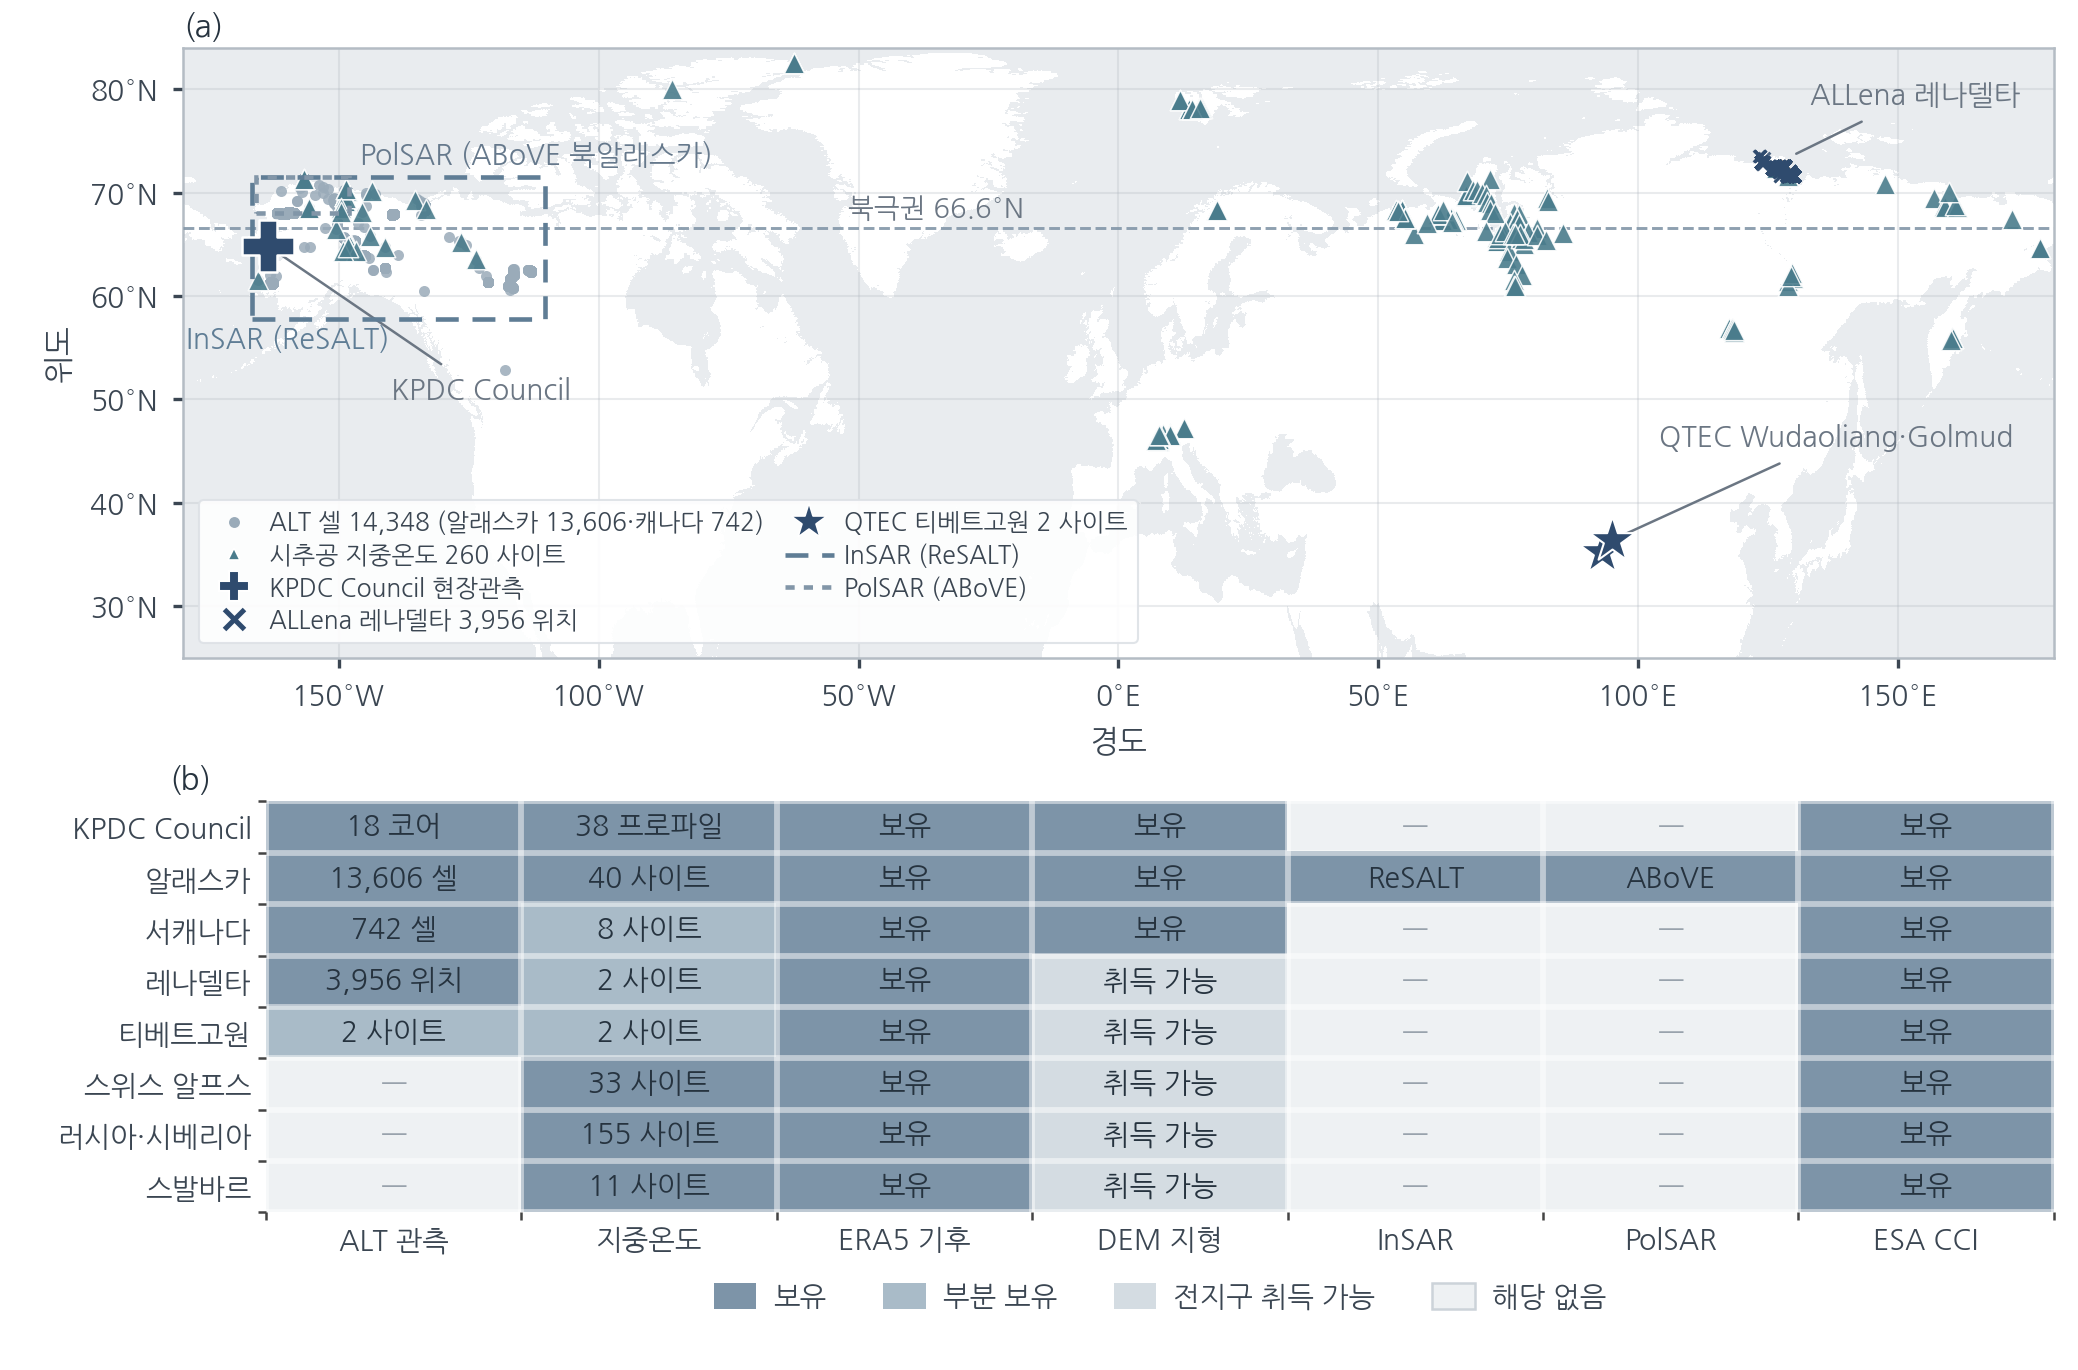
\includegraphics[width=0.78\textwidth]{../maps/data_inventory_world.png}
\caption{자료 인벤토리(학습·검증 이전의 원자료 분포). (a) ALT 관측·지중온도·물리관측·현장 자료의 지리 분포. (b) 지역별 자료 가용성. 관측 라벨은 알래스카·레나델타·캐나다의 소수 지점에 집중되며, 이 표본 편중이 라벨 희소의 구조적 원인이다.}
\label{fig:inventory}
\end{figure*}

\subsection{세 출처의 ALT 라벨}
ALT 값은 세 경로로 얻을 수 있으며, 각각을 후보 학습 신호로 두고 검증을 거쳐 사용 범위를 정하였다.
\begin{itemize}[leftmargin=1.1em,itemsep=1pt,topsep=2pt]
\item \textbf{실측 ALT.} 범북극 활동층 감시망(Circumpolar Active Layer Monitoring, CALM)과 북극-아한대 취약성 실험(Arctic-Boreal Vulnerability Experiment, ABoVE)의 알래스카 활동층 관측 13{,}606셀을 학습 기준으로 삼는다. 지역 간 전이 검증에는 러시아 시베리아 북동부 레나강 하구의 저지 삼각주인 레나델타(Lena Delta)의 융해 깊이 3{,}037셀과 캐나다 북서부 742셀을 사용한다. 세 지역은 기후·지형·토양이 서로 달라 전이 성능을 시험하기에 적합하다.
\item \textbf{지중온도 유도 ALT.} 지중온도 프로파일에서 여름 최대 융해면인 $0^\circ\mathrm{C}$ 등온선 깊이로 ALT를 유도한다. 국제 영구동토 관측망(Global Terrestrial Network for Permafrost, GTN-P)의 시추공 37지점과 KPDC 수어드반도 Council 사이트(이하 콘슬)의 19지점에서 확보하였다. 실측이 없는 곳에서도 관측에 근거한 값을 얻을 수 있어 증강 라벨의 유력한 후보이며, 실제 효과는 \S\ref{sec:derived}에서 검증한다. 본 연구에서는 표층 3차원 지중온도장의 학습 라벨과 예측 결과의 현장 검증에 사용한다.
\item \textbf{물리식 유도 ALT.} Stefan 식 등 물리경험식에 기후 공변량을 대입하여 ALT를 산출한다. 실측이 없는 지점에도 값을 제공하므로 증강 실험의 유사라벨은 이 경로로 생성하였다.
\end{itemize}

\begin{table}[H]
\centering
\footnotesize
\caption{ALT 라벨과 주요 자료원. 규모는 집계 후 셀 수이다. 위 세 자료원은 학습·평가에, 아래 두 자료원은 검증에 사용한다.}
\label{tab:data}
\begin{tabular}{@{}lp{2.3cm}r@{}}
\toprule
\tabhead{자료원} & \tabhead{대상·지역} & \tabhead{규모} \\
\midrule
CALM·ABoVE & 알래스카 활동층 & 13{,}606 \\
ALLena & 레나델타 융해 깊이 & 3{,}037 \\
ABoVE 캐나다 & 캐나다 활동층 & 742 \\
GTN-P & 시추공 지중온도 & 37 \\
KPDC Council & 수어드반도 지온·코어 & 19+18 \\
\bottomrule
\end{tabular}
\end{table}

\subsection{통합 스키마와 교차검증}
서로 다른 관측망을 하나의 표본 공간에 정렬하기 위해, 위치·공변량·라벨·자료원을 명시한 통합 스키마를 구축하였다. 스키마는 자료원마다 한 행을 두므로 전체 59{,}184행이며, 이 가운데 직접 관측이 17{,}386행이고 나머지는 CCI 제품(17{,}340), InSAR(14{,}348), PolSAR(10{,}073), 시추공(37)이다. 이를 고유 위치로 접으면 17{,}423셀이 된다.

공간 자기상관에 의한 성능 과대평가를 막기 위해 $0.5^\circ$ 공간블록을 집계 단위이자 교차검증 그룹으로 삼았고, 라벨에서 파생한 통계량은 입력에서 제외하였다. 평가는 두 축으로 한다. 같은 지역 내 일반화를 보는 공간블록 교차검증과, 한 지역에서 학습해 관측이 전혀 없는 다른 지역으로 넘어가는 지역 간 전이(leave-one-region-out)이다. 

\subsection{KPDC 현장 자료}
대회 자료인 KPDC의 콘슬 사이트에서 깊이 방향으로 7--16개 센서를 갖춘 일별 지중온도 프로파일 19지점(관측 연도별로 38개), 코어 융해 깊이 18개, 자동기상관측을 편입하였다. 콘슬은 최근접 학습 셀과 0.97\,km 떨어진 알래스카 지역 내 지점으로, 공변량 기반과 물성 이질성을 현장에서 검증하는 데 사용한다.


% =====================================================================
\section{방법}
% =====================================================================
표기에서 $\mathbf c(x)$는 위치 $x$의 공변량 벡터, $y$는 관측 ALT, $\mathcal T$는 학습 fold의 표본 집합이다.

\subsection{물리경험식}
물리경험식(이하 물리식)은 기후로부터 ALT를 직접 산출하여 증강의 공급원이자 예측기가 된다. 대표식인 Stefan 식[14]은 활동층 융해를 열전도 문제로 근사하여 융해 깊이를 누적 융해도일의 제곱근에 비례시킨다.
\begin{equation}
\mathrm{ALT}(x)=E\,\sqrt{\mathrm{TDD}(x)},\qquad
\mathrm{TDD}=\sum_{m}\max(\bar T_m,0)\,d_m
\label{eq:stefan}
\end{equation}
$\bar T_m$은 월평균 기온, $d_m$은 월 일수, $E$는 열·수분 물성을 묶은 계수이다. 계수 $E$는 각 학습 fold의 라벨에서만 추정하여($\hat E=\sum_{i\in\mathcal T}s_i y_i/\sum_{i\in\mathcal T}s_i^2$, $s_i=\sqrt{\mathrm{TDD}_i}$) 검증 누설을 막는다. Stefan 외에 edaphic, edaphic + TTOP 판정, Kudryavtsev, 열전도도 보정식을 함께 비교하여 어떤 물리식이 증강에 적합한지 판정한다.

\subsection{데이터 증강}
실측 라벨 집합을 $\mathcal D_{\mathrm{obs}}=\{(\mathbf c_i,y_i)\}_{i=1}^{n}$이라 하자. 여기에 실측이 없는 대상 지역의 위치 $x_k$에 물리식으로 산출한 유사라벨 $\tilde y_k$를 붙여 학습 집합을 확장한다.
\begin{equation}
\mathcal D_r=\mathcal D_{\mathrm{obs}}\cup\big\{(\mathbf c_k,\tilde y_k)\big\}_{k=1}^{n_{\mathrm{ps}}},
\ \ n_{\mathrm{ps}}=\lfloor r\,n\rfloor
\label{eq:aug}
\end{equation}
$r$은 증강 비율이다. 예를 들어 실측이 $n=13{,}606$개일 때 $r=1$이면 유사라벨을 같은 수만큼 더해 학습 집합이 두 배가 되고, $r=10$이면 유사라벨이 $136{,}060$개로 전체의 $91\%$를 차지한다. $r\in\{0,0.25,0.5,1,2,5,10\}$의 각 값에 대해 반복 평가한다. 유사라벨 $\tilde y$의 생성 규칙에 따라 세 조건을 둔다.
\begin{equation}
\tilde y_k=
\begin{cases}
\hat E\,\sqrt{\mathrm{TDD}(x_k)} & \text{(정확한 물리)}\\[2pt]
\mathrm{ALT}_{\mathrm{Ku}}(x_k) & \text{(부정확한 물리)}\\[2pt]
\bar y_{\mathrm{obs}} & \text{(대조, 상수)}
\end{cases}
\label{eq:pseudo}
\end{equation}
셋째 조건은 대조군이다. 물리 유사라벨과 동일한 대상 셀에 동일한 개수, 동일한 난수로 라벨을 붙이되 값만 학습 표본의 평균 ALT($\bar y_{\mathrm{obs}}=50.5\,\mathrm{cm}$) 상수로 대체한다. 두 조건은 학습에 노출되는 대상 지역 공변량과 유사라벨의 손실 가중이 완전히 같으므로, 성능 차이는 라벨이 담은 내용에서만 발생한다. 따라서 대조 대비 개선분은 대상 지역의 공변량 분포를 학습에 편입시킨 효과를 제거한 뒤 남는 물리 유사라벨 자체의 기여로 해석한다. 이를 유사라벨의 순가치로 정의한다.
\begin{equation}
\begin{aligned}
\Delta_{\mathrm{phys}}(r)=\;&\big[\mathrm{RMSE}_{0}-\mathrm{RMSE}^{\mathrm{phys}}_{r}\big]\\
-\;&\big[\mathrm{RMSE}_{0}-\mathrm{RMSE}^{\mathrm{ctrl}}_{r}\big]
\end{aligned}
\label{eq:netvalue}
\end{equation}
$\Delta_{\mathrm{phys}}>0$이면 개선이 물리 정보에서 온 것이다. 예를 들어 증강 전 오차가 $34.0$이고 물리 유사라벨로 $31.8$, 상수 라벨로 $42.0\,\mathrm{cm}$가 되었다면 물리는 $2.2$를 줄이고 상수는 $8.0$을 늘렸으므로 순가치는 $2.2-(-8.0)=10.2\,\mathrm{cm}$이다. 다만 상수 라벨은 유사라벨의 수준과 공간 변동을 동시에 제거하므로, 이 값은 물리식이 제공하는 수준 보정과 공간 구조 기여를 합한 양이다. 유사라벨을 붙이는 셀과 평가 셀은 $0.5^\circ$ 공간블록 단위로 분리하여 서로 인접하지 않게 하였다.

\subsection{기계학습·딥러닝 모델군}
증강된 학습 집합 $\mathcal D_r$로 ALT를 회귀하는 모델 $f_\theta$를 동일 조건에서 비교한다.
\begin{equation}
\hat\theta=\arg\min_{\theta}\sum_{(\mathbf c,y)\in\mathcal D_r}\big(y-f_\theta(\mathbf c)\big)^2 .
\label{eq:fit}
\end{equation}
모델군은 트리 부스팅(HistGBM, LightGBM, XGBoost, CatBoost[19])과 신경망(다층 퍼셉트론, FT-Transformer[20], TabM[21])이며, 신경망 입력은 학습 fold 내부 통계로 표준화한다.

물리와 데이터를 결합하는 구조로, 물리식 예측을 기준선으로 두고 그 위에 잔차 모델 $g$를 더한다.
\begin{equation}
\hat y(x)=\underbrace{\hat E\sqrt{\mathrm{TDD}(x)}}_{\text{물리 기준선}}
+\;\lambda\, g\big(\mathbf c(x)\big),\ \ \lambda\in[0,1]
\label{eq:residual}
\end{equation}
$g$는 물리식이 설명하지 못한 나머지, 곧 잔차 $y_i-\hat E s_i$를 학습한다. 물리식이 어떤 지점에서 $45\,\mathrm{cm}$를 예측했는데 실측이 $52\,\mathrm{cm}$라면 잔차는 $+7\,\mathrm{cm}$이고, 모델은 공변량으로부터 이 $+7$을 맞추도록 학습한다. 과적합을 막기 위해 능형 회귀와 얕은 부스팅 같은 저용량 모델을 사용한다. $\lambda$는 잔차의 반영 정도를 조절하는 가중으로, $\lambda=0$이면 순수 물리식, $\lambda=1$이면 잔차를 온전히 반영한다.

\subsection{표층 3차원 지중온도장과 시계열}
표층 3차원 지중온도장은 공변량과 깊이 변수를 함께 입력하여 각 깊이의 연최대 지온을 회귀하는 모델로 구성하고, 깊이에 대한 단조성을 제약하여 물리적으로 타당한 프로파일을 얻는다. 융해면은 예측된 온도 프로파일이 $0^\circ\mathrm{C}$를 지나는 깊이를 선형보간하여 구한다. 연별 ALT 지도는 식~\eqref{eq:stefan}에 그해의 기후 입력을 대입하여 생성한다.

\subsection{평가와 보정 불확실성}
정확도는 평균제곱근오차로 측정한다.
\begin{equation}
\mathrm{RMSE}=\sqrt{\tfrac1m\sum_{j=1}^{m}\big(y_j-\hat y_j\big)^2}.
\label{eq:rmse}
\end{equation}
지역 간 전이는 표본이 알래스카에 편중된 영향을 배제하기 위해, 지역 집합 $\mathcal R$에 대한 지역별 오차의 비가중 평균을 기준으로 한다.
\begin{equation}
\mathrm{RMSE}_{\mathrm{transfer}}=\frac{1}{|\mathcal R|}\sum_{\rho\in\mathcal R}\mathrm{RMSE}_{\rho}.
\label{eq:transfer}
\end{equation}
예측구간은 분위 회귀로 상·하한 $\hat q_{lo},\hat q_{hi}$를 얻은 뒤 등순응 분위 회귀(Conformalized Quantile Regression, CQR[18])로 보정한다. 학습 블록 내부에서 분리한 보정 표본 $\mathcal C$에서 순응 점수를 계산하고, 그 분위 $Q_c$만큼 구간을 넓힌다.
\begin{equation}
\begin{aligned}
E_i&=\max\big(\hat q_{lo}(x_i)-y_i,\;y_i-\hat q_{hi}(x_i)\big),\ i\in\mathcal C,\\
\hat C_c(x)&=\big[\hat q_{lo}(x)-Q_c,\;\hat q_{hi}(x)+Q_c\big].
\end{aligned}
\label{eq:cqr}
\end{equation}
아울러 적용가능 영역(Area of Applicability, AOA[17])을 비유사도지수(Dissimilarity Index, DI)로 정의한다. 표준화한 공변량 공간에서 예측점과 가장 가까운 학습점 사이의 거리를, 학습 표본 내부의 평균 최근접 거리 $\bar d$로 정규화한 값이다.
\begin{equation}
\mathrm{DI}_k=\frac{\min_{i\in\mathcal T}\lVert \tilde{\mathbf c}_k-\tilde{\mathbf c}_i\rVert_2}{\bar d}
\label{eq:di}
\end{equation}
DI가 학습 분포의 상위 임계를 넘는 지점은 외삽 영역으로 표기하여, 지도에서 신뢰 범위를 벗어난 곳을 구분한다.


\begin{figure*}[!t]
\centering
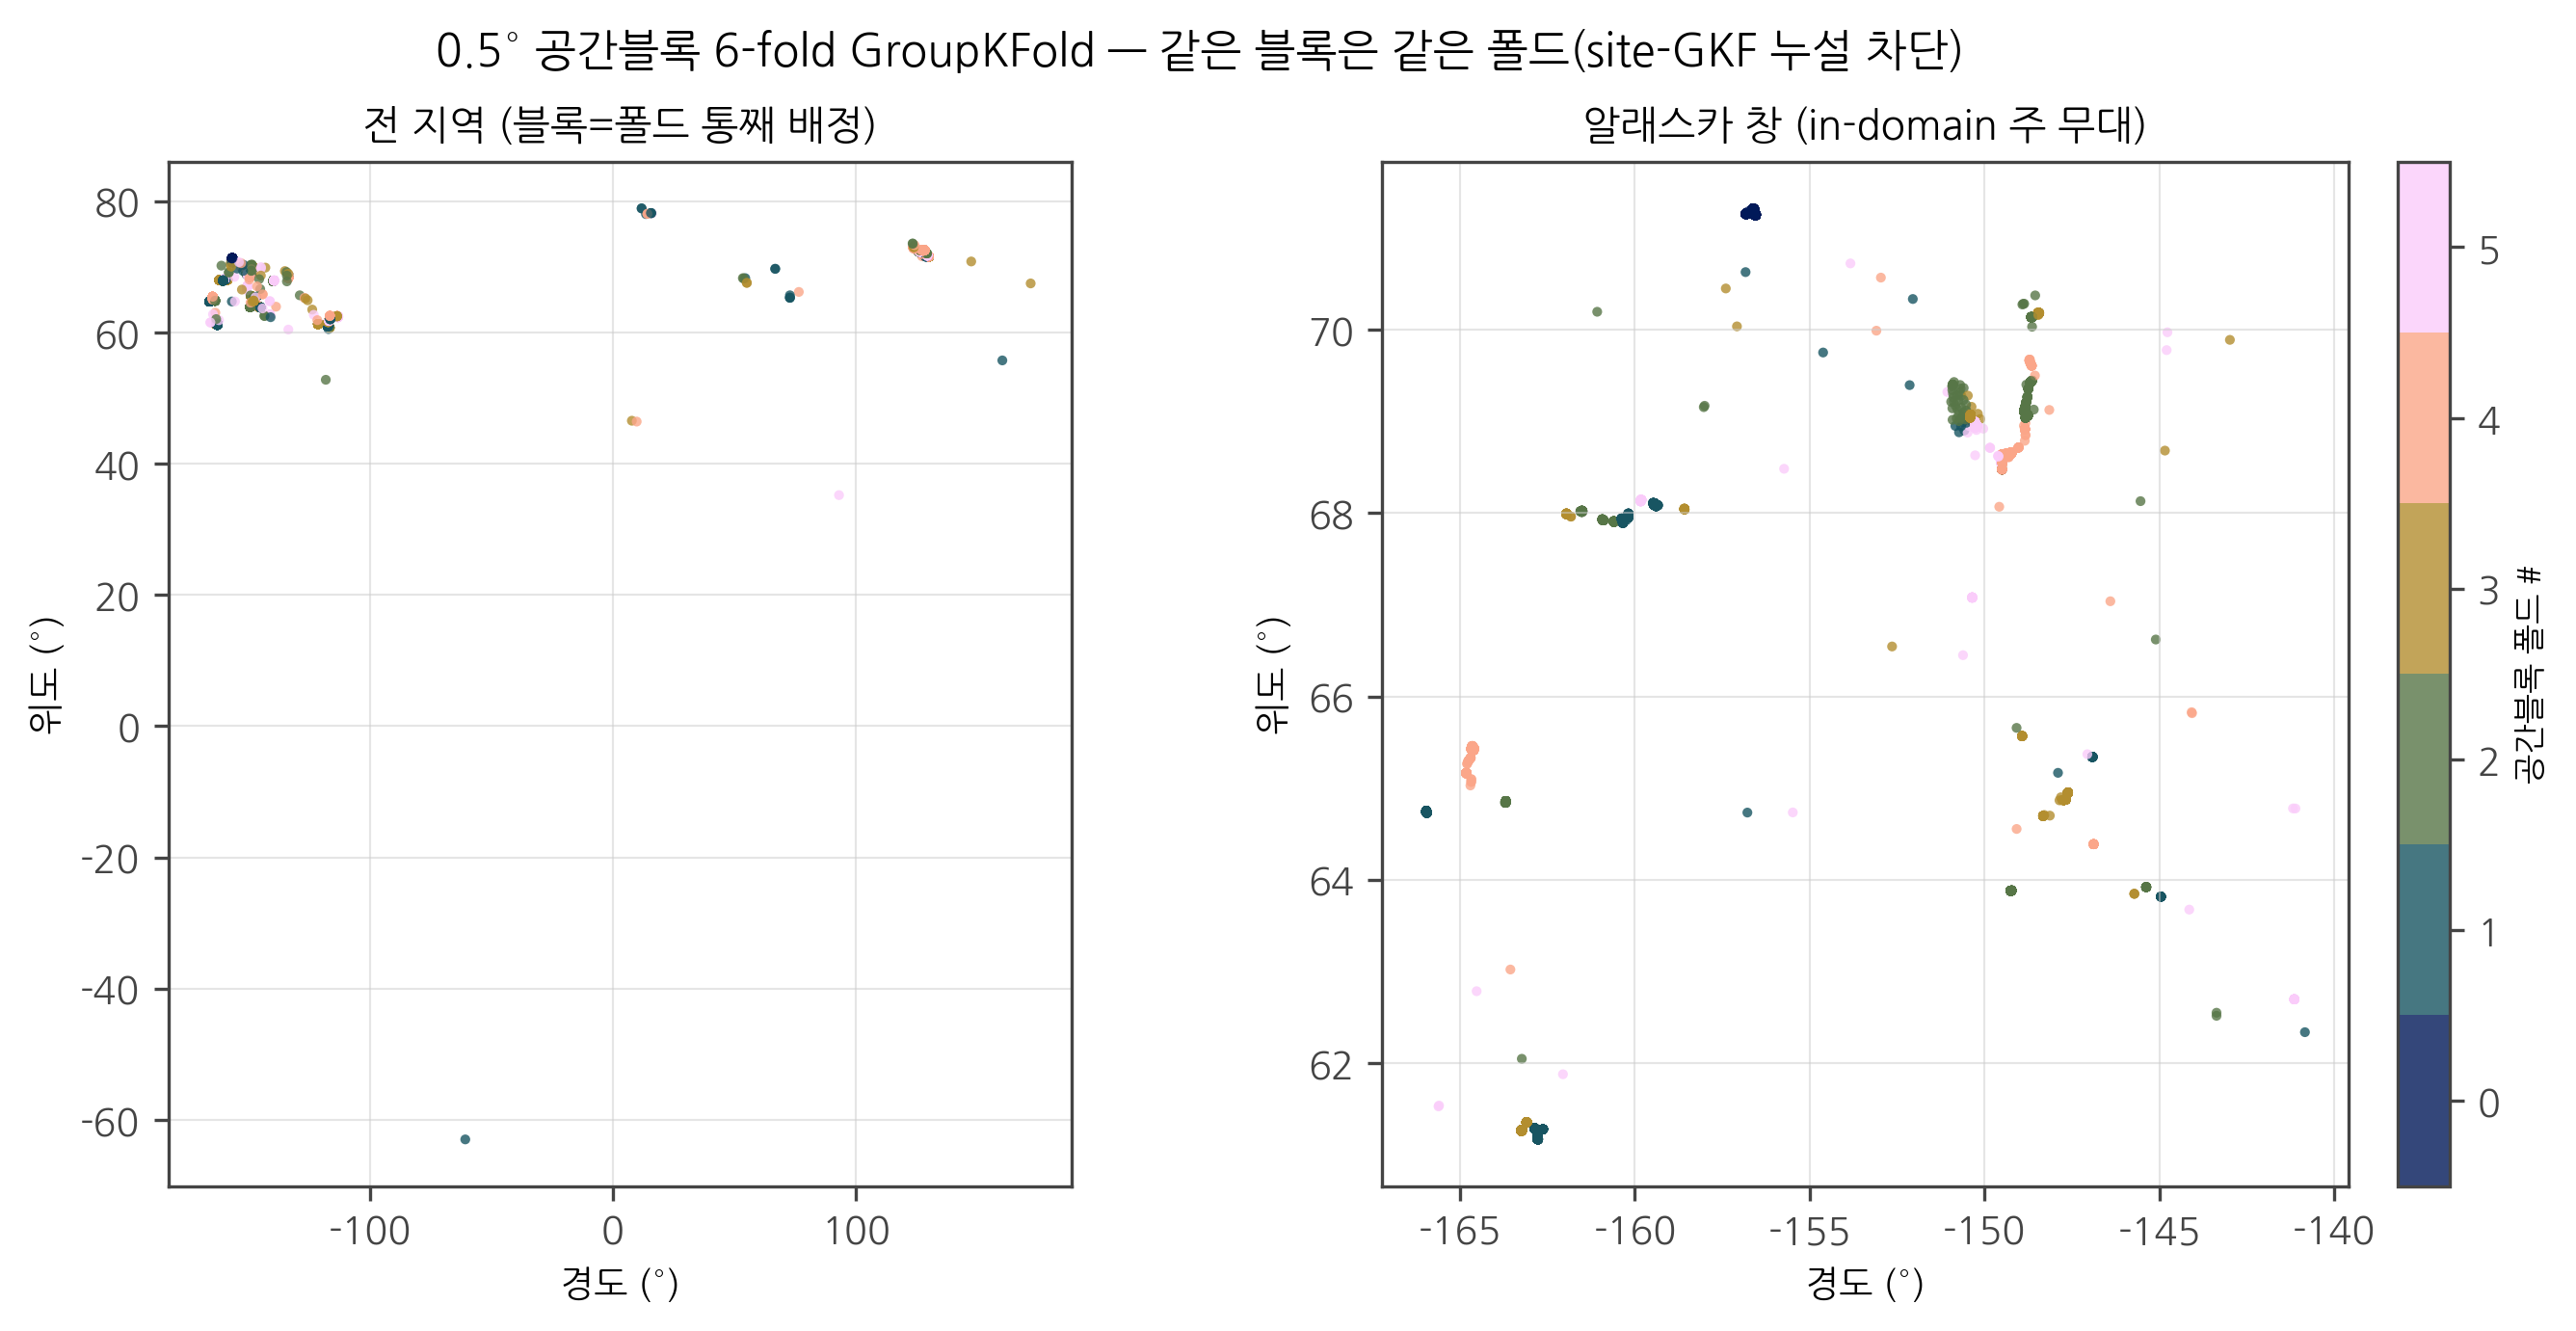
\includegraphics[width=0.9\textwidth]{../figures/s0_schema/spatial_block_folds_map.png}
\caption{공간블록 교차검증의 fold 배정. $0.5^\circ$ 격자 블록을 그룹으로 하여 같은 블록의 관측은 반드시 같은 fold에 배정된다. 색은 fold 번호이다. (a) 범북극 관측 분포와 알래스카 범위(파선은 $66.5^\circ$N), (b) 알래스카의 블록별 fold 배정, (c) 북부 알래스카 확대로 본 블록 격자와 그 안의 관측. 하나의 fold는 서로 인접하지 않은 여러 블록을 포함할 수 있으므로 (c)에서 같은 fold 번호가 떨어진 칸에 반복해 나타난다. 이 설계가 공간 자기상관에 의한 낙관 편향을 차단한다.}
\label{fig:folds}
\end{figure*}


% =====================================================================
\section{결과}
% =====================================================================
결과는 대상 지역의 정보를 학습에 얼마나 쓸 수 있는가에 따라 세 조건으로 나뉜다(표~\ref{tab:settings}). 조건이 다르면 학습 집합과 평가 셀이 모두 달라지므로, 서로 다른 조건의 수치를 같은 축에 놓고 비교하지 않는다. 이하 각 절과 그림은 어느 조건에 해당하는지를 함께 밝힌다.

\begin{table}[H]
\centering
\footnotesize
\caption{결과 절의 검증 조건. 세 조건은 대상 지역 정보의 가용 범위로만 구분된다. 평가 지역이 달라 조건 간 수치를 직접 비교할 수 없다.}
\label{tab:settings}
\begin{tabular}{@{}p{0.20\columnwidth}p{0.30\columnwidth}p{0.38\columnwidth}@{}}
\toprule
\tabhead{조건} & \tabhead{대상 지역 정보} & \tabhead{평가} \\
\midrule
지역 내 & 실측 라벨까지 사용 & 알래스카 $0.5^\circ$ 공간블록 교차검증 \\[2pt]
공변량만 & 공변량은 사용, 실측 라벨 없음 & 대상 지역을 공간블록으로 이분하여 한쪽으로 학습, 다른 쪽 실측으로 평가 \\[2pt]
정보 없음 & 학습에 일절 사용 불가 & 지역 단위 홀드아웃 \\
\bottomrule
\end{tabular}
\end{table}

\subsection{데이터 재구조화와 모델 비교}
\emph{조건: 지역 내.}
관측은 소수 지점에 밀집해 있어, 지점 단위로 평가하면 밀집 지역이 결과를 지배한다. 이를 보정하기 위해 $0.5^\circ$ 셀 단위로 집계하고 위치마다 동등 가중을 부여하였다. 지점 단위로 채점할 때와 견주면 이 재구조화만으로 추가 자료 없이 같은 지역 내 예측이 약 $11\%$, 지역 간 전이가 약 $7\text{--}8\%$ 개선된다. 이후 모든 실험은 이 기준선 위에서 수행하였다.

같은 기준선에서 실측 라벨만으로 학습한 기계학습·딥러닝 7종을 비교하였다(표~\ref{tab:models}, 그림~\ref{fig:models}). 알래스카 지역 내 검증에서 신경망(다층 퍼셉트론·TabM)이 약 $14.4\,\mathrm{cm}$로 가장 낮고, 물리식 단독(Stefan)이 $14.56\,\mathrm{cm}$로 이에 근접하며, 부스팅이 $15.6\text{--}17.2\,\mathrm{cm}$로 뒤를 잇는다.

상위권의 간격은 좁다. 알래스카 관측 ALT의 표준편차가 $17.4\,\mathrm{cm}$이므로 전체 평균만 예측해도 $17.4\,\mathrm{cm}$가 나온다. 즉 상위 모델의 $14.4\,\mathrm{cm}$는 평균 예측 대비 약 $17\%$ 개선에 해당하며, 신경망과 물리식의 차이는 난수 seed 변동 범위 안이다. 이는 모델 구조를 바꾸는 것만으로는 정확도를 크게 끌어올리기 어렵다는 뜻이며, 학습 신호 자체를 늘리는 증강이 필요한 이유이기도 하다. 한편 기후 자료는 광역에서 조밀하게 확보되므로, 물리경험식을 세분 격자에 적용하면 관측이 없는 곳까지 연속적인 ALT 장을 산출할 수 있다(그림~\ref{fig:hires}).

이때 지도의 실효 해상도는 격자 간격이 아니라 입력 자료가 담은 정보의 규모로 정해진다. 기후 자료는 $11\,\mathrm{km}$, 토양 자료는 $5\,\mathrm{km}$ 간격이므로 이들만 사용하면 격자를 아무리 잘게 나누어도 그보다 세밀한 구조는 생기지 않는다. 반면 수치표고모형은 $30\,\mathrm{m}$ 간격으로 확보되므로, 지형 공변량을 함께 넣으면 훨씬 작은 규모의 구조를 재현할 수 있다. 실제로 브룩스 산맥 북사면에서 북극 연안평야에 이르는 영역을 두 조건으로 산출하면, 지형을 포함한 $243\,\mathrm{m}$ 격자 산출물에서 하천망과 사면을 따르는 융해 깊이의 변화가 드러난다(그림~\ref{fig:downscale}). 세부 구조의 크기를 국소 고주파 성분의 표준편차로 재면 기후·토양만 사용한 경우 $0.47\,\mathrm{cm}$인 데 비해 지형을 포함하면 $2.91\,\mathrm{cm}$로 여섯 배가 된다. 다만 앞의 변수그룹 제거 실험에서 보았듯 지형은 셀 평균 규모의 정확도를 크게 높이지는 못하므로, 이 세부 구조는 검증된 정확도 향상이 아니라 지형이 시사하는 공간 변동으로 해석해야 한다.

\begin{table}[H]
\centering
\footnotesize
\caption{실측 라벨로 적합한 모델의 지역 내 ALT 예측(참조로 물리식과 평균 예측을 함께 제시). 알래스카 공간블록 교차검증, 입력 34종, 3-seed 앙상블 예측 기준. Stefan은 공변량 학습 없이 계수 $E$ 하나만 학습 fold에서 적합하므로 확률 성분이 없다.}
\label{tab:models}
\begin{tabular}{@{}lrl@{}}
\toprule
\tabhead{모델} & \tabhead{RMSE(cm)} & \tabhead{비고} \\
\midrule
다층 퍼셉트론 & 14.37 & 신경망 최상 \\
TabM & 14.40 & 다층 퍼셉트론과 동률 \\
Stefan 물리식 & 14.56 & 계수 1개만 적합 \\
CatBoost & 15.61 & 부스팅 최상 \\
XGBoost & 16.16 & \\
LightGBM & 16.48 & \\
HistGBM & 17.21 & 부스팅 하위 \\
(평균 예측) & 17.38 & 참조 기준선 \\
FT-Transformer & 18.56 & 지역 내 최하 \\
\bottomrule
\end{tabular}
\end{table}


\begin{figure*}[!t]
\centering
\begin{subfigure}[t]{0.5\textwidth}
  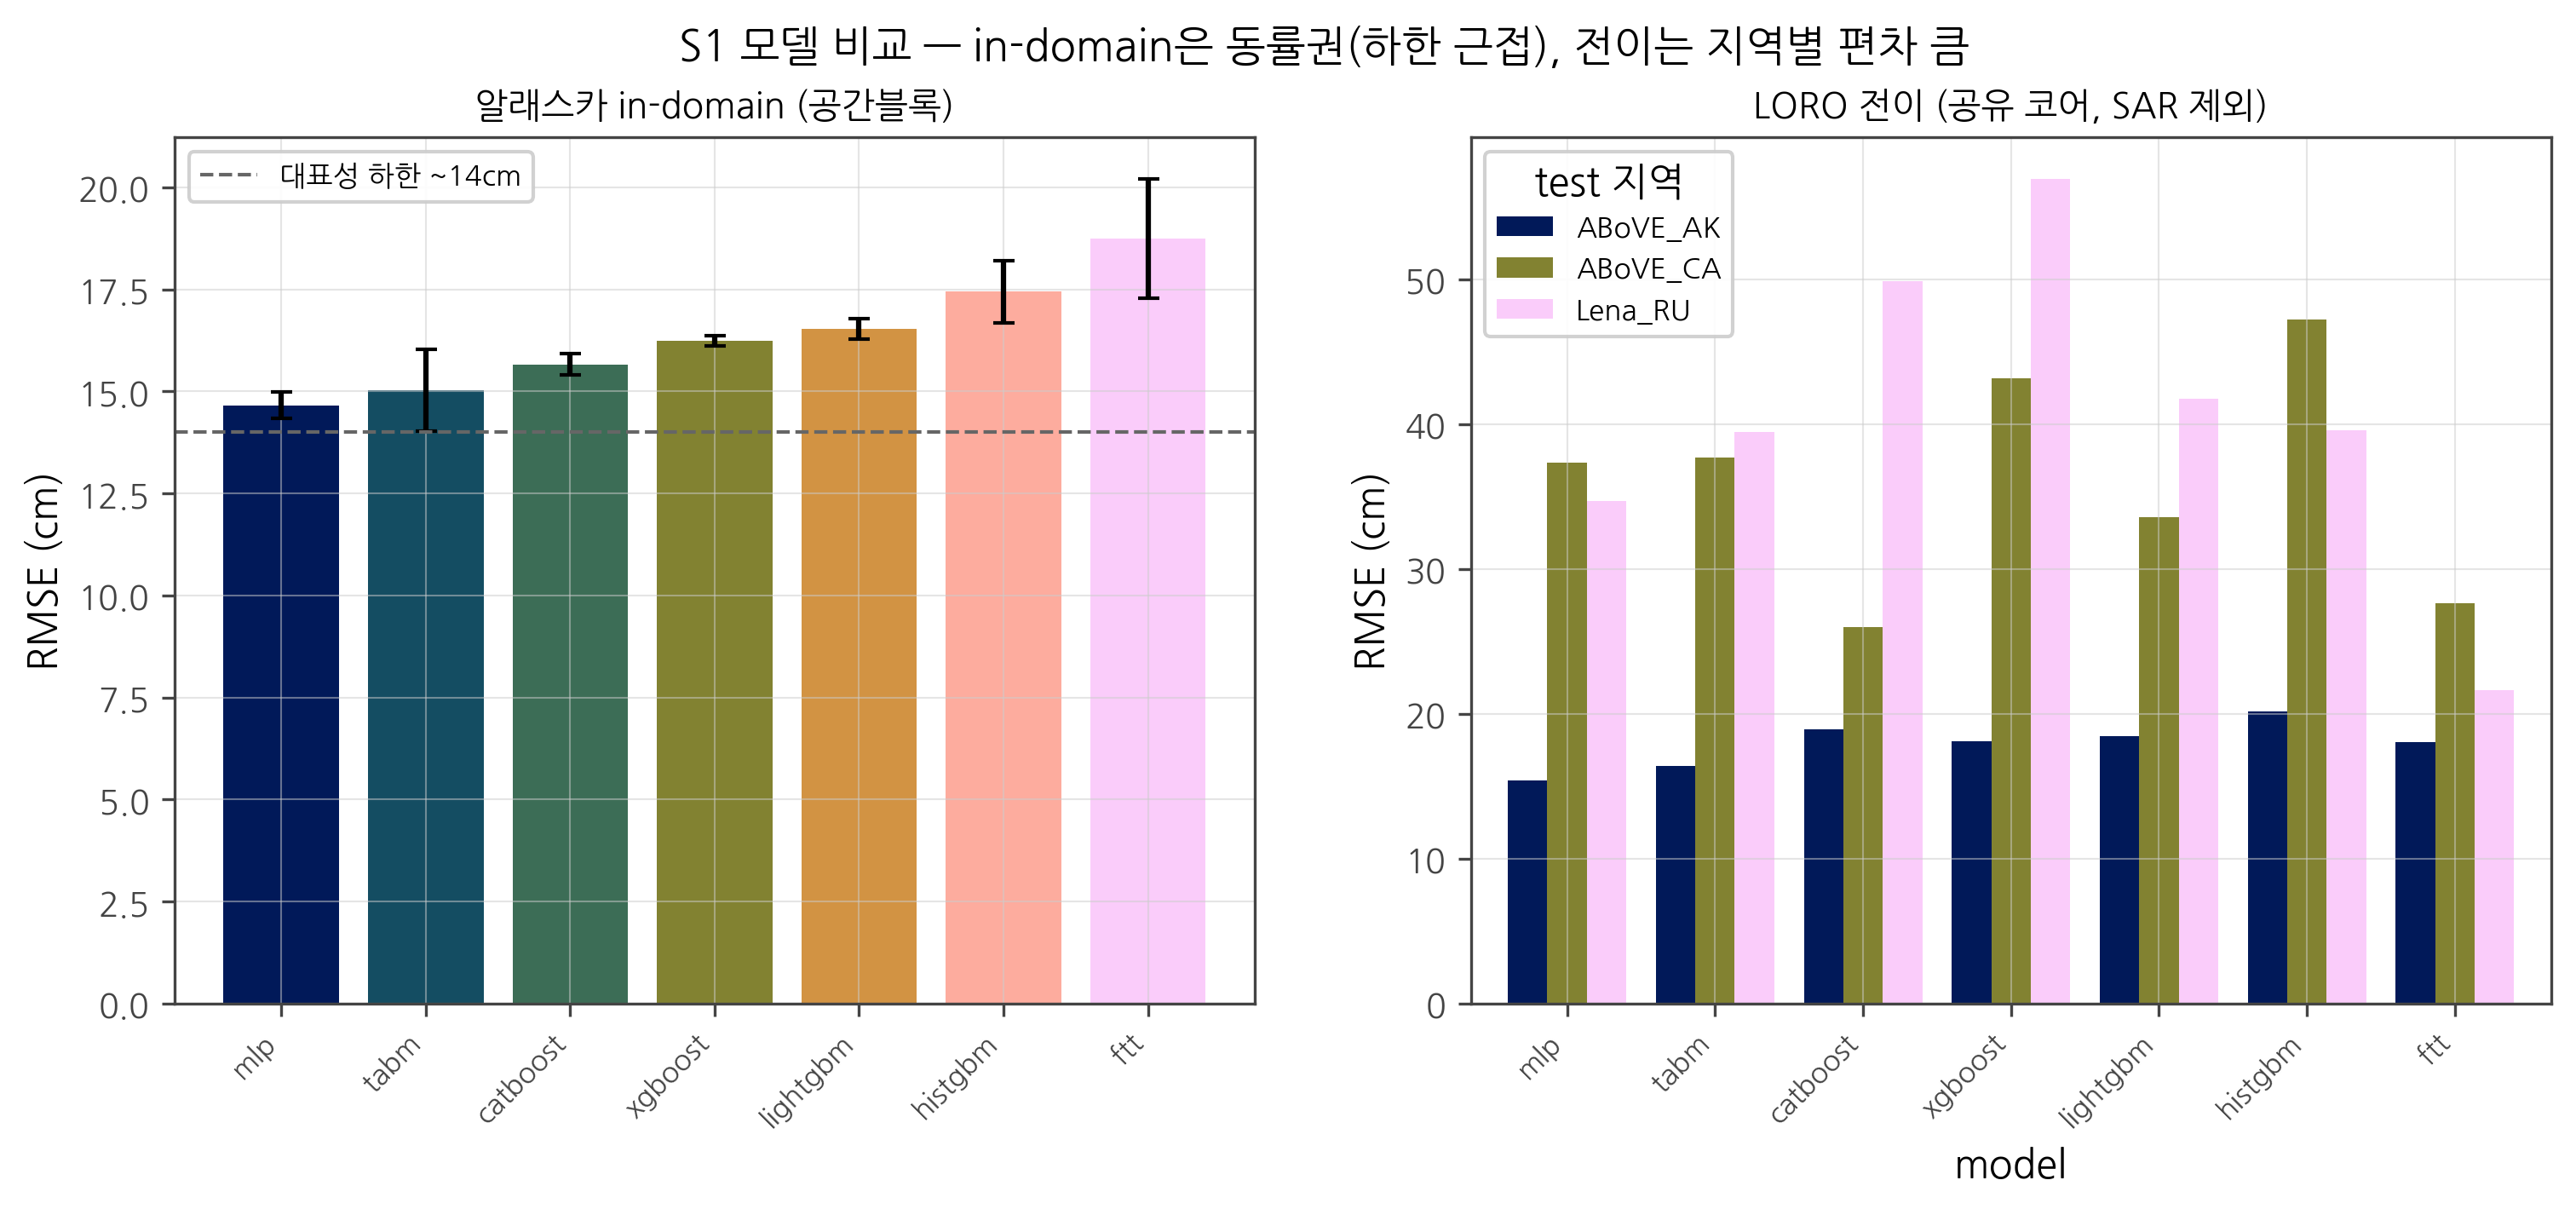
\includegraphics[width=\linewidth]{../figures/s1_baseline/model_comparison_bars.png}
  \caption{기계학습·딥러닝 7종의 예측 오차. 실측 라벨 학습, 입력 34종, 알래스카 공간블록 교차검증, 3-seed 앙상블 예측 기준으로 표~\ref{tab:models}과 같은 값이다. 세로선은 표의 참조 두 행(물리식 단독·평균 예측)이다. 상위권의 간격이 좁고, 전 모델이 지점 관측 대표성 하한 위에 놓인다.}
  \label{fig:modelbars}
\end{subfigure}\hfill
\begin{subfigure}[t]{0.47\textwidth}
  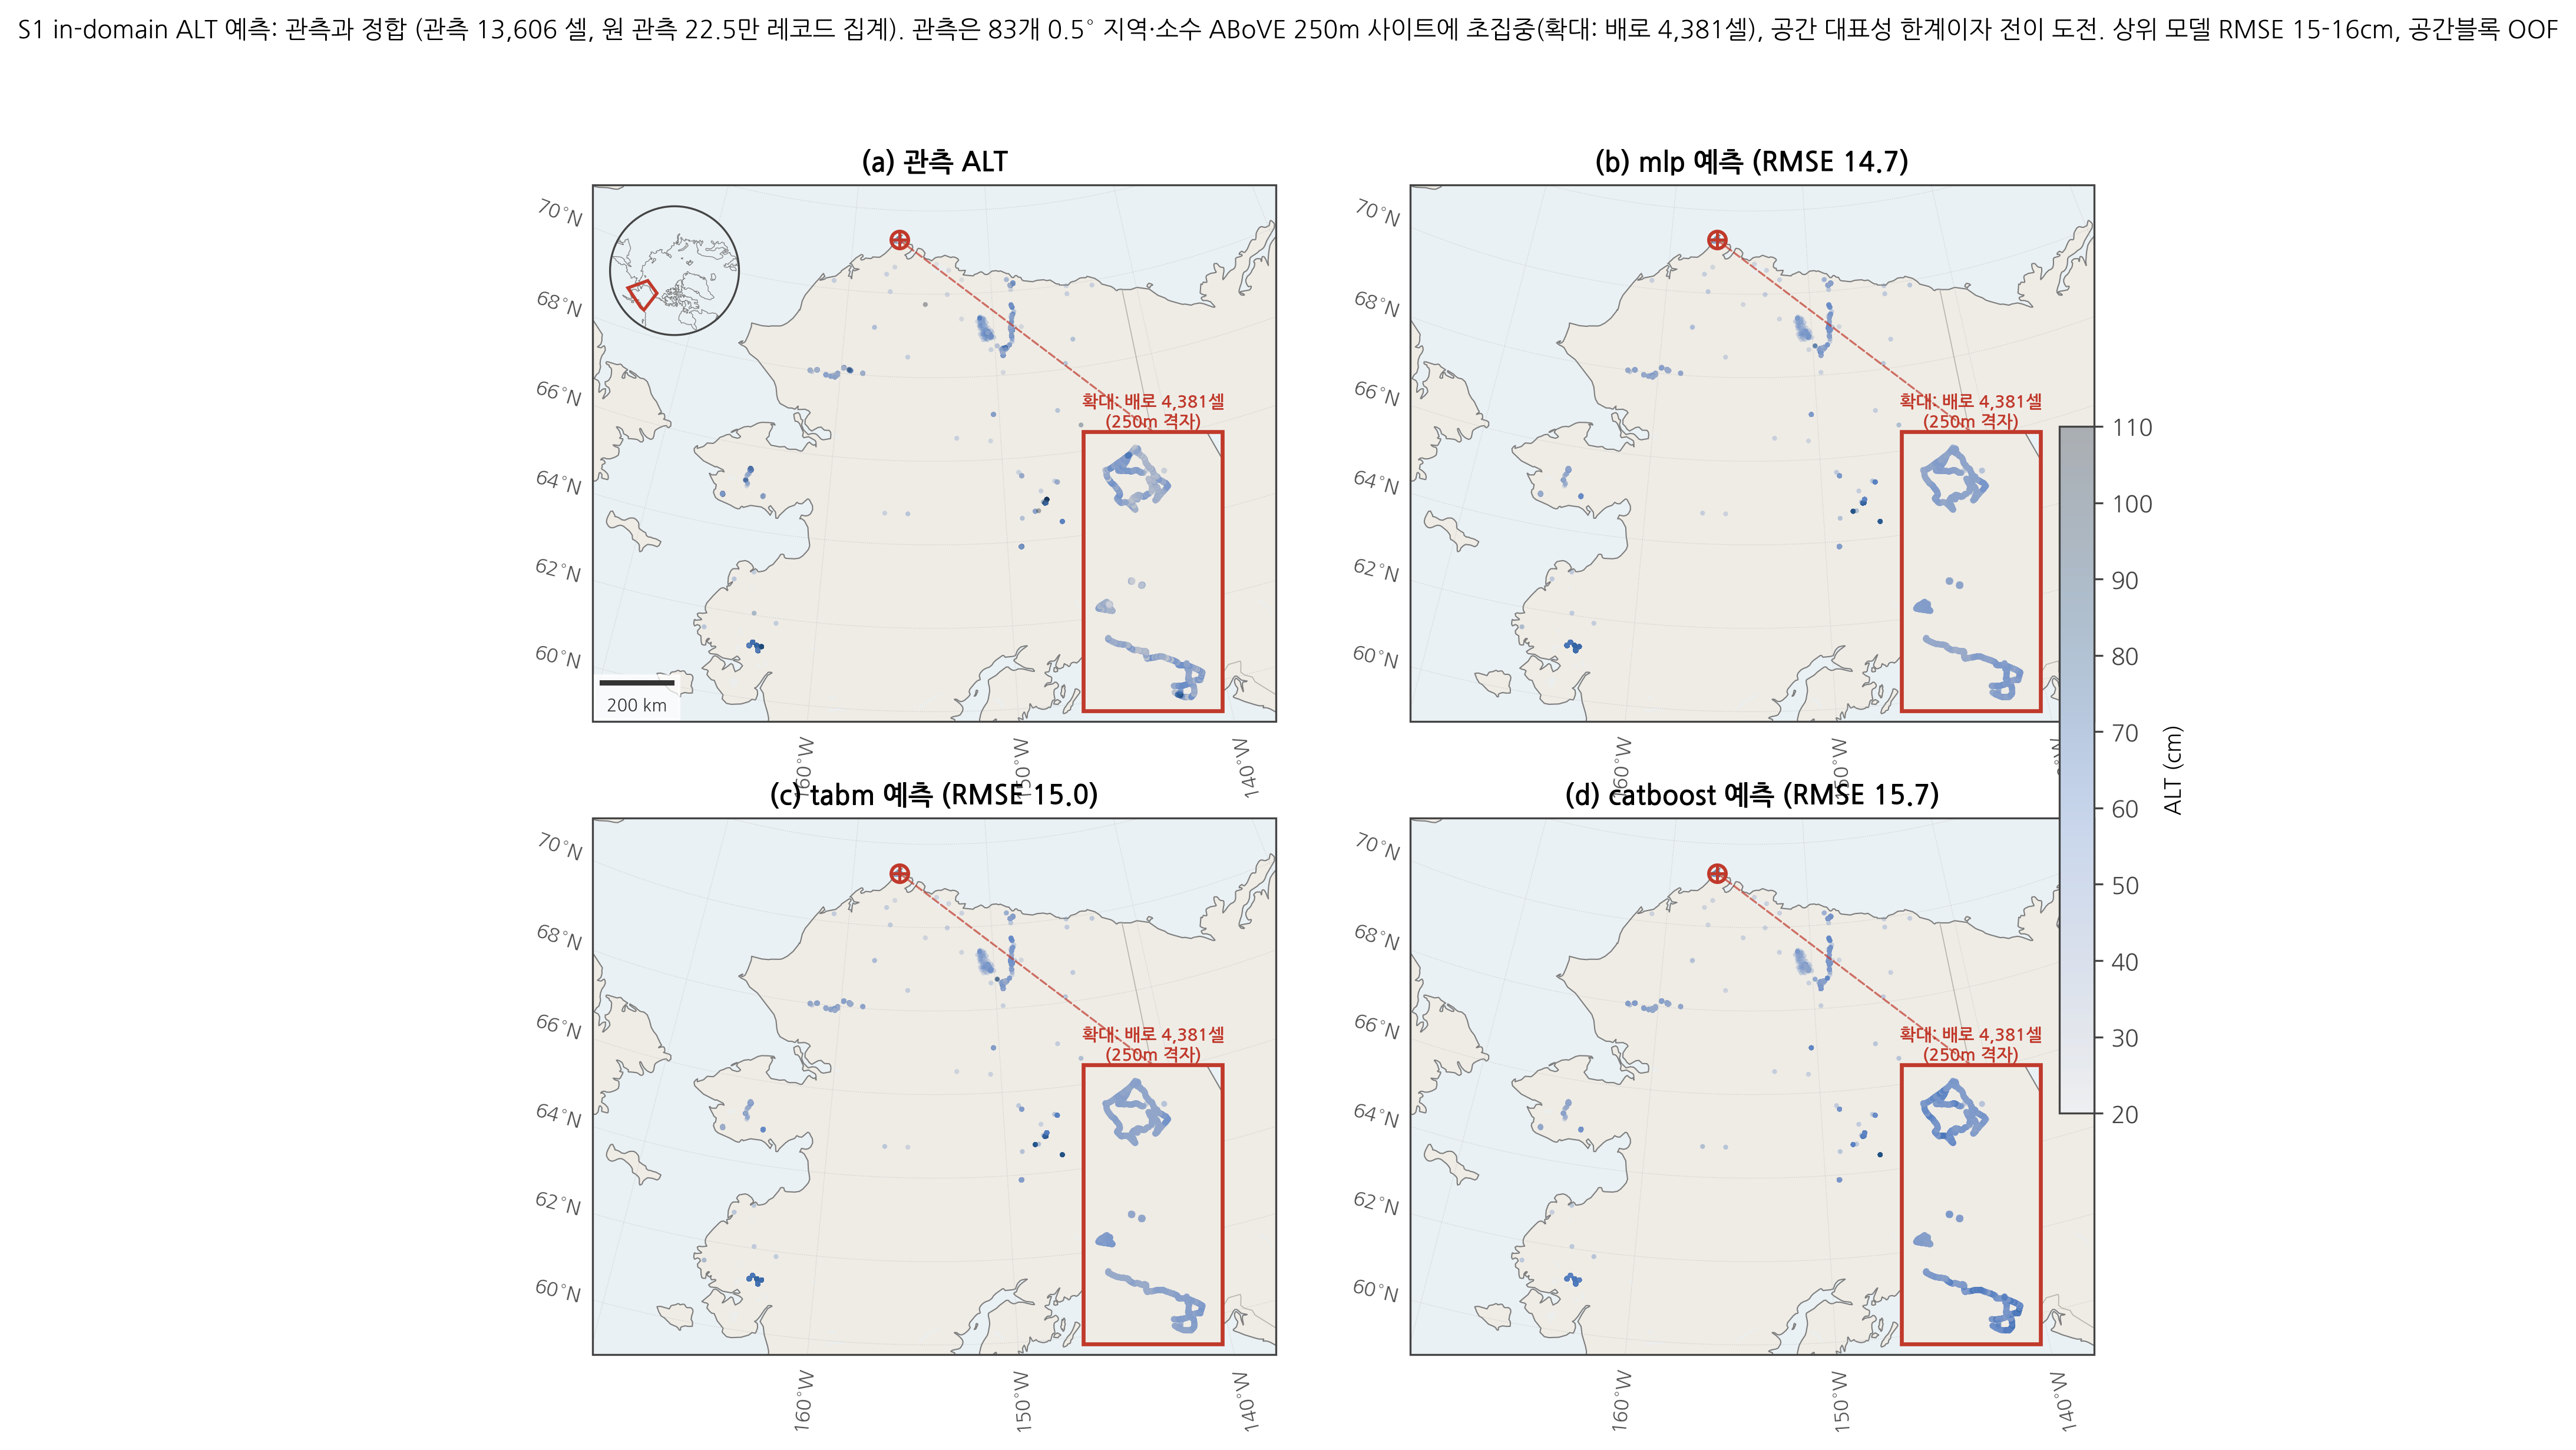
\includegraphics[width=\linewidth]{../figures/s1_baseline/alaska_obs_vs_pred_maps.png}
  \caption{관측 ALT와 상위 3모델(MLP·TabM·CatBoost)의 교차검증 예측을 같은 색 범위로 나란히 그린 지도. 우하단은 최대 밀집지(배로) 확대이다. 예측장은 광역이나 관측 라벨은 소수 지점에 집중된다.}
  \label{fig:s1maps}
\end{subfigure}
\caption{기계학습·딥러닝 모델 비교와 알래스카 예측 지도(모두 알래스카 지역 내 검증).}
\label{fig:models}
\end{figure*}

\begin{figure*}[!t]
\centering
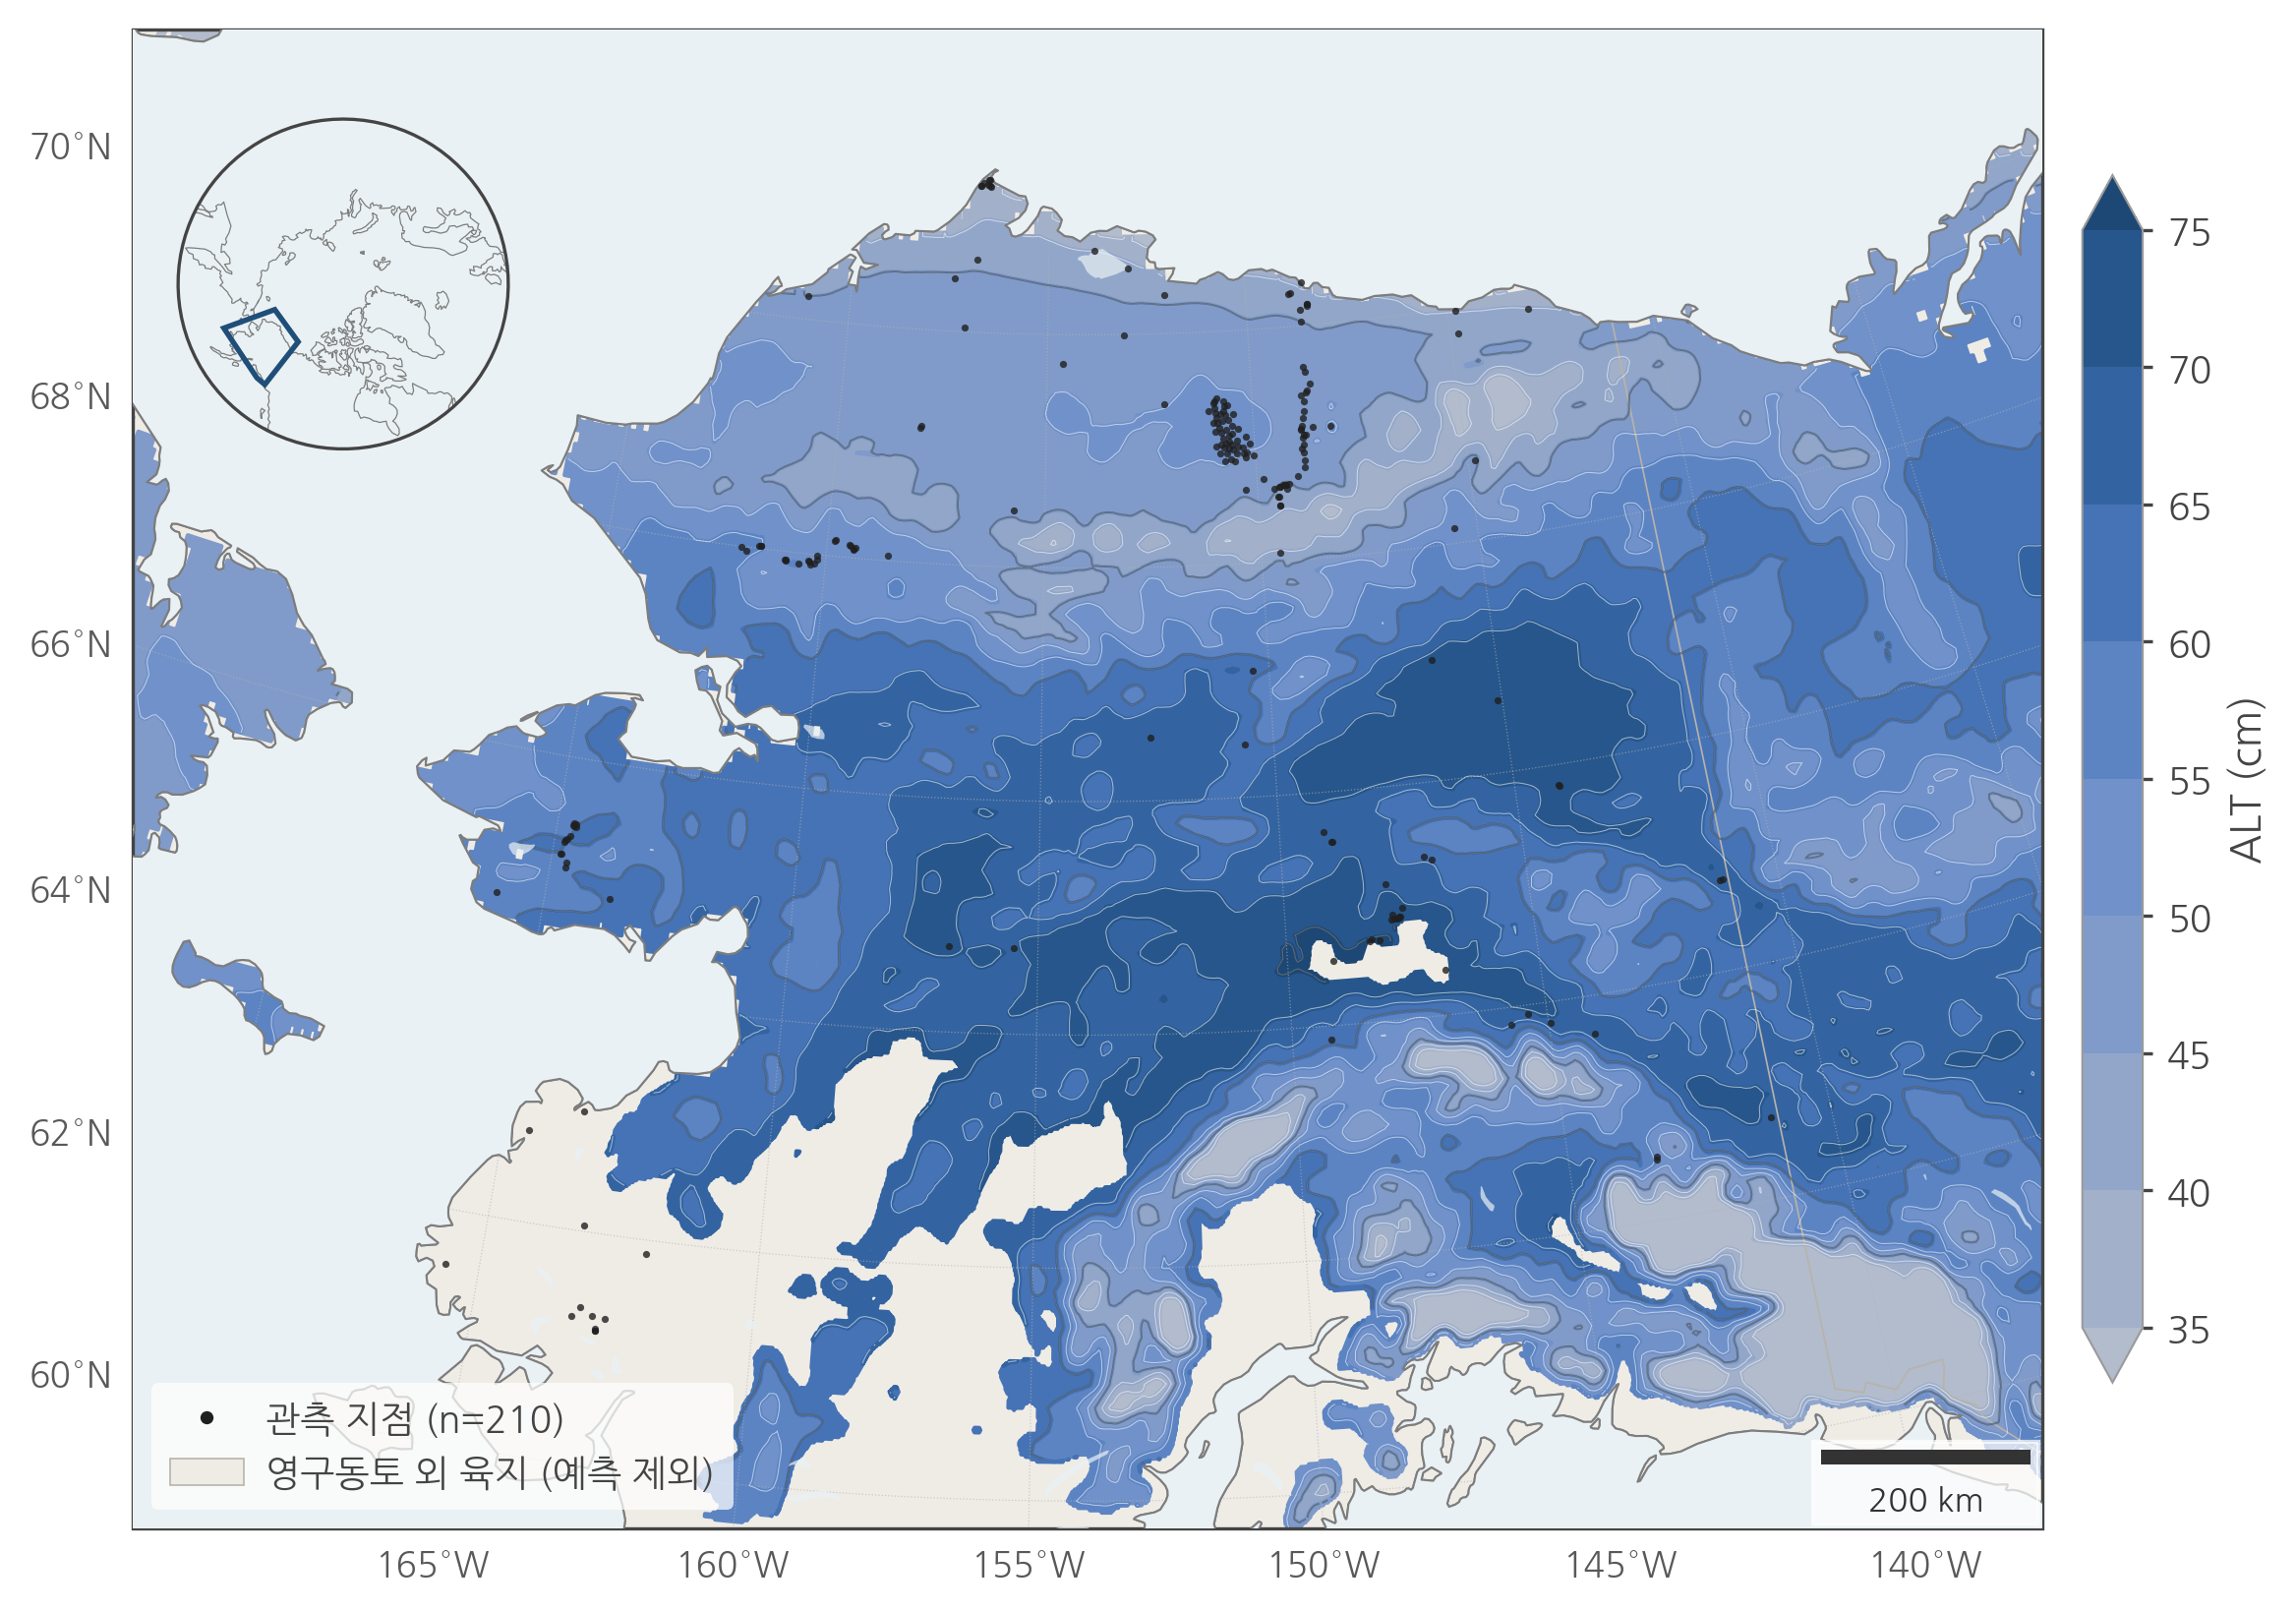
\includegraphics[width=0.82\textwidth]{../maps/alt_prediction_hires.png}
\caption{알래스카 영구동토 지대의 고해상 ALT 예측장. 모델은 물리식 단독(Stefan, 식~\eqref{eq:stefan})이며 계수 $E$는 알래스카 실측에 최소제곱으로 적합하였다. ERA5-Land 월 기후값(2015--2020)을 $0.02^\circ$ 격자로 세분하고 토양 물성은 SoilGrids $5\,\mathrm{km}$ 자료를 사용하였다. 영구동토 범위는 다년평균 연평균기온 $<0^\circ\mathrm{C}$로 정의하였고(육지의 $84.8\%$), 그 밖의 육지는 예측을 표시하지 않았다. 검은 점은 관측 지점이다. 잔차 학습을 얹은 결합 모델이 지역 내에서 더 정확하지만, 그 모델은 학습 공변량 분포 안에서만 유효하므로(그림~\ref{fig:uqmap}) 광역 연속장에는 전 격자에서 산출 가능한 물리식 단독을 쓴다. 이 지도와 그림~\ref{fig:s9}는 같은 계수와 같은 영구동토 판정 기준을 쓰되, 기후값 기간이 각각 2015--2020년과 2010--2024년으로 달라 마스크 경계가 완전히 일치하지는 않는다.}
\label{fig:hires}
\end{figure*}

\begin{figure*}[!t]
\centering
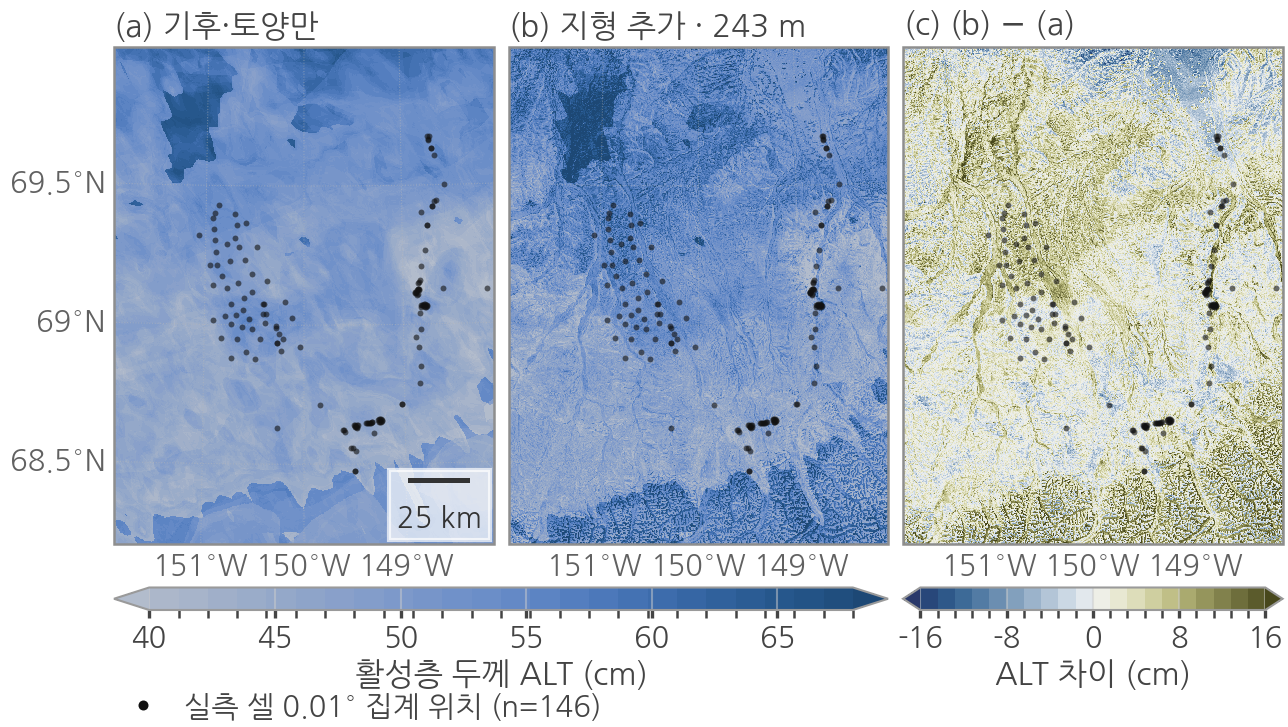
\includegraphics[width=0.90\textwidth]{../maps/alt_downscale_demo.png}
\caption{지도의 실효 해상도를 결정하는 요인. 알래스카 북사면($-152$에서 $-148^\circ$E, $68.2$에서 $70.0^\circ$N)의 같은 영역을 (a) 기후($11\,\mathrm{km}$)와 토양($5\,\mathrm{km}$) 공변량만으로, (b) $30\,\mathrm{m}$ 수치표고모형에서 유도한 지형 공변량을 더해 $243\,\mathrm{m}$ 격자로 산출한 결과이다. (c)는 두 결과의 차이이며, 하천망과 사면을 따르는 공간 구조가 지형에서 온다. (a)는 지형 변수를 영역 중앙값으로 고정한 대조이므로 (c)에는 그 고정에서 오는 수준 차이가 함께 들어 있다. 읽어야 할 것은 차이의 절대 크기가 아니라 공간 패턴이다. 격자를 잘게 나누는 것만으로는 세부가 생기지 않으며 세밀한 입력 자료가 있어야 한다.}
\label{fig:downscale}
\end{figure*}


\subsection{물리경험식의 선택}
\emph{조건: 학습 없음(산출식만). 지역 내와 정보 없음 두 축에서 각각 평가.}
물리식은 표현하려는 과정에 따라 분화되었다. Stefan 식은 융해 전선의 잠열 수지만으로 문제를 기술하고 토양 물성을 계수 $E$ 하나로 집약한다. Kudryavtsev 식[15]은 Stefan이 무시한 적설 절연과 식생 차폐, 토양 수분의 열전도 효과를 연중 온도 진폭의 감쇠 단계로 명시한다. 나머지 세 변형은 Stefan 계수를 토양 유기물·함수비로 층화한 형태(edaphic), 동결·비동결 열전도도비로 융해 깊이를 보정한 형태, 그리고 edaphic 산출에 TTOP 판정[8]을 덧씌운 형태이다. 마지막 것은 지표에서 영구동토 상단까지의 열 전달을 계절별 전달 계수와 열전도도비로 계산해 영구동토 상단 온도 $T_{\mathrm{TOP}}$를 얻고, $T_{\mathrm{TOP}}<0^\circ\mathrm{C}$인 셀에서만 융해 깊이를 산출한다. 즉 독립된 융해 깊이 식이 아니라 산출 대상을 영구동토 지대로 제한하는 판정 절차이다. 정교한 식일수록 표현력은 커지지만, 그만큼 측정되지 않은 물성에 대한 가정이 늘어난다.

이 성질이 본 연구 조건에서 성능 차이로 나타난다(표~\ref{tab:physics}, 그림~\ref{fig:physaug}(a)). 물리식 5종을 각각 산출 가능한 셀에서 비교하면 Stefan이 지역 내 $14.56\,\mathrm{cm}$로 가장 낮고, 나머지는 $25\text{--}46\,\mathrm{cm}$로 전체 평균만 예측했을 때의 $17.4\,\mathrm{cm}$보다도 크다. 지역 간 전이에서도 Stefan이 $22.24\,\mathrm{cm}$로 가장 낮다. TTOP 판정은 알래스카에서 $13{,}606$셀 중 $10{,}386$셀만 남겨 edaphic의 오차를 $40.96$에서 $31.10\,\mathrm{cm}$로 낮추지만, 레나델타와 캐나다에서는 전 셀이 판정을 통과해 edaphic과 같은 값이 된다. 그림~\ref{fig:physaug}(a)에서 두 항목의 막대가 알래스카에서만 갈라지는 것은 이 때문이다. 광역 격자에서는 적설 밀도나 토양 함수비 같은 입력을 실측할 수 없어 기본값으로 대체해야 하는데, 정교한 식일수록 이 불확실성이 크게 전파되기 때문이다. 알래스카 347개 지점을 사용한 선행 연구에서도 Stefan이 검증 성능을 유지한 반면 학습 기반 모델은 크게 하락한 바 있어[7,8], 관측이 희소한 조건에서 파라미터가 적은 식이 유리하다는 경향이 일관되게 나타난다. 이에 따라 증강에 사용할 물리식으로 Stefan을 채택하였다.

\begin{table}[H]
\centering
\footnotesize
\caption{물리식 5종 성능(RMSE, cm). 산출식만 쓰고 학습은 하지 않으며, 계수 $E$만 학습 fold에서 적합한다. 지역 내는 알래스카 공간블록 교차검증, 전이는 세 지역 홀드아웃의 비가중평균이다. 셀 수는 알래스카 기준 산출 가능 셀이다. 이 표의 Stefan은 계수 $E$를 중앙값비로 추정한 값이다.}
\label{tab:physics}
\begin{tabular}{@{}lrrr@{}}
\toprule
\tabhead{물리식} & \tabhead{지역 내} & \tabhead{전이} & \tabhead{셀 수} \\
\midrule
Stefan($\sqrt{\mathrm{TDD}}$) & \textbf{14.56} & \textbf{22.24} & 13{,}606 \\
Kudryavtsev & 25.29 & 39.63 & 11{,}652 \\
edaphic + TTOP 판정 & 31.10 & 59.39 & 10{,}386 \\
edaphic(토양물성) & 40.96 & 62.68 & 13{,}606 \\
열전도도 보정 & 46.30 & 69.43 & 13{,}606 \\
\bottomrule
\end{tabular}
\end{table}

\subsection{물리 유도 유사라벨 증강}
\emph{조건: 공변량만.}
채택한 Stefan 식으로 실측이 부족한 지역의 학습쌍을 증강한 결과는 다음과 같다(그림~\ref{fig:physaug}(b,c), 표~\ref{tab:aug}). 실험은 알래스카 실측을 학습 원자료로 두고, 대상 지역(레나델타·캐나다)의 셀을 $0.5^\circ$ 공간블록으로 이분하여 한쪽에는 물리 유사라벨을 부여해 학습에 넣고 다른 한쪽의 실측으로 평가하였다. 대상 지역의 공변량은 이용할 수 있으나 실측 라벨은 없는 상황을 모사한 설정이다. 이 절의 비교 기준은 증강하지 않은 같은 학습 모델이며, 물리식 단독과의 비교는 뒤의 전이 절에서 따로 다룬다.

부스팅(CatBoost) 기준으로 Stefan 유사라벨을 늘릴수록 오차가 단조 감소하여, 레나델타는 $21.9$에서 $16.5\,\mathrm{cm}$로, 캐나다는 $34.0$에서 $31.8\,\mathrm{cm}$로 낮아진다. 이 개선의 원천은 대조 실험으로 분리된다. 상수 라벨만 붙인 대조에서도 레나델타는 $18.2\,\mathrm{cm}$까지 좋아지므로, 개선의 상당 부분은 대상 지역 공변량이 학습에 들어온 효과이며 물리 유사라벨의 순가치는 $1.7\,\mathrm{cm}$이다. 반면 캐나다는 상수 라벨을 넣으면 $42.0\,\mathrm{cm}$로 오히려 악화되는데, 대상 지역의 실제 ALT 수준($76.5\,\mathrm{cm}$)이 학습 지역 평균($50.5\,\mathrm{cm}$)과 크게 다르기 때문이다. 이 조건에서 Stefan 유사라벨은 $34.0$에서 $31.8\,\mathrm{cm}$로 $2.2\,\mathrm{cm}$를 줄인 반면 상수 라벨은 $8.0\,\mathrm{cm}$를 늘리므로, 식~\eqref{eq:netvalue}의 순가치는 약 $10\,\mathrm{cm}$가 된다. 즉 학습 지역과 대상 지역의 환경 차이가 클수록 물리 정보의 기여가 커진다.

증강이 언제나 유리한 것은 아니다. 부정확한 물리식(Kudryavtsev)을 유사라벨로 쓰면 양을 늘릴수록 오차가 커져 레나델타가 $31.7\,\mathrm{cm}$까지 악화된다. 또한 증강 없이도 이미 전이가 양호한 모델에서는 이득이 없다. 전이에 강한 FT-Transformer는 레나델타 기준선이 $14.5\,\mathrm{cm}$로 낮아 증강 후 $16.5\,\mathrm{cm}$로 오히려 나빠진다. 실측이 이미 조밀한 알래스카 내부에도 같은 증강을 적용해 보았으나, 유사라벨이 평가 지점과 가까워 생기는 정보 유입을 통제하면 이득이 유의하지 않았다. 종합하면 물리 유도 증강은 물리식이 정확하고, 대상 지역의 실측이 부족하며, 학습 지역과 환경 차이가 클 때 효과가 크다.

\subsection{지중온도 유도 라벨의 검증}
\label{sec:derived}
\emph{조건: 공변량만(증강원만 교체).}
같은 방식으로 지중온도 유도 라벨도 증강에 사용해 보았다. 관측에 근거한 값이므로 물리식보다 참값에 가까울 것으로 기대하였으나, 학습에 편입하면 지역 간 전이가 오히려 크게 악화되었다(레나델타 $22$에서 $88\,\mathrm{cm}$). 원인은 세 가지로 분해된다.

첫째, 값의 규모 자체가 다르다. 유도 라벨의 평균 ALT는 $150.3\,\mathrm{cm}$로 실측 평균 $49.6\,\mathrm{cm}$의 세 배이다. 이는 두 값이 서로 다른 대상을 재고 있기 때문이다. 실측은 탐침으로 잰 계절 융해 깊이이고, 유도값은 심부 시추공의 연최대 지온이 $0^\circ\mathrm{C}$를 지나는 깊이여서 탈릭이나 심부 열상태까지 포함한다.

둘째, 관측 지점의 지형 조건이 다르다. 유도 라벨은 스발바르, 알프스, 시베리아의 시추공에 분포하며, 이들은 조립질 암설이 덮인 산악·고위도 동토여서 융해가 훨씬 깊게 진행된다. 학습 지역인 알래스카의 이탄질 툰드라와는 물성이 다르다.

셋째, 그 결과 물리 관계가 반대로 뒤집힌다. 식~\eqref{eq:stefan}의 계수 $E$를 유도 라벨에서 역산하면 평균 $5.51$로 알래스카 실측의 $1.62$보다 $3.4$배 크고, 스발바르에서는 $8.82$에 이른다. 스발바르는 기온이 낮아 $\sqrt{\mathrm{TDD}}$가 작은데도 ALT는 오히려 깊다. 실측 라벨에서 $+0.61$이던 $\sqrt{\mathrm{TDD}}$와 ALT의 상관이 유도 라벨에서는 $+0.07$로 사라진다. 이런 표본을 학습에 넣으면 모델은 "융해도일이 낮은 곳에서 활동층이 깊다"는 관계를 배우게 되고, 이는 대상 지역에서 정확히 반대 방향의 예측을 낳는다.

따라서 유도 라벨은 증강에서 제외하고 표층 3차원 지중온도장의 학습과 예측 결과의 현장 검증에만 사용하였다. 이 결과는 유도 라벨이 원리적으로 부적합하다는 뜻이 아니라, 관측 방식과 지형 조건이 학습 지역과 일치할 때만 유효하다는 조건을 보인다. 실제로 학습 지역과 같은 툰드라 환경인 콘슬 사이트의 유도값은 \S\ref{sec:kpdc}에서 검증 기준으로 유용하게 쓰인다.

\begin{table}[H]
\centering
\footnotesize
\caption{실측이 없는 지역의 증강 효과(RMSE, cm, 증강 비율 $r{=}10$). 대상 지역 셀의 절반에 유사라벨을 부여해 학습하고 나머지 절반의 실측으로 평가하였다. 기준 모델은 CatBoost이다.}
\label{tab:aug}
\begin{tabular}{@{}lrrrr@{}}
\toprule
\tabhead{대상} & \tabhead{증강 없음} & \tabhead{Stefan} & \tabhead{대조} & \tabhead{부정확 물리} \\
\midrule
레나델타 & 21.9 & \textbf{16.5} & 18.2 & 31.7 \\
캐나다 & 34.0 & \textbf{31.8} & 42.0 & 58.7 \\
\bottomrule
\end{tabular}
\end{table}


\begin{figure*}[!t]
\centering
\begin{subfigure}[t]{0.32\textwidth}
  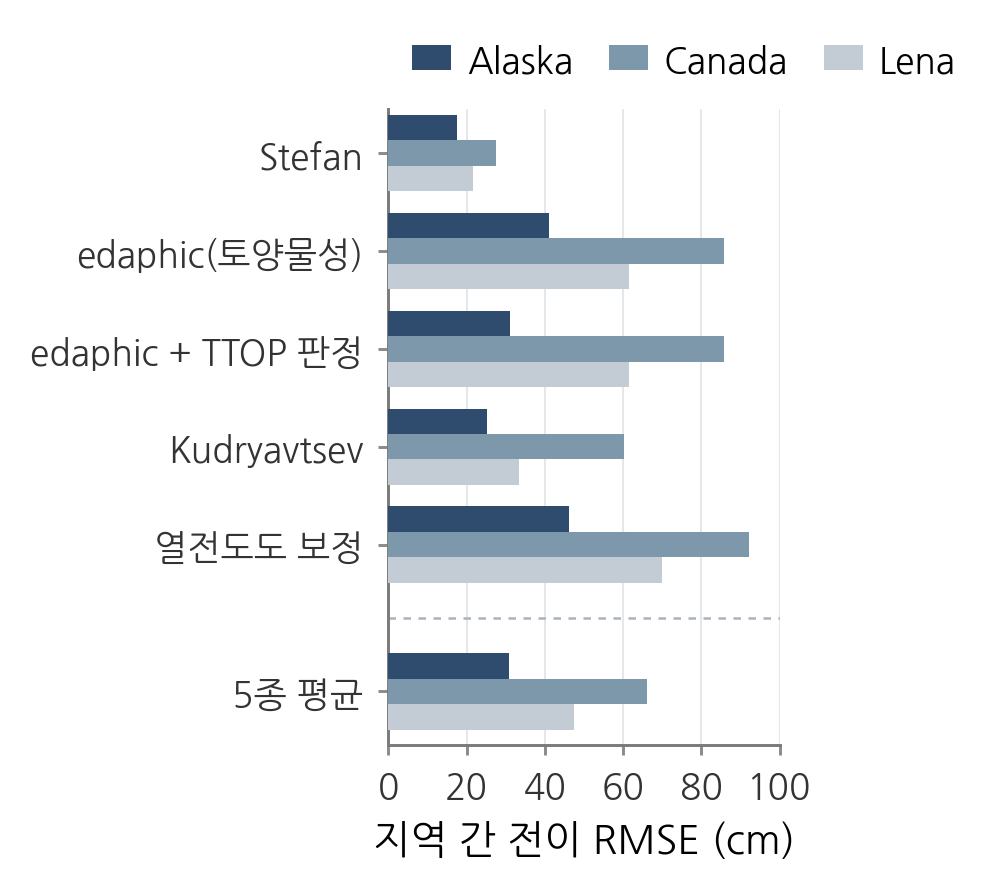
\includegraphics[width=\linewidth]{../figures/s2_physics/physics_loro_bars.png}
  \caption{물리식 5종과 그 평균의 지역별 오차(학습 없이 산출식만 적용, 계수 $E$는 학습 지역 적합, 지역 단위 홀드아웃). Stefan만 전 지역에서 정확하다. edaphic과 TTOP 판정의 막대는 알래스카에서만 갈라지는데, 다른 두 지역은 전 셀이 판정을 통과하기 때문이다.}
  \label{fig:physbars}
\end{subfigure}\hfill
\begin{subfigure}[t]{0.32\textwidth}
  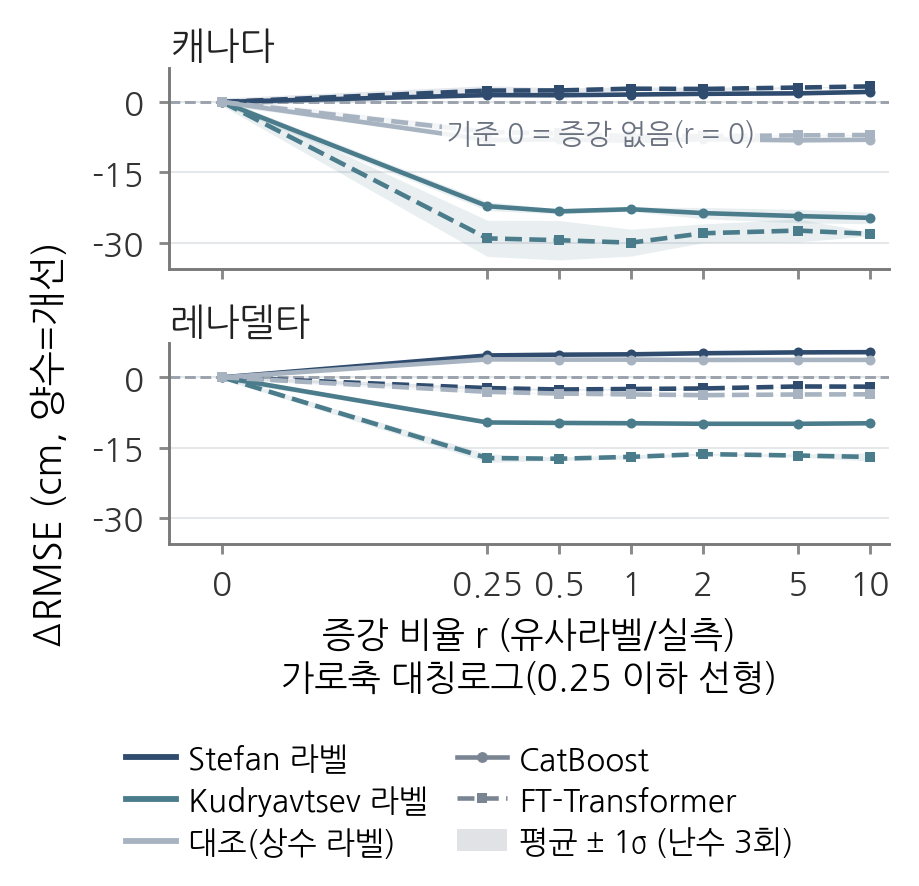
\includegraphics[width=\linewidth]{../figures/s3_aug/aug_response_curves.png}
  \caption{증강 비율 $r$에 따른 반응(학습원=알래스카 실측, 대상 지역은 공변량만 사용, 대상 셀의 절반에 유사라벨 부여 후 나머지 절반의 실측으로 평가). 정확한 물리는 개선, 부정확한 물리는 악화시킨다. 두 패널은 세로축을 공유한다.}
  \label{fig:augcurve}
\end{subfigure}\hfill
\begin{subfigure}[t]{0.32\textwidth}
  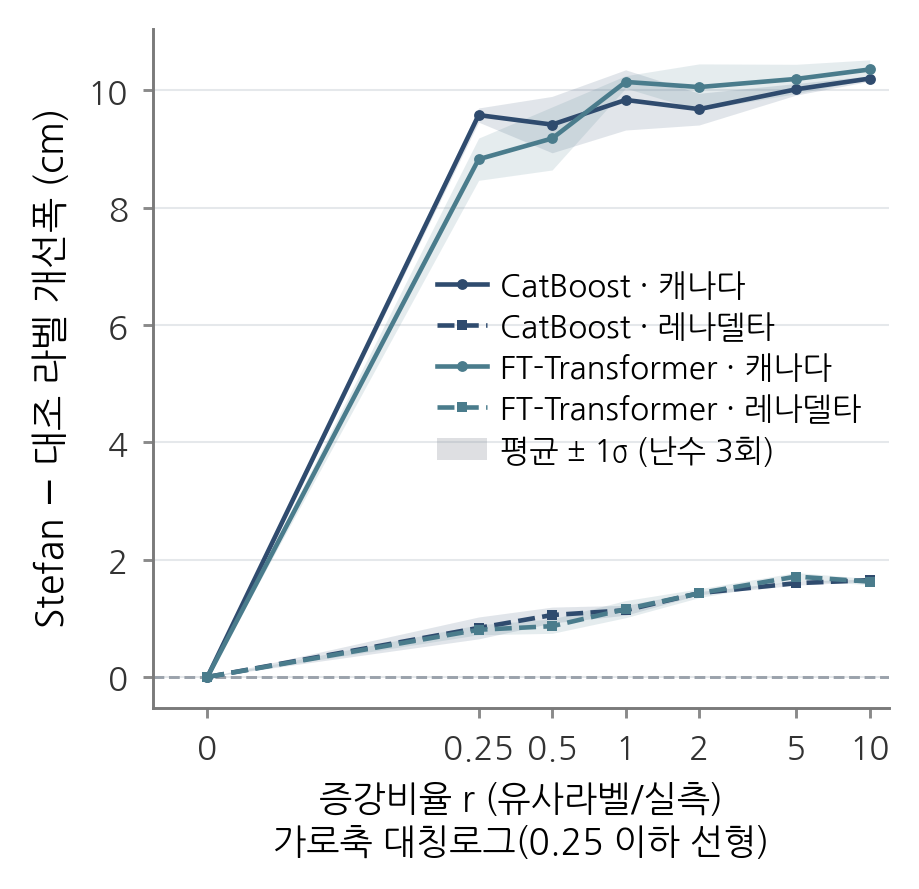
\includegraphics[width=\linewidth]{../figures/s3_aug/physics_net_value.png}
  \caption{물리 정보의 순가치(Stefan 라벨 개선폭 $-$ 대조 라벨 개선폭). 같은 $r$과 같은 난수에서 짝지어 계산하므로 기준항이 상쇄된다. 증강 비율을 키울수록 커진다. 음영은 난수 3회의 $\pm 1\sigma$이다.}
  \label{fig:netvalue}
\end{subfigure}
\caption{물리경험식 비교와 물리 유도 증강의 효과. (a)는 학습 없이 산출식만 쓴 결과, (b,c)는 대상 지역의 공변량은 쓸 수 있고 실측 라벨만 없는 조건이다. 정확한 물리 유사라벨을 데이터 희소 지역에 증강하면 예측이 개선되고, 그 이득이 물리 정보에서 옴을 상수 라벨 대조로 분리한다.}
\label{fig:physaug}
\end{figure*}


\subsection{물리 결합 모델}
\emph{조건: 지역 내(비교를 위해 정보 없음 결과를 함께 제시).}
물리와 기계학습을 결합하면 지역 내 정확도를 더 끌어올릴 수 있다. 식~\eqref{eq:residual}과 같이 Stefan 예측을 기준선으로 두고 능형 회귀로 학습한 잔차를 가중 $\lambda$로 더하면, 알래스카 지역 내에서 $13.33\,\mathrm{cm}$로 본 연구의 최저 오차를 달성한다($\lambda{=}0.75$, 입력 25종). 물리식 단독($14.46$)이나 순수 신경망($14.37$)보다 낮아, 물리가 설명하는 부분과 데이터가 설명하는 부분이 서로 보완됨을 보인다.

다만 이 이득은 학습 지역 안에서만 성립한다(그림~\ref{fig:transfer}(a)). 잔차 모델은 알래스카의 공변량-잔차 관계를 학습하므로, 환경이 다른 지역에 그대로 적용하면 그 관계가 유지되지 않는다. 지역 내 최저를 달성한 설정을 그대로 전이에 적용하면 $35.45\,\mathrm{cm}$로 크게 악화되고, 잔차를 저용량 부스팅으로 바꾸고 가중을 $\lambda{=}0.25$로 낮춘 설정이라야 $21.83\,\mathrm{cm}$로 물리식 단독($21.26$)에 근접한다. 두 검증축의 $\lambda$ 반응은 형태가 다르다. 지역 내 오차는 $\lambda$를 키우면 줄다가 $\lambda\,{\approx}\,0.5\text{--}0.75$에서 최소가 된 뒤 다시 늘어나는 반면, 전이 오차는 $\lambda{=}0$에서 이미 최소이고 이후 단조 증가한다. 지역 내 최적 가중과 전이 최적 가중이 어긋나므로 하나의 $\lambda$로 두 목표를 동시에 만족시킬 수 없다.

\subsection{지역 간 전이}
\emph{조건: 정보 없음. 세 지역 비가중평균.}
관측이 전혀 없는 지역으로 넘어갈 때는 양상이 달라진다(그림~\ref{fig:transfer}(b), 표~\ref{tab:transfer}). 순수 기계학습은 학습 지역의 공변량-ALT 관계를 그대로 적용하므로 환경이 바뀌면 오차가 모델에 따라 $34\text{--}38\,\mathrm{cm}$로 커진다. 공간보간은 좌표만 사용하므로 공간 자기상관 구조가 다른 지역으로는 넘어가지 못한다. 보간 방식에 따라 보통 크리깅 $29.4$, 회귀 크리깅 $36.3$, 역거리가중 $50.9\,\mathrm{cm}$로 벌어진다. 반면 Stefan 식은 기후에서 융해 깊이를 직접 산출하고 그 관계가 지역이 바뀌어도 유지되므로 $21.26\,\mathrm{cm}$를 유지한다.

이 격차를 좁히기 위해 물리 사전학습 후 미세조정, 자료원별 신뢰도를 반영하는 다중충실도 모델, 물리식을 공변량으로 가중 결합하는 혼합 모델을 같은 조건에서 시험하였다. 이 가운데 다중충실도($21.84\,\mathrm{cm}$)와 혼합 모델($29.22$)은 앞 절의 잔차 학습($21.83$)과 함께 그림~\ref{fig:transfer}(b)에 싣는다. 세 구조 모두 물리식 단독을 유의하게 넘지 못하였고, 앞 절의 유사라벨 증강도 지역 단위 홀드아웃으로 옮기면 $21.28\,\mathrm{cm}$로 물리식과 동률이었다(대상 지역의 보조 관측을 학습에 쓰는 설정이라 물리식과 엄밀히 같은 조건은 아니다). 물리 유사라벨은 물리식이 이미 담고 있는 정보를 학습 모델에 옮겨 심는 역할을 하므로, 증강만으로는 물리식 자체를 넘어서기 어렵다. 이는 전이 성능을 끌어올리려면 물리식이 갖지 못한 정보를 추가해야 함을 뜻한다.

\begin{table}[H]
\centering
\footnotesize
\caption{지역 내 대 지역 간 전이 성능(RMSE, cm). 전이는 관측이 전혀 없는 지역을 가정한 지역 단위 홀드아웃이며, 세 지역 오차의 비가중 평균이다. 물리 결합은 설정에 따라 두 행으로 나누어 제시한다. 이 표의 Stefan은 계수 $E$를 최소제곱으로 추정한 값으로, 표~\ref{tab:physics}의 중앙값비 추정보다 지역 내 $0.10$, 전이 $0.98\,\mathrm{cm}$ 낮다.}
\label{tab:transfer}
\begin{tabular}{@{}lrr@{}}
\toprule
\tabhead{방법} & \tabhead{지역 내} & \tabhead{전이} \\
\midrule
Stefan 물리식 & 14.46 & \textbf{21.26} \\
물리 결합(지역 내 최적) & \textbf{13.33} & 35.45 \\
물리 결합(전이 최적) & 13.92 & 21.83 \\
다층 퍼셉트론 & 14.37 & 34.24 \\
CatBoost & 15.61 & 38.42 \\
공간보간(크리깅) & 15.77 & 29.40 \\
\bottomrule
\end{tabular}
\end{table}

\subsection{물리식과 독립 관측의 결합}
\emph{조건: 공변량만과 정보 없음 두 조건을 나란히. 대상은 레나델타·캐나다 두 지역.}
이 절의 수치는 레나델타와 캐나다 두 지역의 평균이며 알래스카를 포함하지 않는다. 입력 집합과 평가 대상도 앞 절과 다르다.

전이 오차를 편향과 산포로 분해하면 오차의 주성분이 편향임이 드러난다. 물리식은 지역마다 서로 다른 방향으로 치우친다. 관측이 전혀 없는 조건에서 레나델타는 평균 $5.5\,\mathrm{cm}$, 캐나다는 $2.3\,\mathrm{cm}$ 과대예측한다. 지역마다 토양 물성과 수분 조건이 달라 단일 계수로는 수준을 맞출 수 없기 때문이다.

여기에 물리식과 산출 방식이 다른 정보를 더할 수 있다. 위성 관측 기반 ALT 제품(ESA CCI[11])은 전 지역에서 확보되며, 위성 지표온도와 적설·토양 자료를 결합해 생산되므로 재분석 기온만으로 계수를 적합하는 Stefan 식과 오차 구조가 다르다. 실제로 이 제품은 레나델타에서 $8.8\,\mathrm{cm}$ 과소, 캐나다에서 $10.6\,\mathrm{cm}$ 과대예측하여, 레나델타에서는 물리식과 부호가 반대이다(그림~\ref{fig:s12}(c)).

두 추정을 동일 가중으로 평균하면 오차가 두 방향에서 줄어든다. 부호가 반대인 경우에는 편향이 직접 상쇄되어 레나델타의 편향이 $+5.5$에서 $-1.5\,\mathrm{cm}$로 작아진다. 부호가 같은 캐나다에서는 편향이 $+2.3$에서 $+6.6\,\mathrm{cm}$로 오히려 커지지만, 두 추정의 오차가 서로 독립이어서 산포 성분이 $27.4$에서 $24.9\,\mathrm{cm}$로 줄고 결과적으로 전체 오차는 낮아진다. 네 개의 지역·조건 조합 모두에서 오차가 감소하며, 편향의 크기가 줄어드는 경우는 그중 셋이다.

이 결합을 앵커로 두고 그 위에 작은 가중의 잔차 모델을 더하는 구성을 체계적으로 탐색하였다. 앵커·유사라벨·증강 비율·잔차 모델의 185개 조합을 만들고 각 조합에 잔차 가중 5단계를 적용하여 두 조건에서 평가하였다(표~\ref{tab:s12}, 그림~\ref{fig:s12}). 관측이 전혀 없는 조건에서 두 지역 평균 오차는 물리식 단독 $24.60$에서 결합 앵커 $23.27$, 잔차를 더한 구성에서 $22.92\,\mathrm{cm}$로 낮아진다. 대상 지역 공변량을 쓸 수 있는 조건에서는 $23.72$에서 $21.32\,\mathrm{cm}$까지 낮아진다.

탐색 결과에서 세 가지 규칙성이 확인된다. 상위 구성은 거의 전부 물리식과 CCI 제품을 함께 앵커로 삼았고, 개선의 주된 원천은 편향 상쇄였다. 각 $\lambda$에서 최선 구성을 취하면 두 조건 모두 $\lambda{=}0.25$에서 가장 낮고 그 이상에서는 다시 나빠지는데(그림~\ref{fig:s12}(d)), 잔차를 크게 반영하면 학습 지역의 공변량-잔차 관계가 대상 지역으로 과하게 옮겨지기 때문이다. 앵커와 유사라벨 증강은 물리식·위성 제품이 담은 같은 보조 정보를 각각 예측 단계와 학습 단계에서 주입하는 두 경로이며, 어느 쪽이 더 기여하는지는 조건에 따라 달라진다. 대상 지역 공변량을 쓸 수 있는 조건의 최상위 구성은 두 경로를 함께 사용하였고(물리 앵커 + 위성 유사라벨), 관측이 전혀 없는 조건의 최상위 구성에는 증강이 포함되지 않았다.

다만 개선폭의 통계적 유의성은 확정하지 못하였다. 짝지은 블록 부트스트랩에서 물리식 단독 대비 결합 앵커의 오차 감소는 두 지역 평균 $0.62\,\mathrm{cm}$이고 $95\%$ 신뢰구간이 $-2.22$에서 $+2.76$까지 걸쳐 $0$을 포함한다. 신뢰구간이 $0$을 포함한다는 것은, 평가에 쓰인 공간블록을 다시 뽑았을 때 개선이 사라지거나 부호가 뒤집히는 경우도 배제할 수 없다는 뜻이다. 원인은 평가 단위가 되는 공간블록이 지역당 $11\text{--}30$개로 적다는 데 있다. 블록이 적으면 재표집마다 결과가 크게 흔들려 작은 개선을 통계적으로 가려낼 수 없다. 오차 감소는 네 조합 모두에서 같은 방향으로 나타나므로, 본 연구는 이를 확정된 성능 향상이 아니라 재현 가능한 경향으로 제시한다.

\begin{table}[H]
\centering
\footnotesize
\caption{물리식과 CCI 제품의 결합 효과(레나델타·캐나다 두 지역 평균 RMSE, cm). 앞 열은 대상 지역의 공변량만 학습에 쓸 수 있는 조건, 뒤 열은 대상 지역의 공변량과 라벨을 모두 쓸 수 없는 조건이다.}
\label{tab:s12}
\begin{tabular}{@{}lrr@{}}
\toprule
\tabhead{방법} & \tabhead{대상 공변량 사용} & \tabhead{대상 정보 없음} \\
\midrule
기계학습 단독(CatBoost) & 27.94 & 26.61 \\
위성 제품 단독 & 25.90 & 26.27 \\
물리식 단독 & 23.72 & 24.60 \\
물리식+위성 제품 & 21.68 & 23.27 \\
\quad + 잔차 학습 & \textbf{21.32} & \textbf{22.92} \\
\bottomrule
\end{tabular}
\end{table}


\begin{figure*}[!t]
\centering
\begin{subfigure}[t]{0.5\textwidth}
  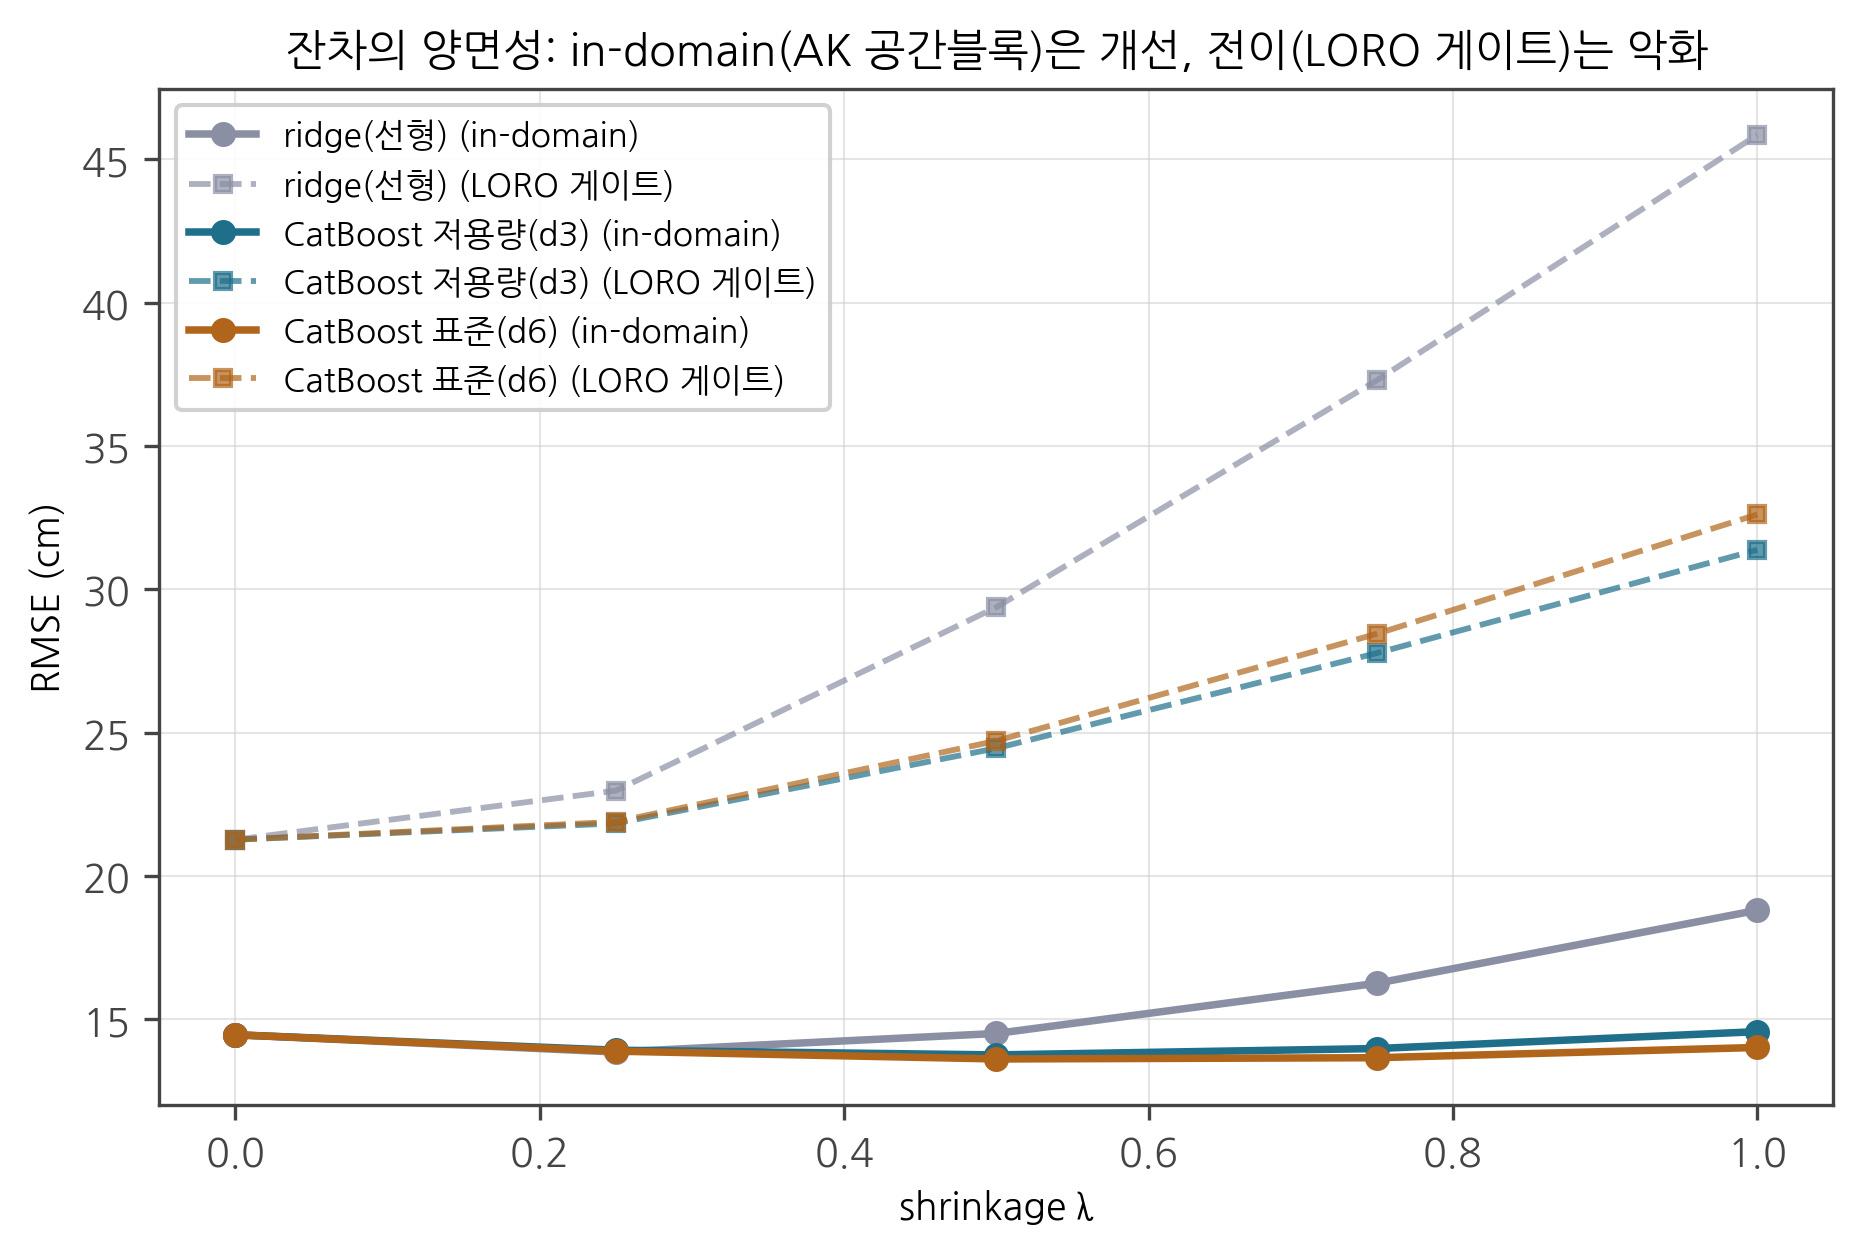
\includegraphics[width=\linewidth]{../figures/s4_residual/s4_indomain_vs_transfer.png}
  \caption{물리 결합 모델(Stefan 앵커 + 잔차 학습, 입력 14종)의 잔차 가중 $\lambda$에 대한 반응. $\lambda$는 Stefan 기준선에 더하는 잔차의 반영 정도이며, $\lambda{=}0$은 물리식 단독이다. 잔차 모델은 능형 회귀와 CatBoost(저용량·표준) 세 계열이고, 실선·채운 표식은 지역 내(알래스카 공간블록 교차검증), 파선·빈 표식은 지역 간 전이(세 지역 홀드아웃의 비가중평균)이다. 전이 곡선의 오차막대는 지역 간 표준오차($n{=}3$)이며, 지역 내 곡선의 시드 간 표준편차는 $0.3\,\mathrm{cm}$ 미만으로 표식보다 작다. 지역 내 곡선은 중간 $\lambda$에서 최소를 지나 다시 오르는 반면 전이 곡선은 $\lambda{=}0$부터 단조 증가하여, 두 목표의 최적 가중이 어긋난다. 본문의 최저 오차 $13.33\,\mathrm{cm}$는 입력 25종에서 얻은 값이므로 본 그림과 직접 비교하지 않는다.}
  \label{fig:s4}
\end{subfigure}\hfill
\begin{subfigure}[t]{0.47\textwidth}
  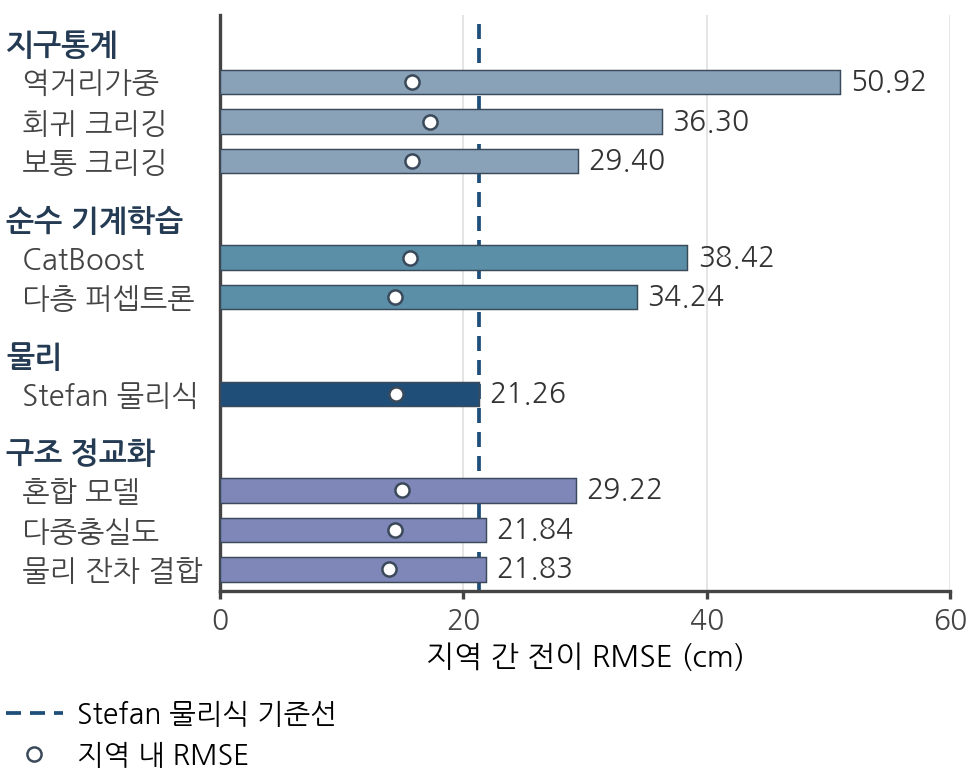
\includegraphics[width=\linewidth]{../figures/02_evaluation/transfer_loro_summary.png}
  \caption{전 접근법의 지역 간 전이 성능(관측이 전혀 없는 지역을 가정한 지역 단위 홀드아웃, 세 지역 비가중평균). 막대는 전이 RMSE, 흰 원은 같은 방법의 지역 내 RMSE(알래스카 공간블록 교차검증)이다. 물리 유도 예측이 순수 데이터 모델보다 견고하다.}
  \label{fig:transfersum}
\end{subfigure}
\caption{물리 결합의 정확도와 지역 간 전이 견고성.}
\label{fig:transfer}
\end{figure*}

\begin{figure*}[!t]
\centering
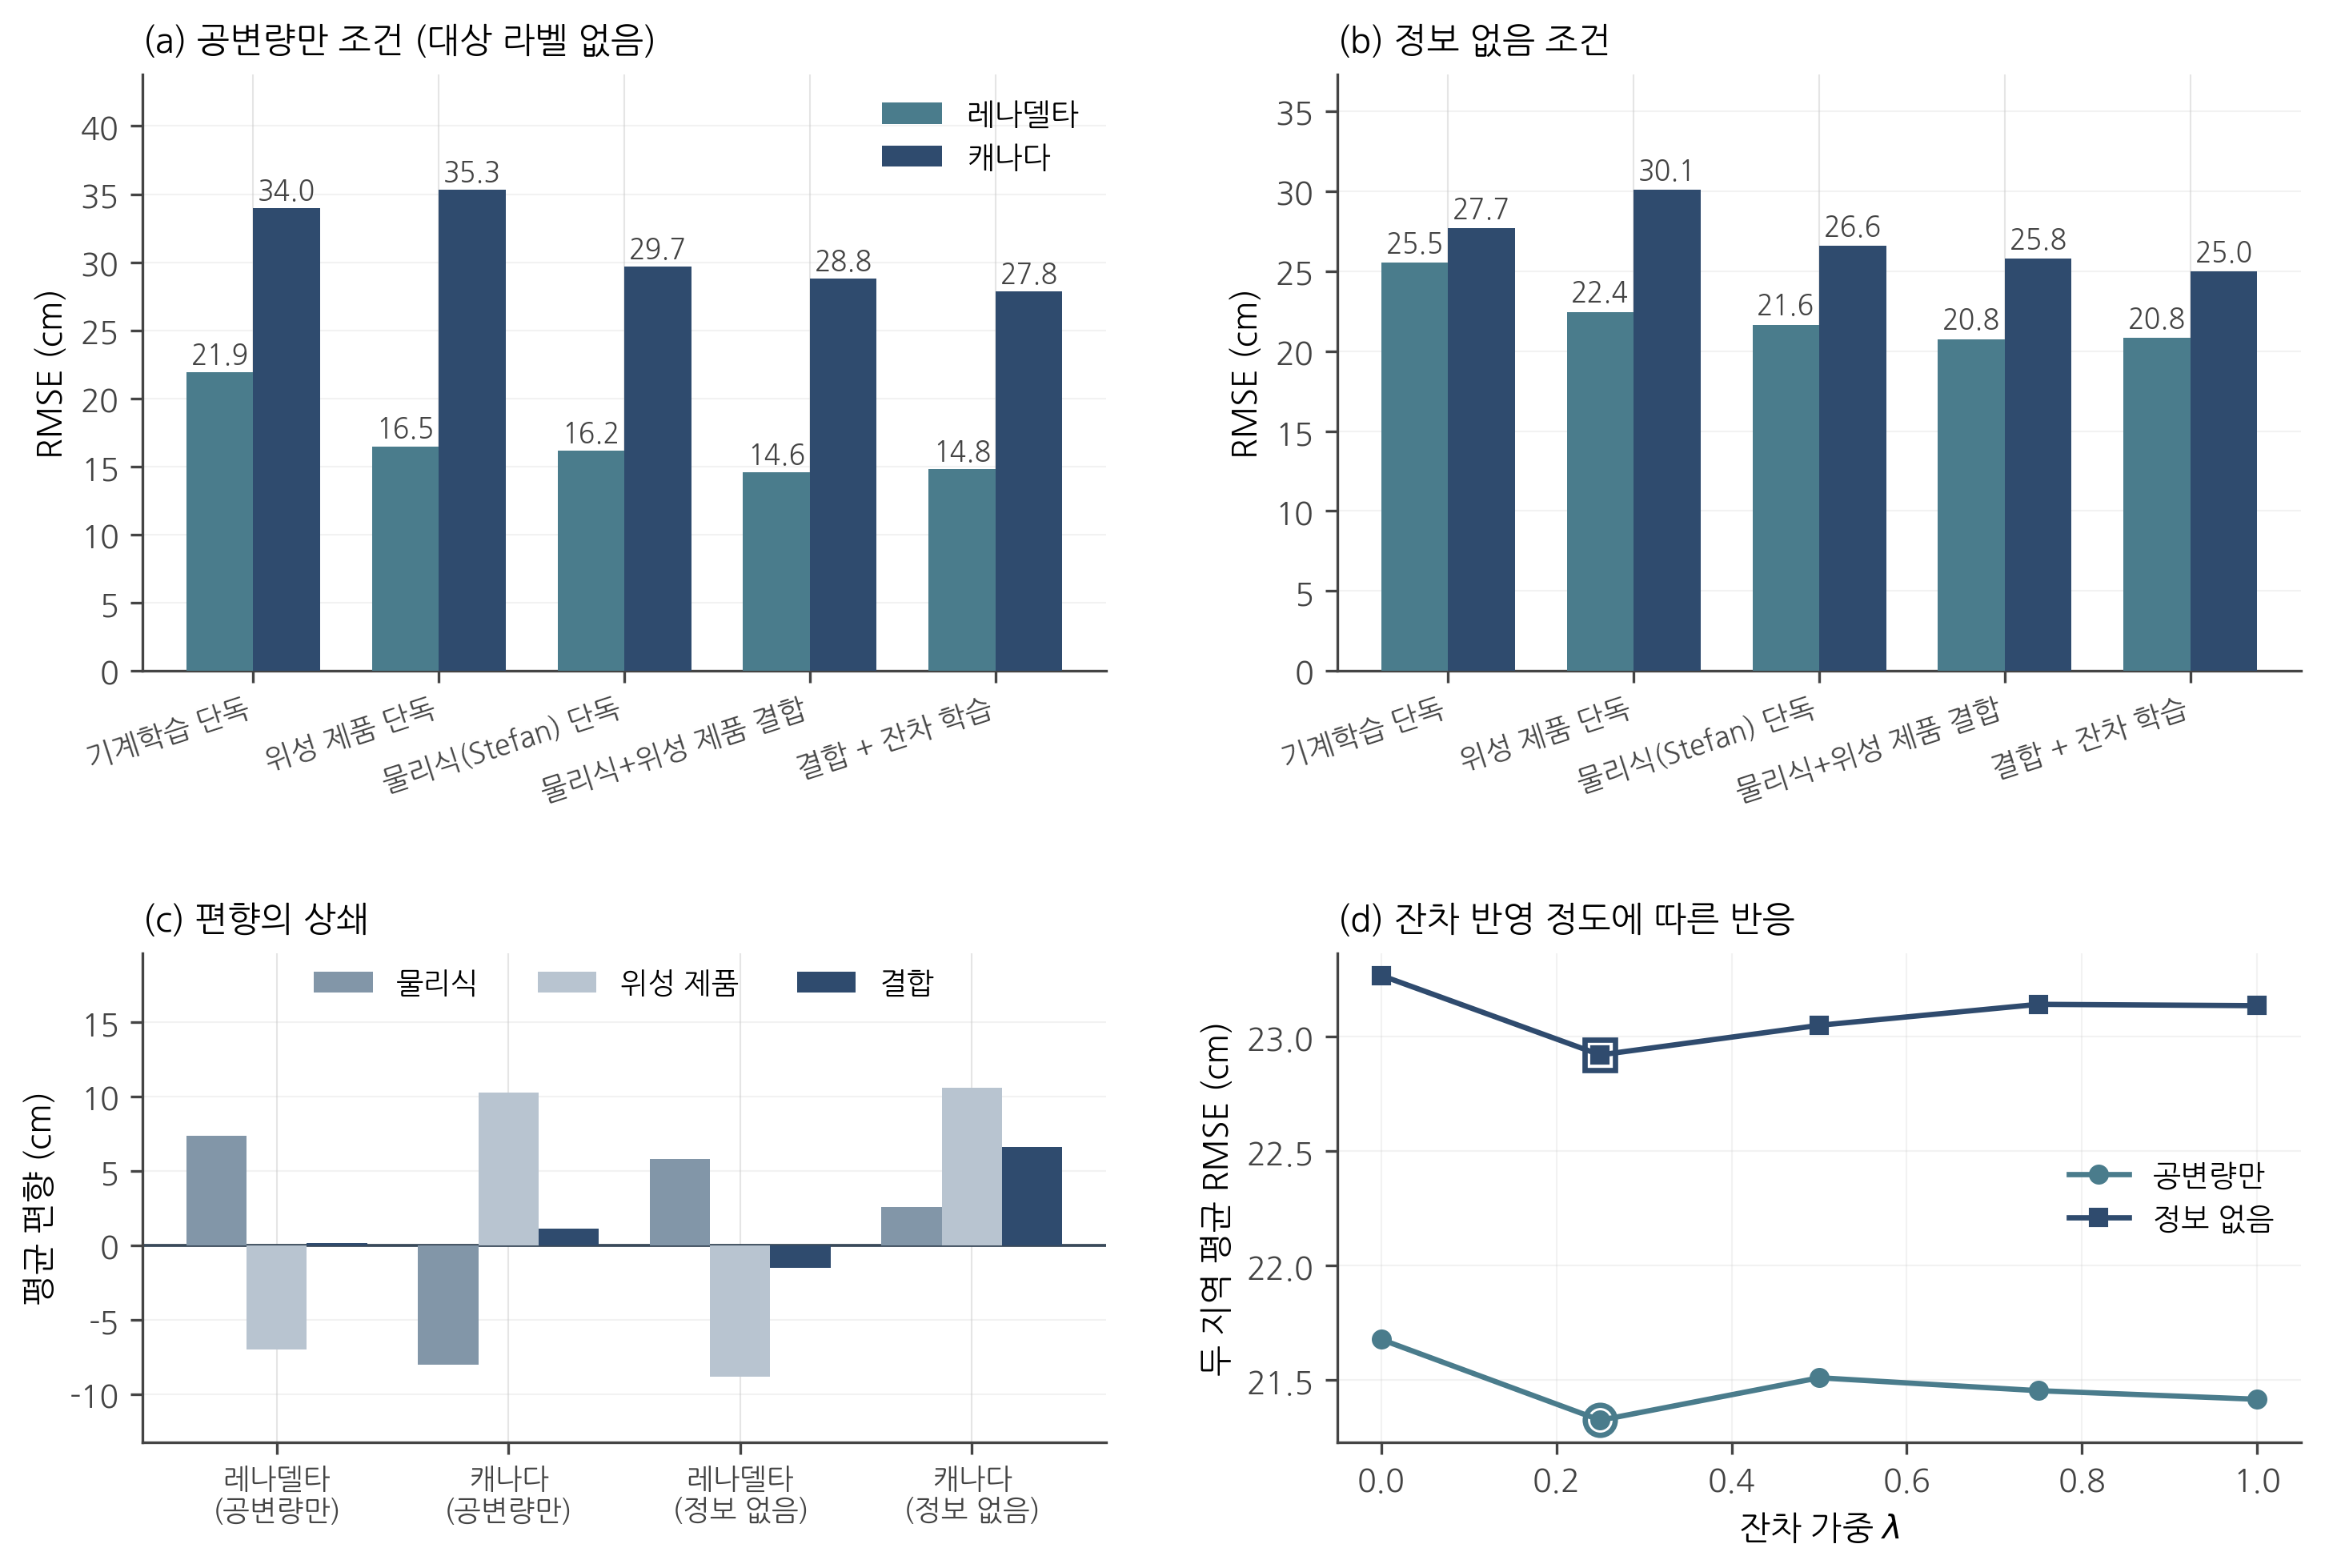
\includegraphics[width=0.88\textwidth]{../figures/s12_hybrid/s12_hybrid_summary.png}
\caption{물리식과 독립 관측의 결합(대상=레나델타·캐나다, 학습원=알래스카 실측, 입력 25종). (a) 대상 지역 공변량을 쓸 수 있는 조건과 (b) 관측이 전혀 없는 조건에서 방법 계열에 따른 지역별 오차이며, 두 패널의 두 지역 평균이 표~\ref{tab:s12}의 두 열이다. (c) 물리식과 위성 제품의 편향이 서로 반대 부호이며 결합 시 상쇄된다. (d) 각 잔차 가중 $\lambda$에서 두 지역이 모두 산출된 구성 중 최소 오차. 빈 표식이 최소점이며 두 조건 모두 $\lambda{=}0.25$이다. $\lambda{=}0$ 값은 (a,b)의 `물리식+위성제품 결합' 행과 같다.}
\label{fig:s12}
\end{figure*}


\subsection{시계열 ALT, 표층 3차원 지중온도장, 계절 융해}
세 공간 산출물은 서로 다른 라벨과 검증축을 가진 병렬 모델이며 하나의 연쇄가 아니다. 앞 절의 ALT 지도는 셀 단위로 집계한 다년평균 ALT를 대상으로 정적 공변량을 학습한 결과이고, 아래의 두 산출물은 각각 별도의 라벨로 학습하였다.

\textbf{연별 ALT 지도.} 관측을 (위치, 연도) 패널 99{,}931행으로 재구성하고, 그해의 기후 입력만으로 ALT를 예측하는 모형들을 연도 홀드아웃으로 비교하였다. Stefan 형태의 2모수 회귀가 $14.97\,\mathrm{cm}$로 부스팅($19.19$)과 다층 퍼셉트론($16.27$)보다 낮아 이를 채택하고 2010--2024년 지도를 생성하였다(그림~\ref{fig:s9}). 이 값은 점 단위 패널의 연도 홀드아웃 결과이므로 셀 집계 기준인 앞 절 수치와 직접 비교하지 않는다. 연도 간 지도 차이는 그해 기후의 반영이며, 같은 지점의 해마다의 변동 자체는 상관 $0.06$으로 예측 신호가 약하다.

\textbf{표층 3차원 지중온도장.} 시추공 깊이별 연최대 지온 764행을 라벨로, 공변량과 깊이 특징을 입력하여 깊이에 따라 단조 감소하도록 제약한 모델을 학습하였다. 온도장 자체는 RMSE $2.66^\circ\mathrm{C}$($R^2\,0.47$)로 재현되어 남북 열구배와 $0^\circ\mathrm{C}$ 등온면의 공간 구조를 보인다(그림~\ref{fig:s10}). 다만 이 온도장에서 $0^\circ\mathrm{C}$ 교차로 유도한 융해 깊이는 실측 대비 $23.8\,\mathrm{cm}$(n=12)로 앞 절의 직접 ALT 예측보다 오차가 크다. 따라서 온도장은 ALT의 대체 산출 경로가 아니라 열구조의 공간 형태를 보이는 결과로 사용한다.

\textbf{계절 내 융해 진행.} $D(t)$는 콘슬 일별 지중온도에서 표층과 연결된 $0^\circ\mathrm{C}$ 등온선으로 유도하였다(그림~\ref{fig:e2row}). $D(t)$는 강한 시간 자기상관을 보여, 7일 전 값을 그대로 쓰는 지속 예측이 $17.5\,\mathrm{cm}$로 가장 정확하다. 반면 누적 융해도일 기반 Stefan($40.8$)과 순환신경망($46.6$)은 이를 넘지 못한다. 2년의 짧은 관측과 지점 수의 제약으로 계절 곡선의 형태를 학습하기에는 표본이 부족한 것으로 판단된다. 계절 내 융해가 예측 가능한 구조를 가진다는 점은 확인되었으나, 현재 확인되는 예측력의 원천은 시간 지속성이다.


\begin{figure*}[!t]
\centering
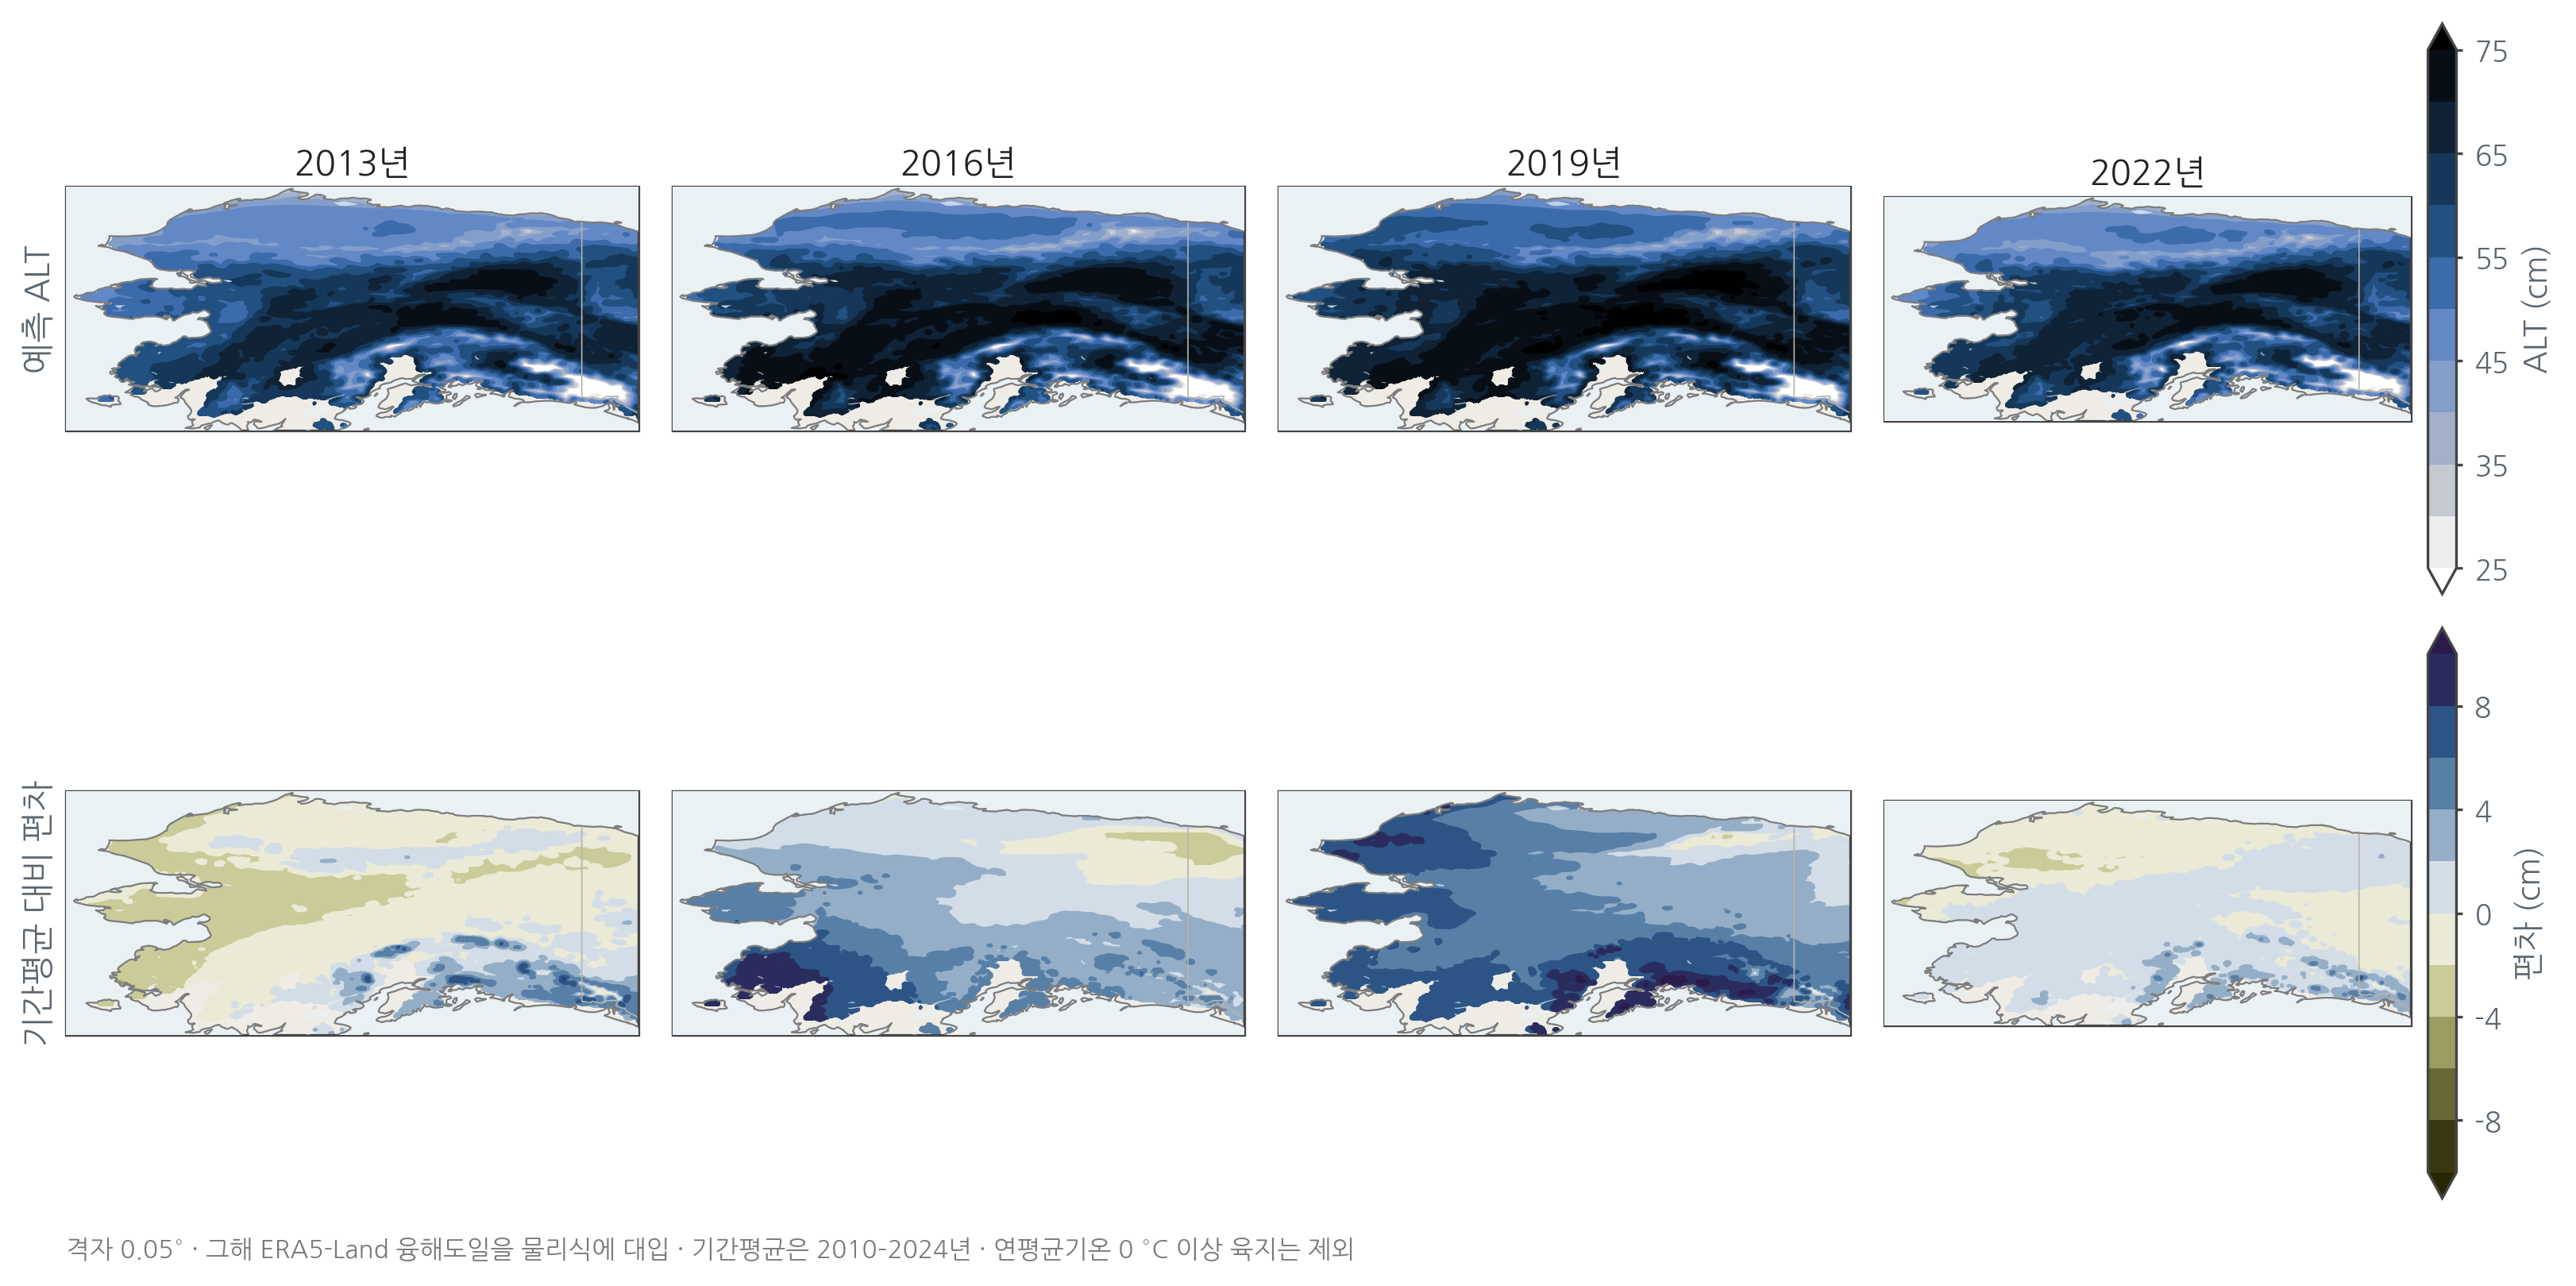
\includegraphics[width=0.94\textwidth]{../figures/s9_timelapse/alt_annual_fields.png}
\caption{연별 ALT 예측장(알래스카, $0.05^\circ$ 격자). 모델은 물리식 단독, 계수 $E$는 알래스카 실측 최소제곱, 영구동토 판정은 연평균기온 $<0^\circ\mathrm{C}$로 그림~\ref{fig:hires}과 같다. 다만 기후값 기간이 2010--2024년으로 그림~\ref{fig:hires}(2015--2020년)과 달라 마스크 경계에 차이가 있다. 위 행은 그해 ERA5-Land 융해도일을 식~\eqref{eq:stefan}에 대입한 절대값, 아래 행은 2010--2024년 평균 대비 편차이다. 2019년은 전역에서 평년보다 깊고 2013년은 얕아, 그해 기후의 공간 구조가 그대로 반영된다.}
\label{fig:s9}
\end{figure*}



\begin{figure*}[!t]
\centering
\begin{subfigure}[t]{0.33\textwidth}
  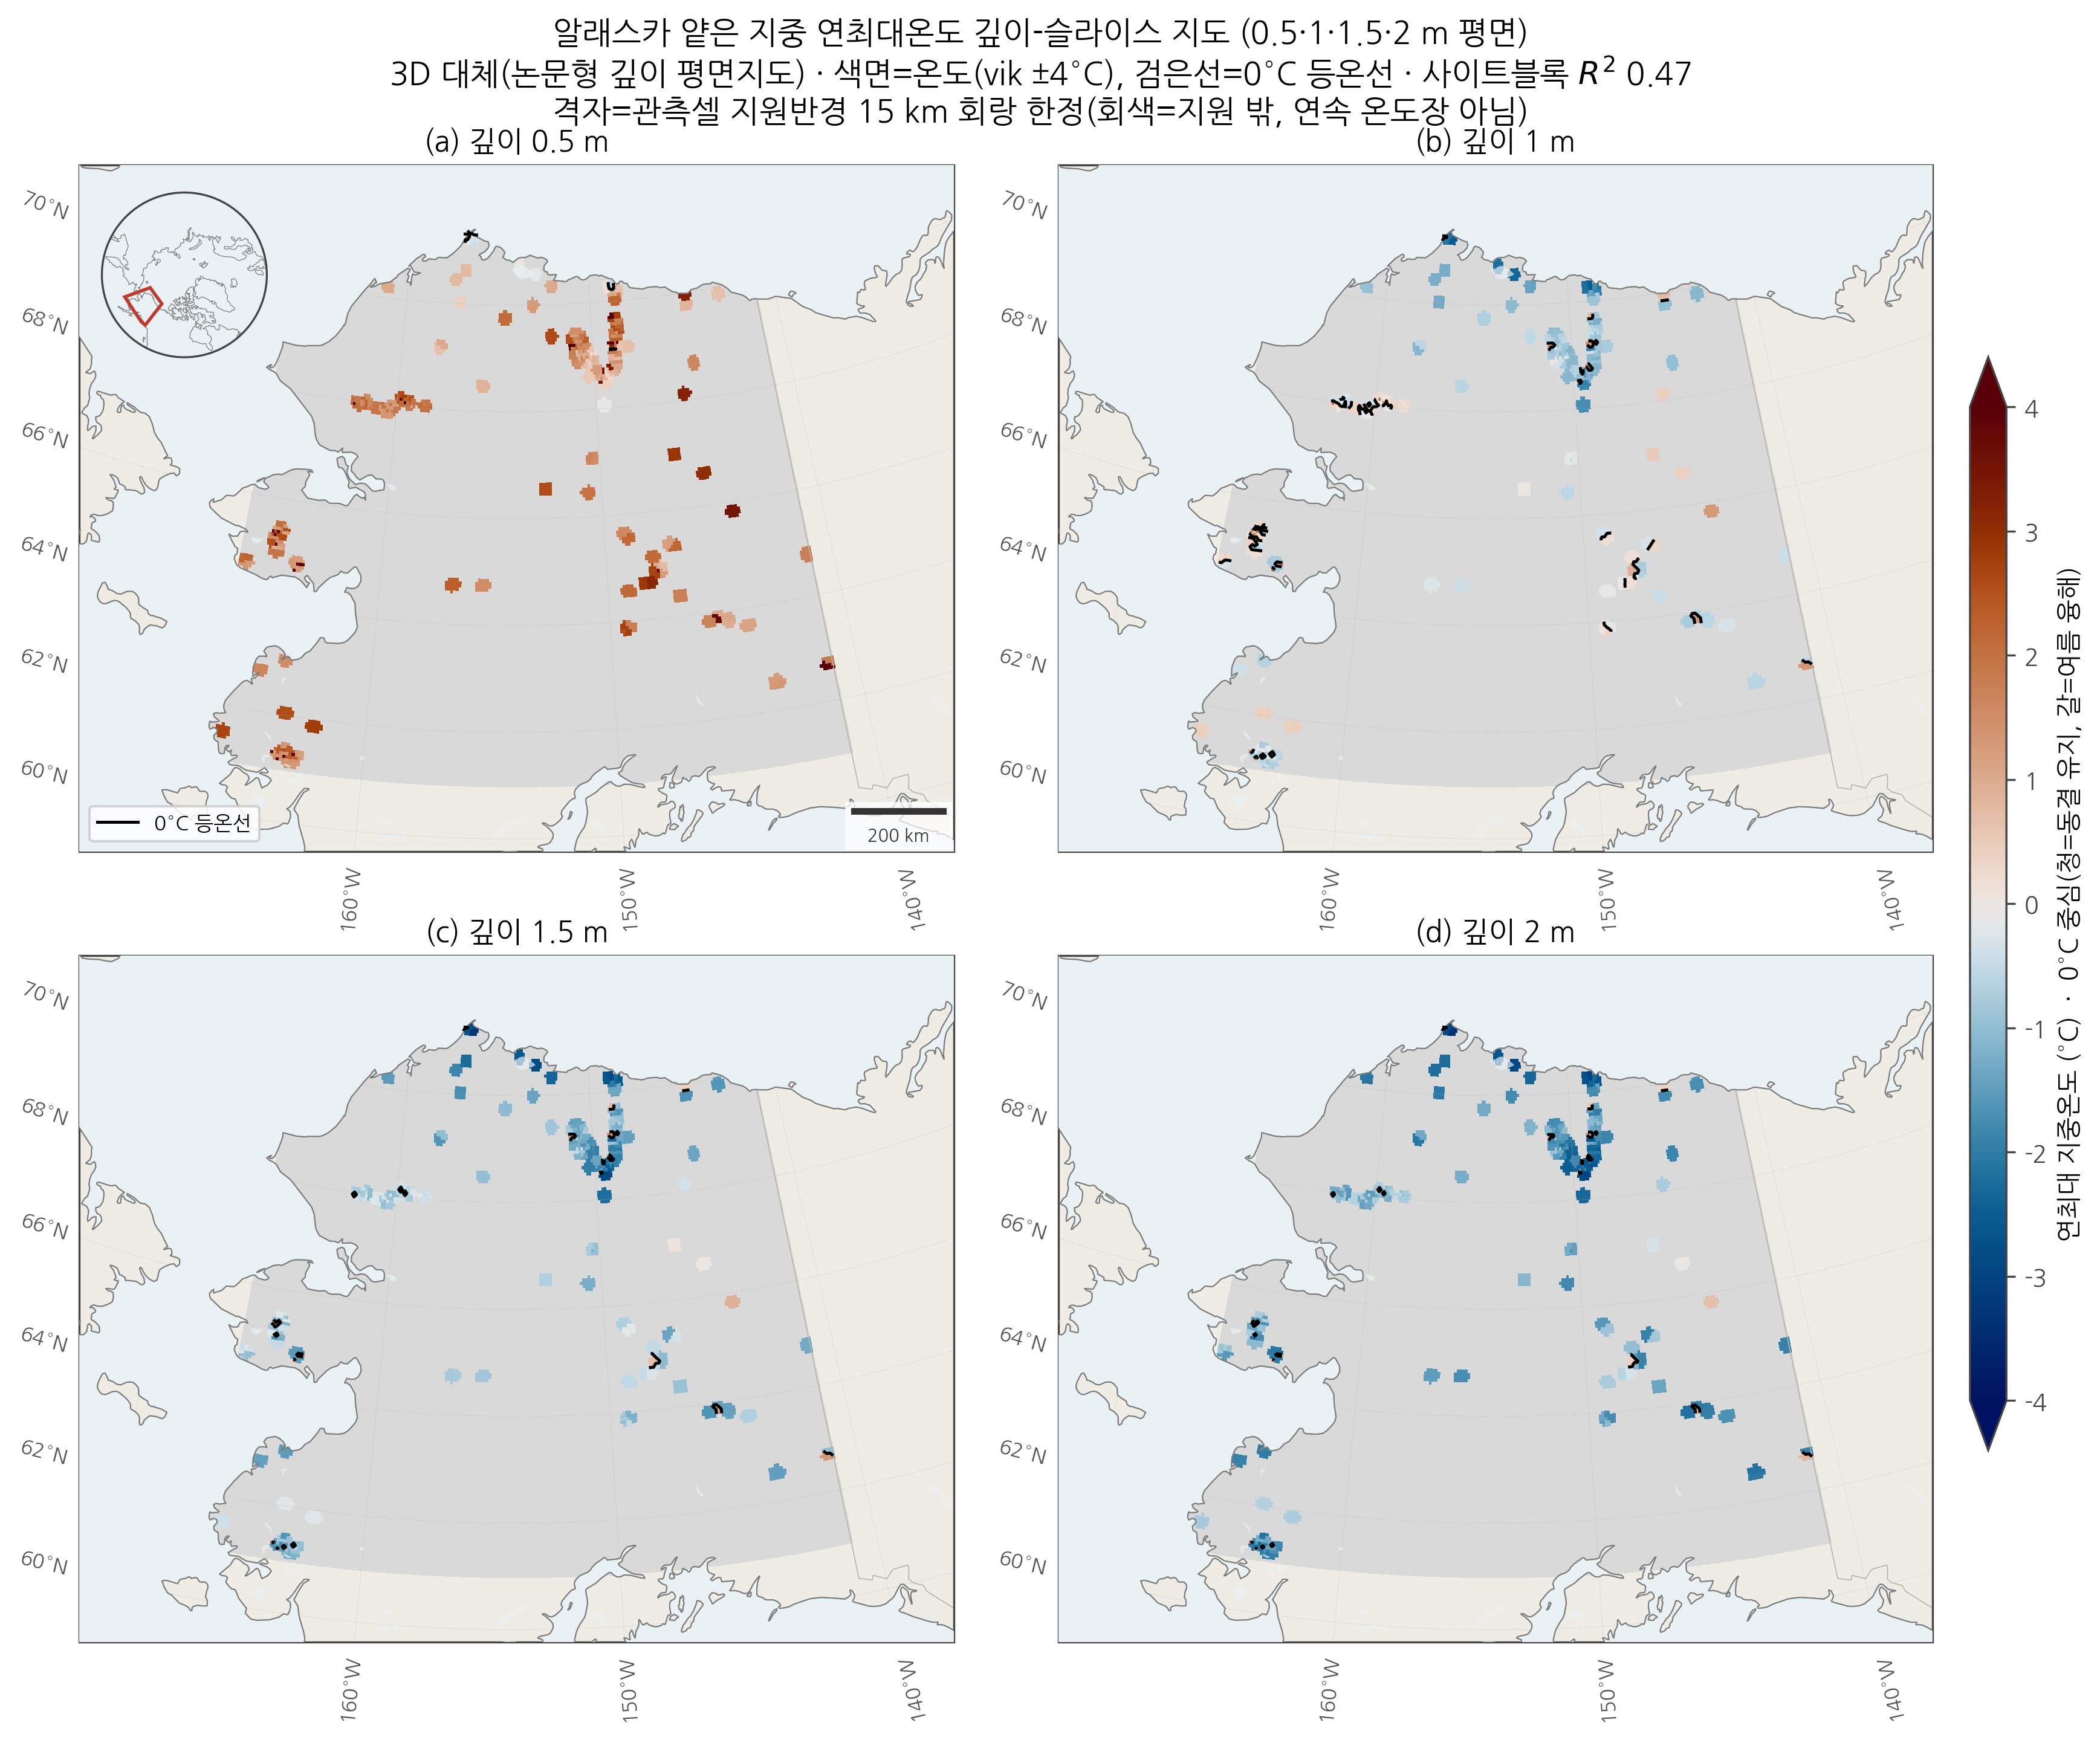
\includegraphics[width=\linewidth]{../figures/s10_shallow3d/s10_depth_slices.png}
  \caption{표층 3차원 지중온도장의 깊이별 슬라이스($0\text{--}3\,\mathrm{m}$). 시추공 깊이별 연최대 지온 764행을 라벨로 학습한 깊이 단조 제약 모델의 예측이며, 검증은 시추공 단위 홀드아웃(RMSE $2.66^\circ\mathrm{C}$)이다. 색은 연최대 지온이며 $0^\circ\mathrm{C}$에서 색이 바뀐다.}
  \label{fig:s10}
\end{subfigure}\hfill
\begin{subfigure}[t]{0.32\textwidth}
  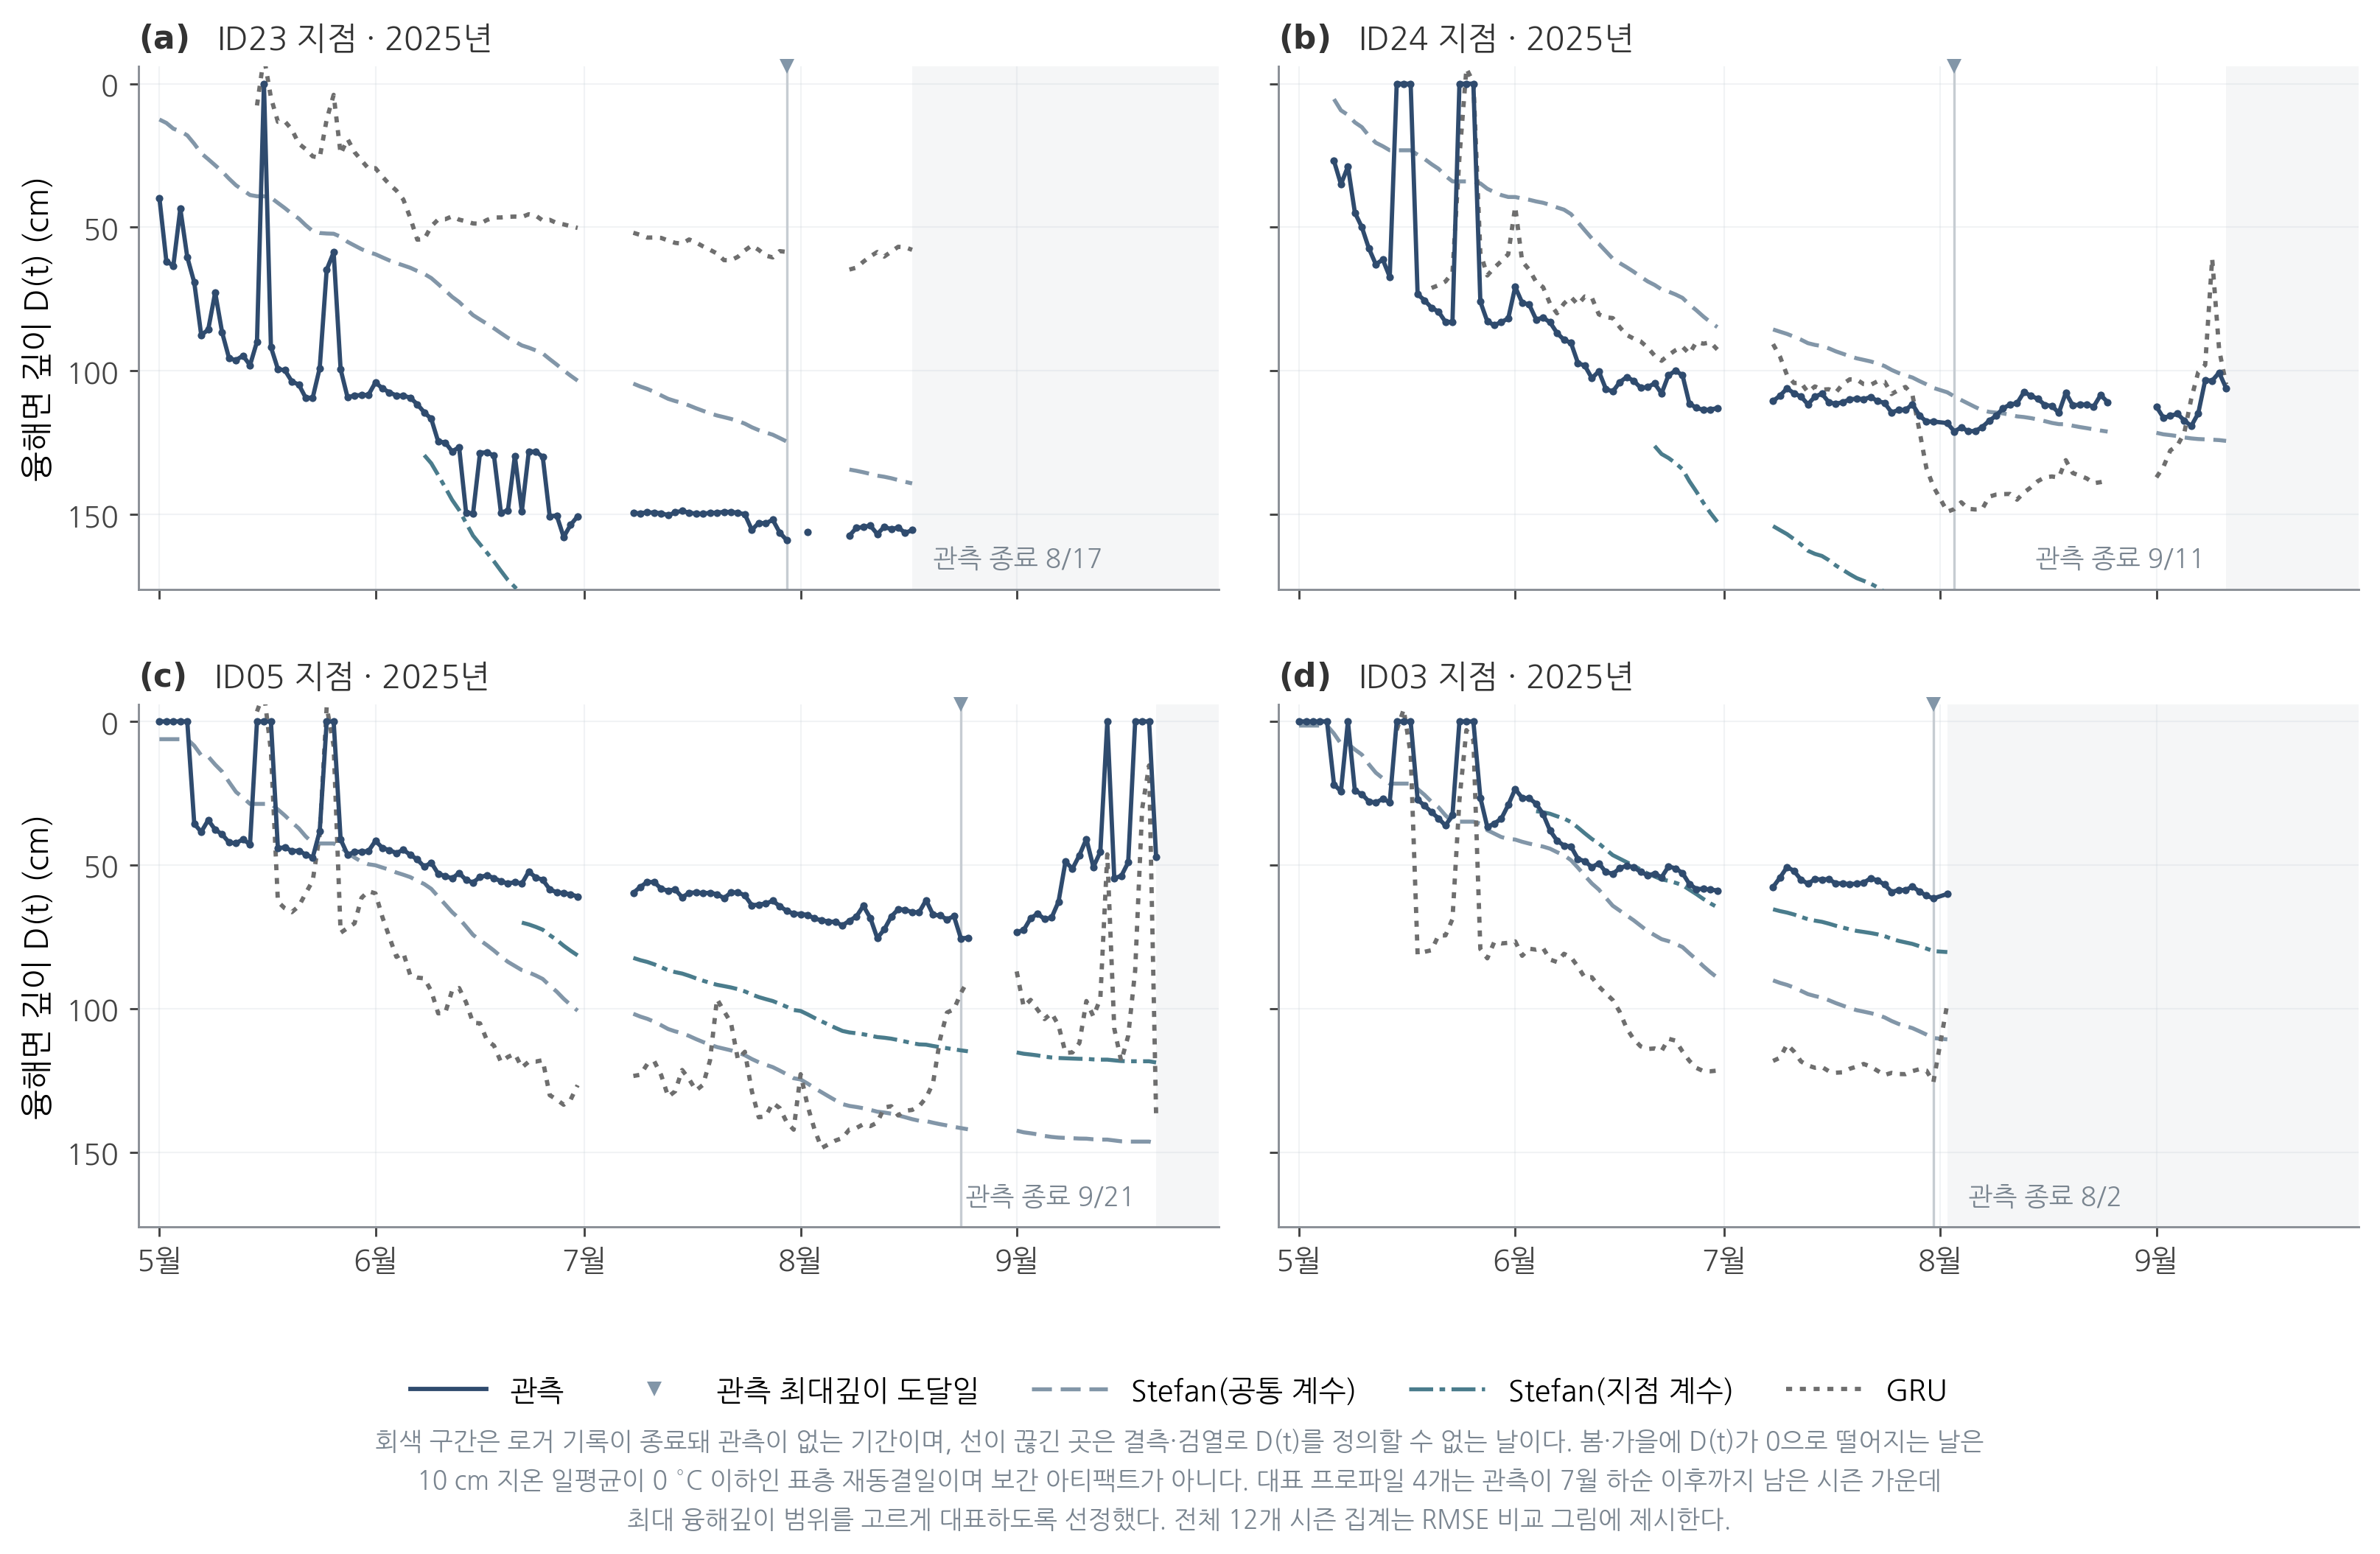
\includegraphics[width=\linewidth]{../figures/e2_seasonal_dt/e2_dt_curves.png}
  \caption{계절 내 융해 진행 $D(t)$의 관측·Stefan·순환신경망 곡선. 라벨은 콘슬 일별 지중온도에서 유도한 $0^\circ\mathrm{C}$ 등온선 깊이이며, 검증축은 지점 홀드아웃과 연도 홀드아웃 두 가지이다. 계절 구조는 예측 가능하다.}
  \label{fig:e2}
\end{subfigure}\hfill
\begin{subfigure}[t]{0.32\textwidth}
  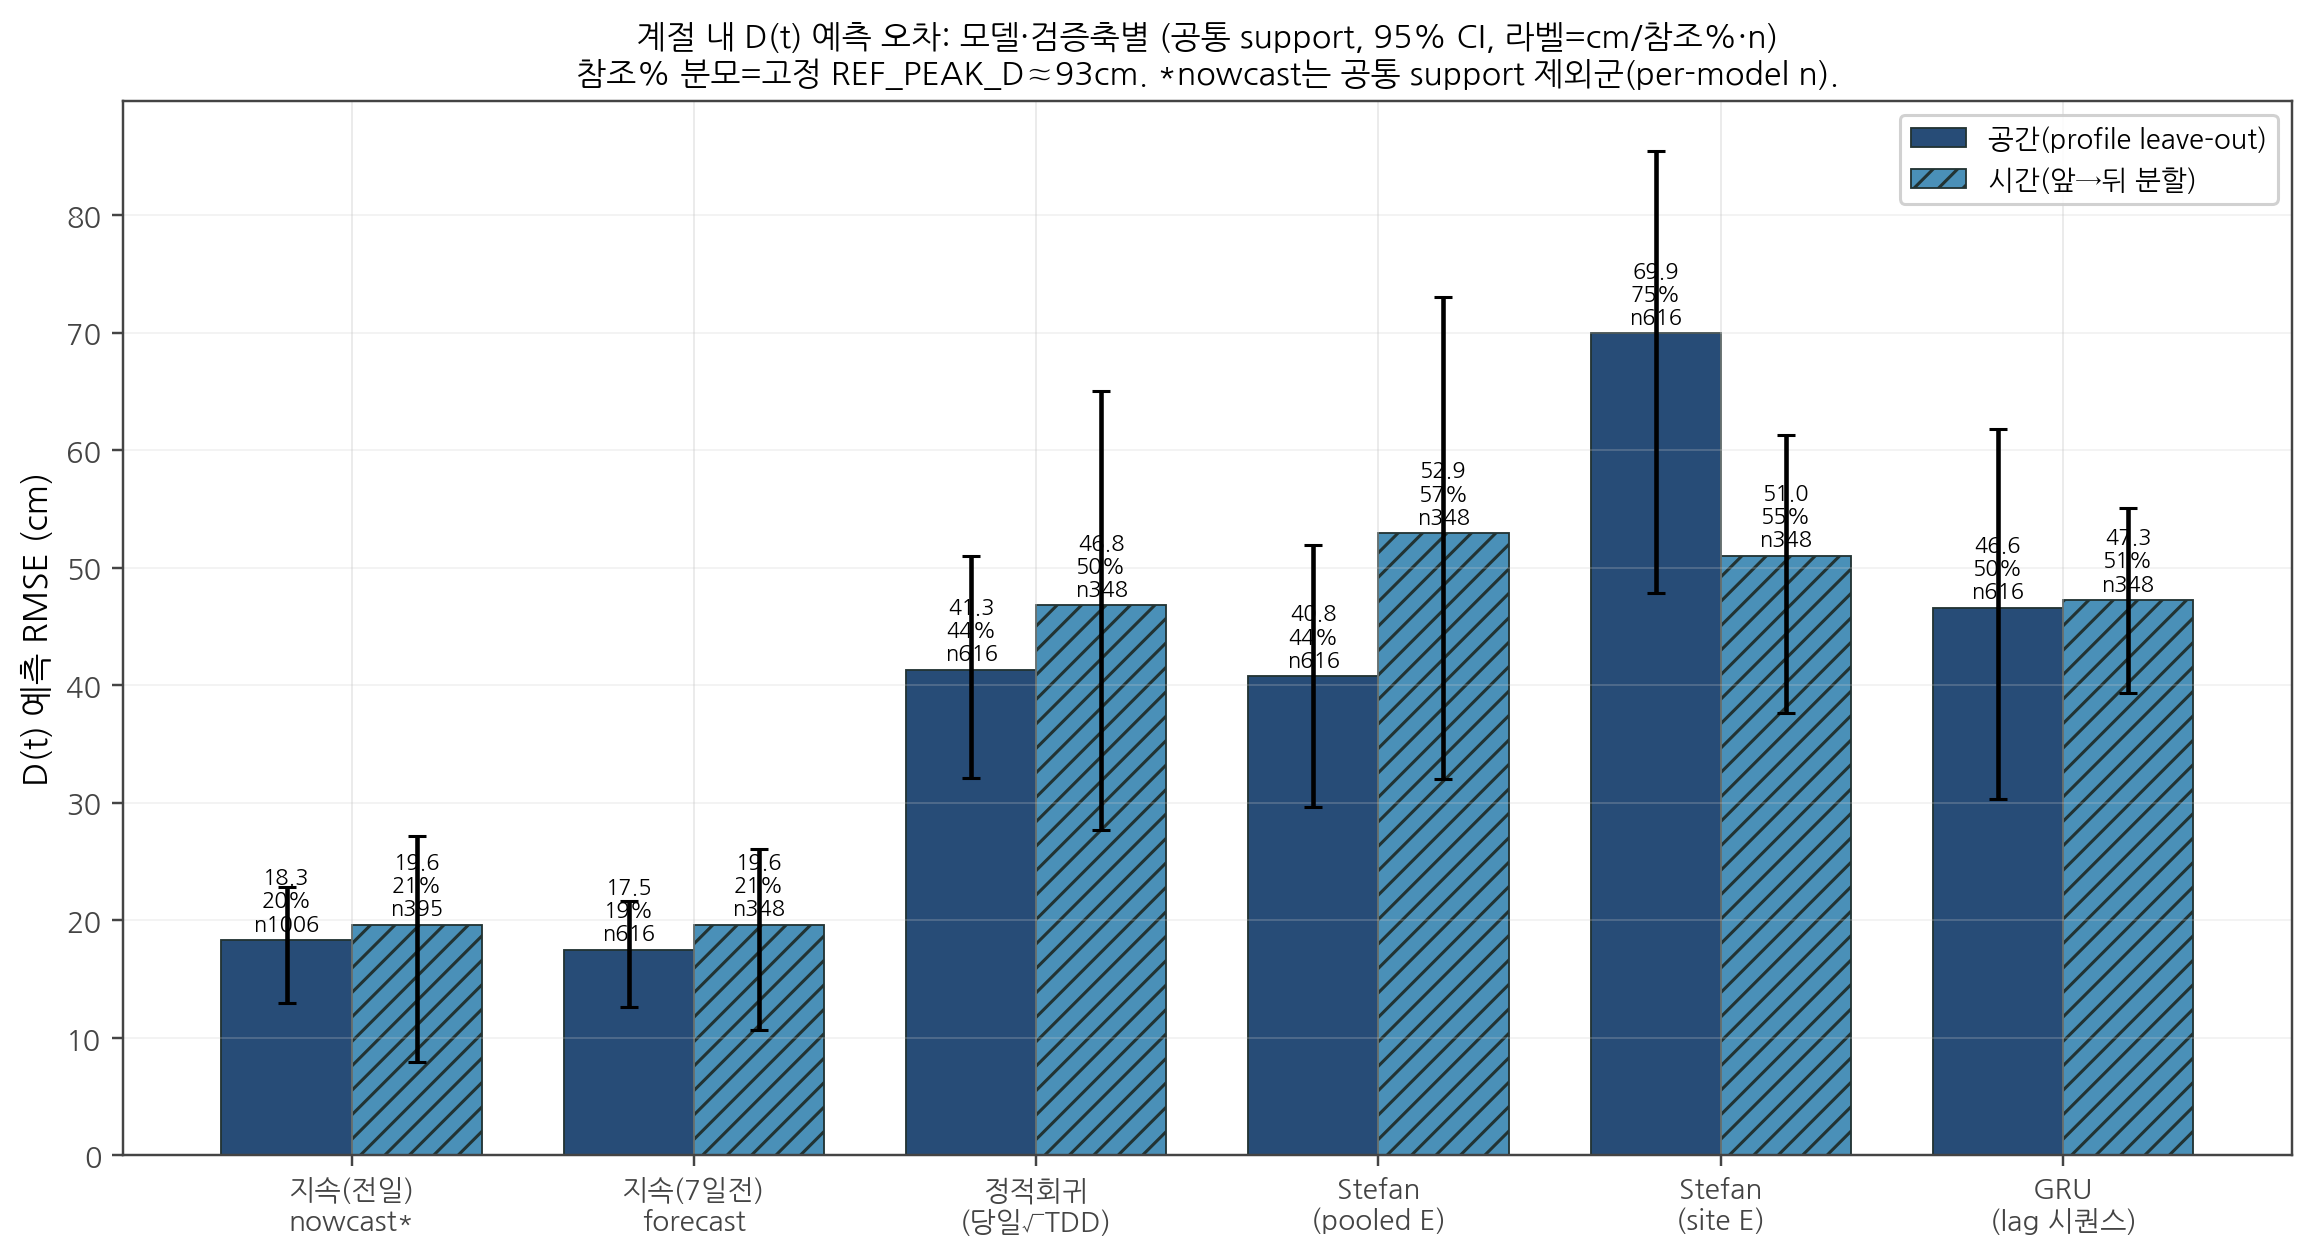
\includegraphics[width=\linewidth]{../figures/e2_seasonal_dt/e2_rmse_bars.png}
  \caption{$D(t)$ 예측 오차 비교. 지속 예측(7일 전 값 그대로), 누적 융해도일 기반 Stefan, 순환신경망을 공간(지점 홀드아웃)·시간(연도 홀드아웃) 두 검증축에서 비교한다.}
  \label{fig:e2bars}
\end{subfigure}
\caption{표층 3차원 지중온도장과 계절 내 융해 진행 $D(t)$.}
\label{fig:e2row}
\end{figure*}


\subsection{보정 불확실성과 KPDC 현장 검증}
\label{sec:kpdc}
예측이 실무에 쓰이려면 신뢰 범위가 필요하다. 분위 회귀의 원 예측구간은 목표 $90\%$ 구간의 실제 포함 비율(커버리지)이 $44.6\%$에 그쳐 과신한다. 식~\eqref{eq:cqr}의 등순응 보정을 적용하면 커버리지가 $93.4\%$로 회복된다(그림~\ref{fig:uq}(a)). 대신 구간 폭이 $14.7$에서 $53.6\,\mathrm{cm}$로 넓어지는데, 이는 관측 표준편차의 약 3배이며, 현재 공변량이 담는 정보량의 한계를 반영한다. 적용가능 영역 분석에서는 학습 분포에서 멀어질수록 오차가 커지고 커버리지가 낮아지므로, 외삽 영역을 지도에 표기하여 신뢰 범위를 벗어난 곳을 구분한다(그림~\ref{fig:uqmap}).

KPDC 콘슬 지중온도로 공변량 기반을 현장 검증하였다(그림~\ref{fig:uq}(b)). ERA5-Land에서 산출한 $\sqrt{\mathrm{TDD}}$가 콘슬 현장 기상관측과 정합하여(상대 편향 약 $0.1\%$), 본 연구가 기후 공변량으로 사용한 재분석 자료가 현장을 대표함을 확인하였다.

같은 사이트에서도 관측 방식에 따라 ALT가 크게 갈린다. 인근 탐침 관측은 $35.0\,\mathrm{cm}$, 코어 융해 깊이는 $81.3\,\mathrm{cm}$, 심부 프로파일에서 유도한 값은 $136.4\,\mathrm{cm}$이다. 단일 계수 Stefan의 다년평균 $59.6\,\mathrm{cm}$는 탐침값의 $1.7$배이지만 코어값의 $0.73$배로, 어느 관측을 기준으로 삼느냐에 따라 과대·과소가 뒤바뀐다. 이는 모델의 오차라기보다 지점 관측 자체의 대표성 한계를 보여주며, 지역 물성에 따라 계수를 조정할 필요와 함께 면적 기준 검증으로 전환할 필요를 뒷받침한다.


\begin{figure*}[!t]
\centering
\begin{subfigure}[t]{0.47\textwidth}
  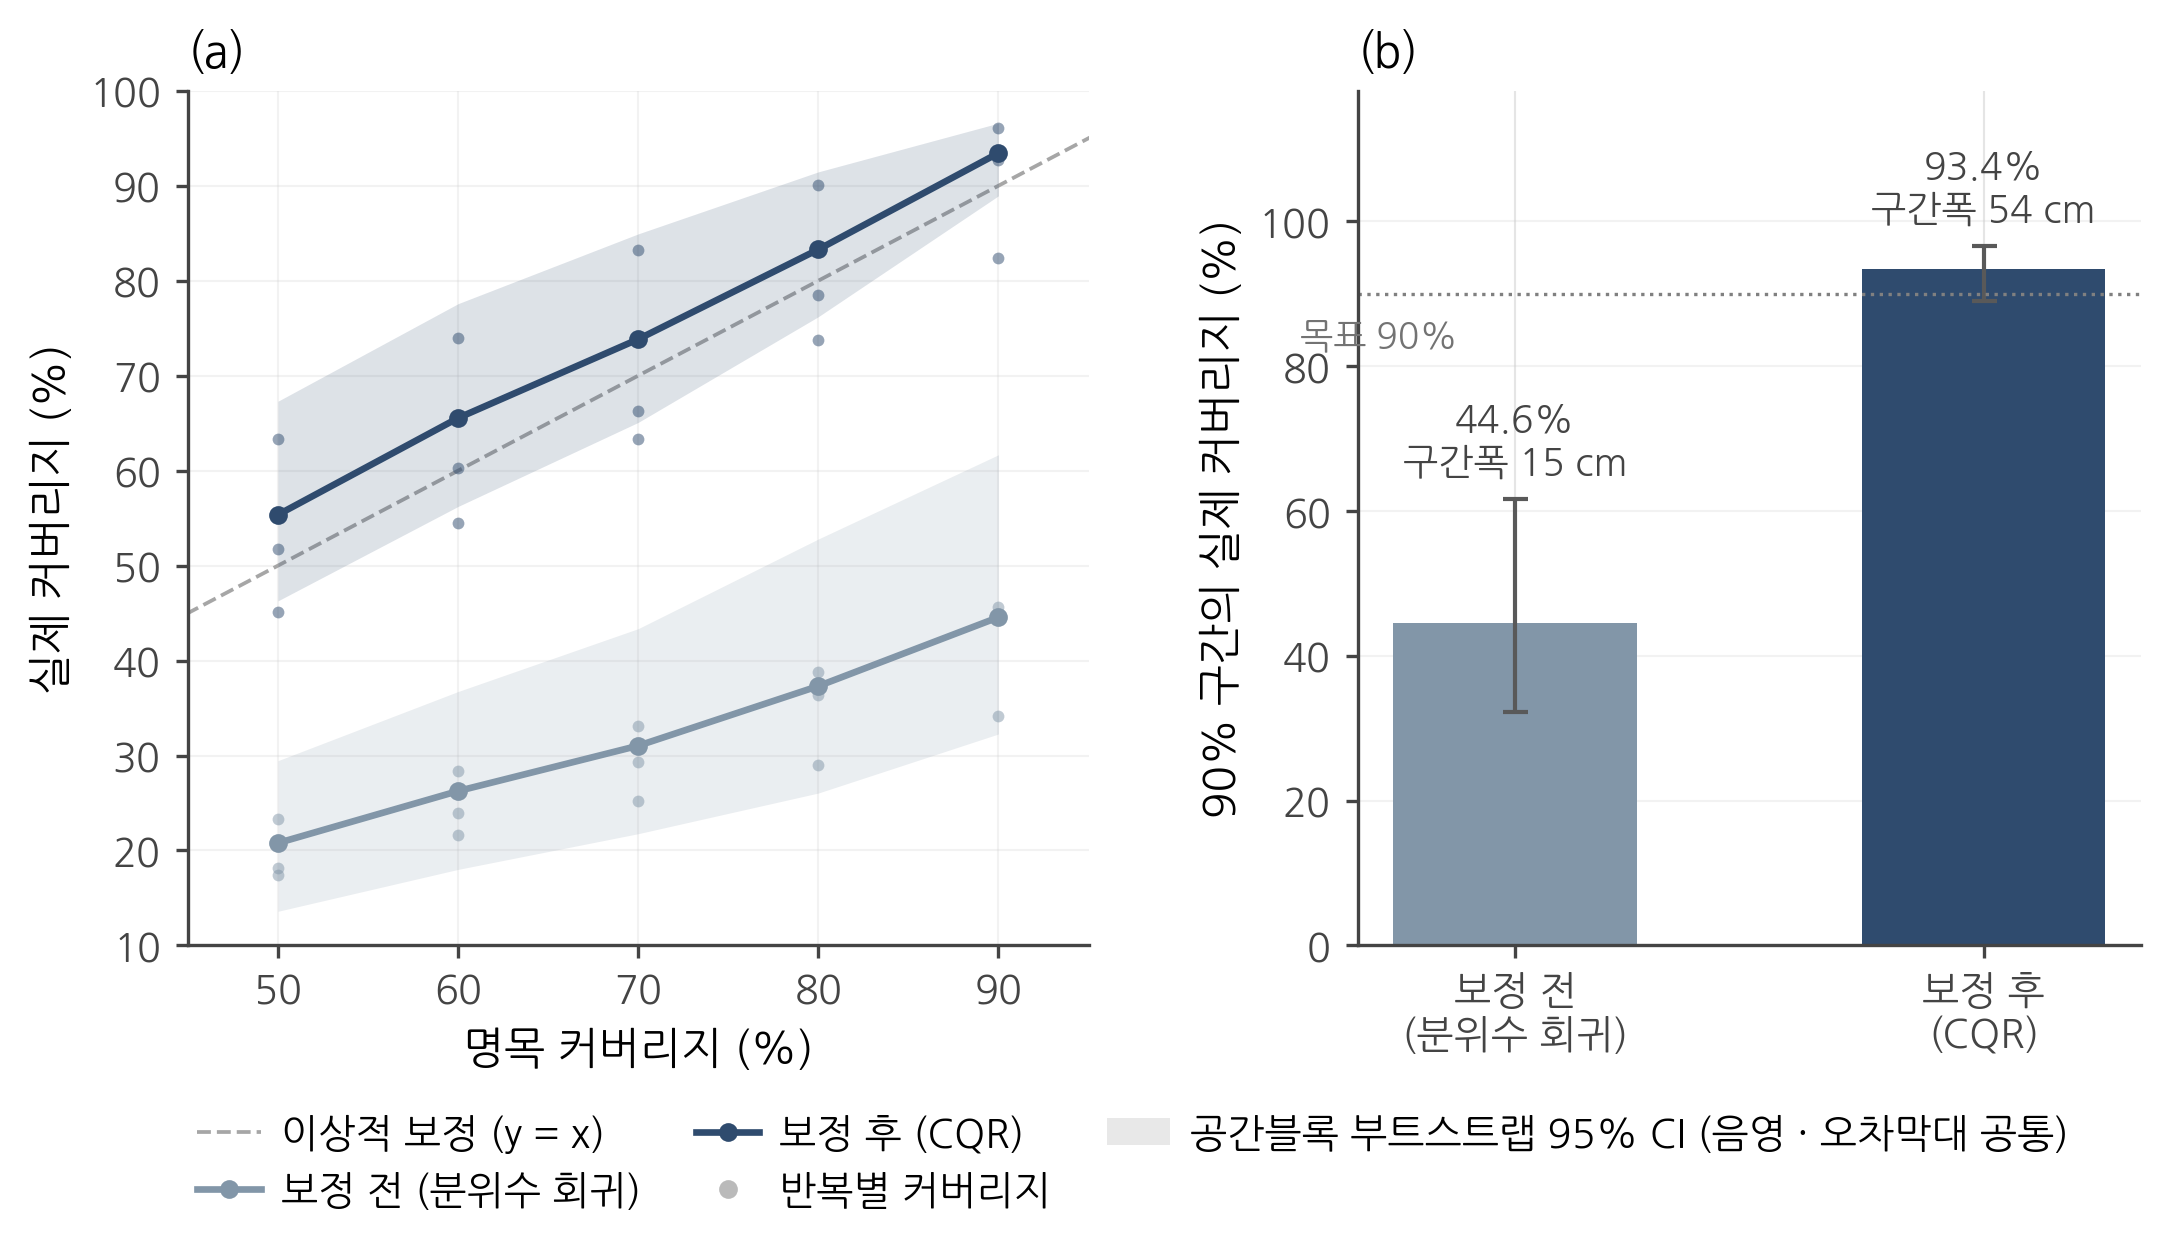
\includegraphics[width=\linewidth]{../figures/s11_uq/s11_calibration_curve.png}
  \caption{예측구간 보정(분위 회귀 + 등순응 보정, 알래스카 공간블록 교차검증). 원 분위 회귀의 과신을 등순응 보정이 교정한다. (a)의 음영과 (b)의 오차막대는 모두 공간블록 부트스트랩 $95\%$ CI이다.}
  \label{fig:calib}
\end{subfigure}\hfill
\begin{subfigure}[t]{0.50\textwidth}
  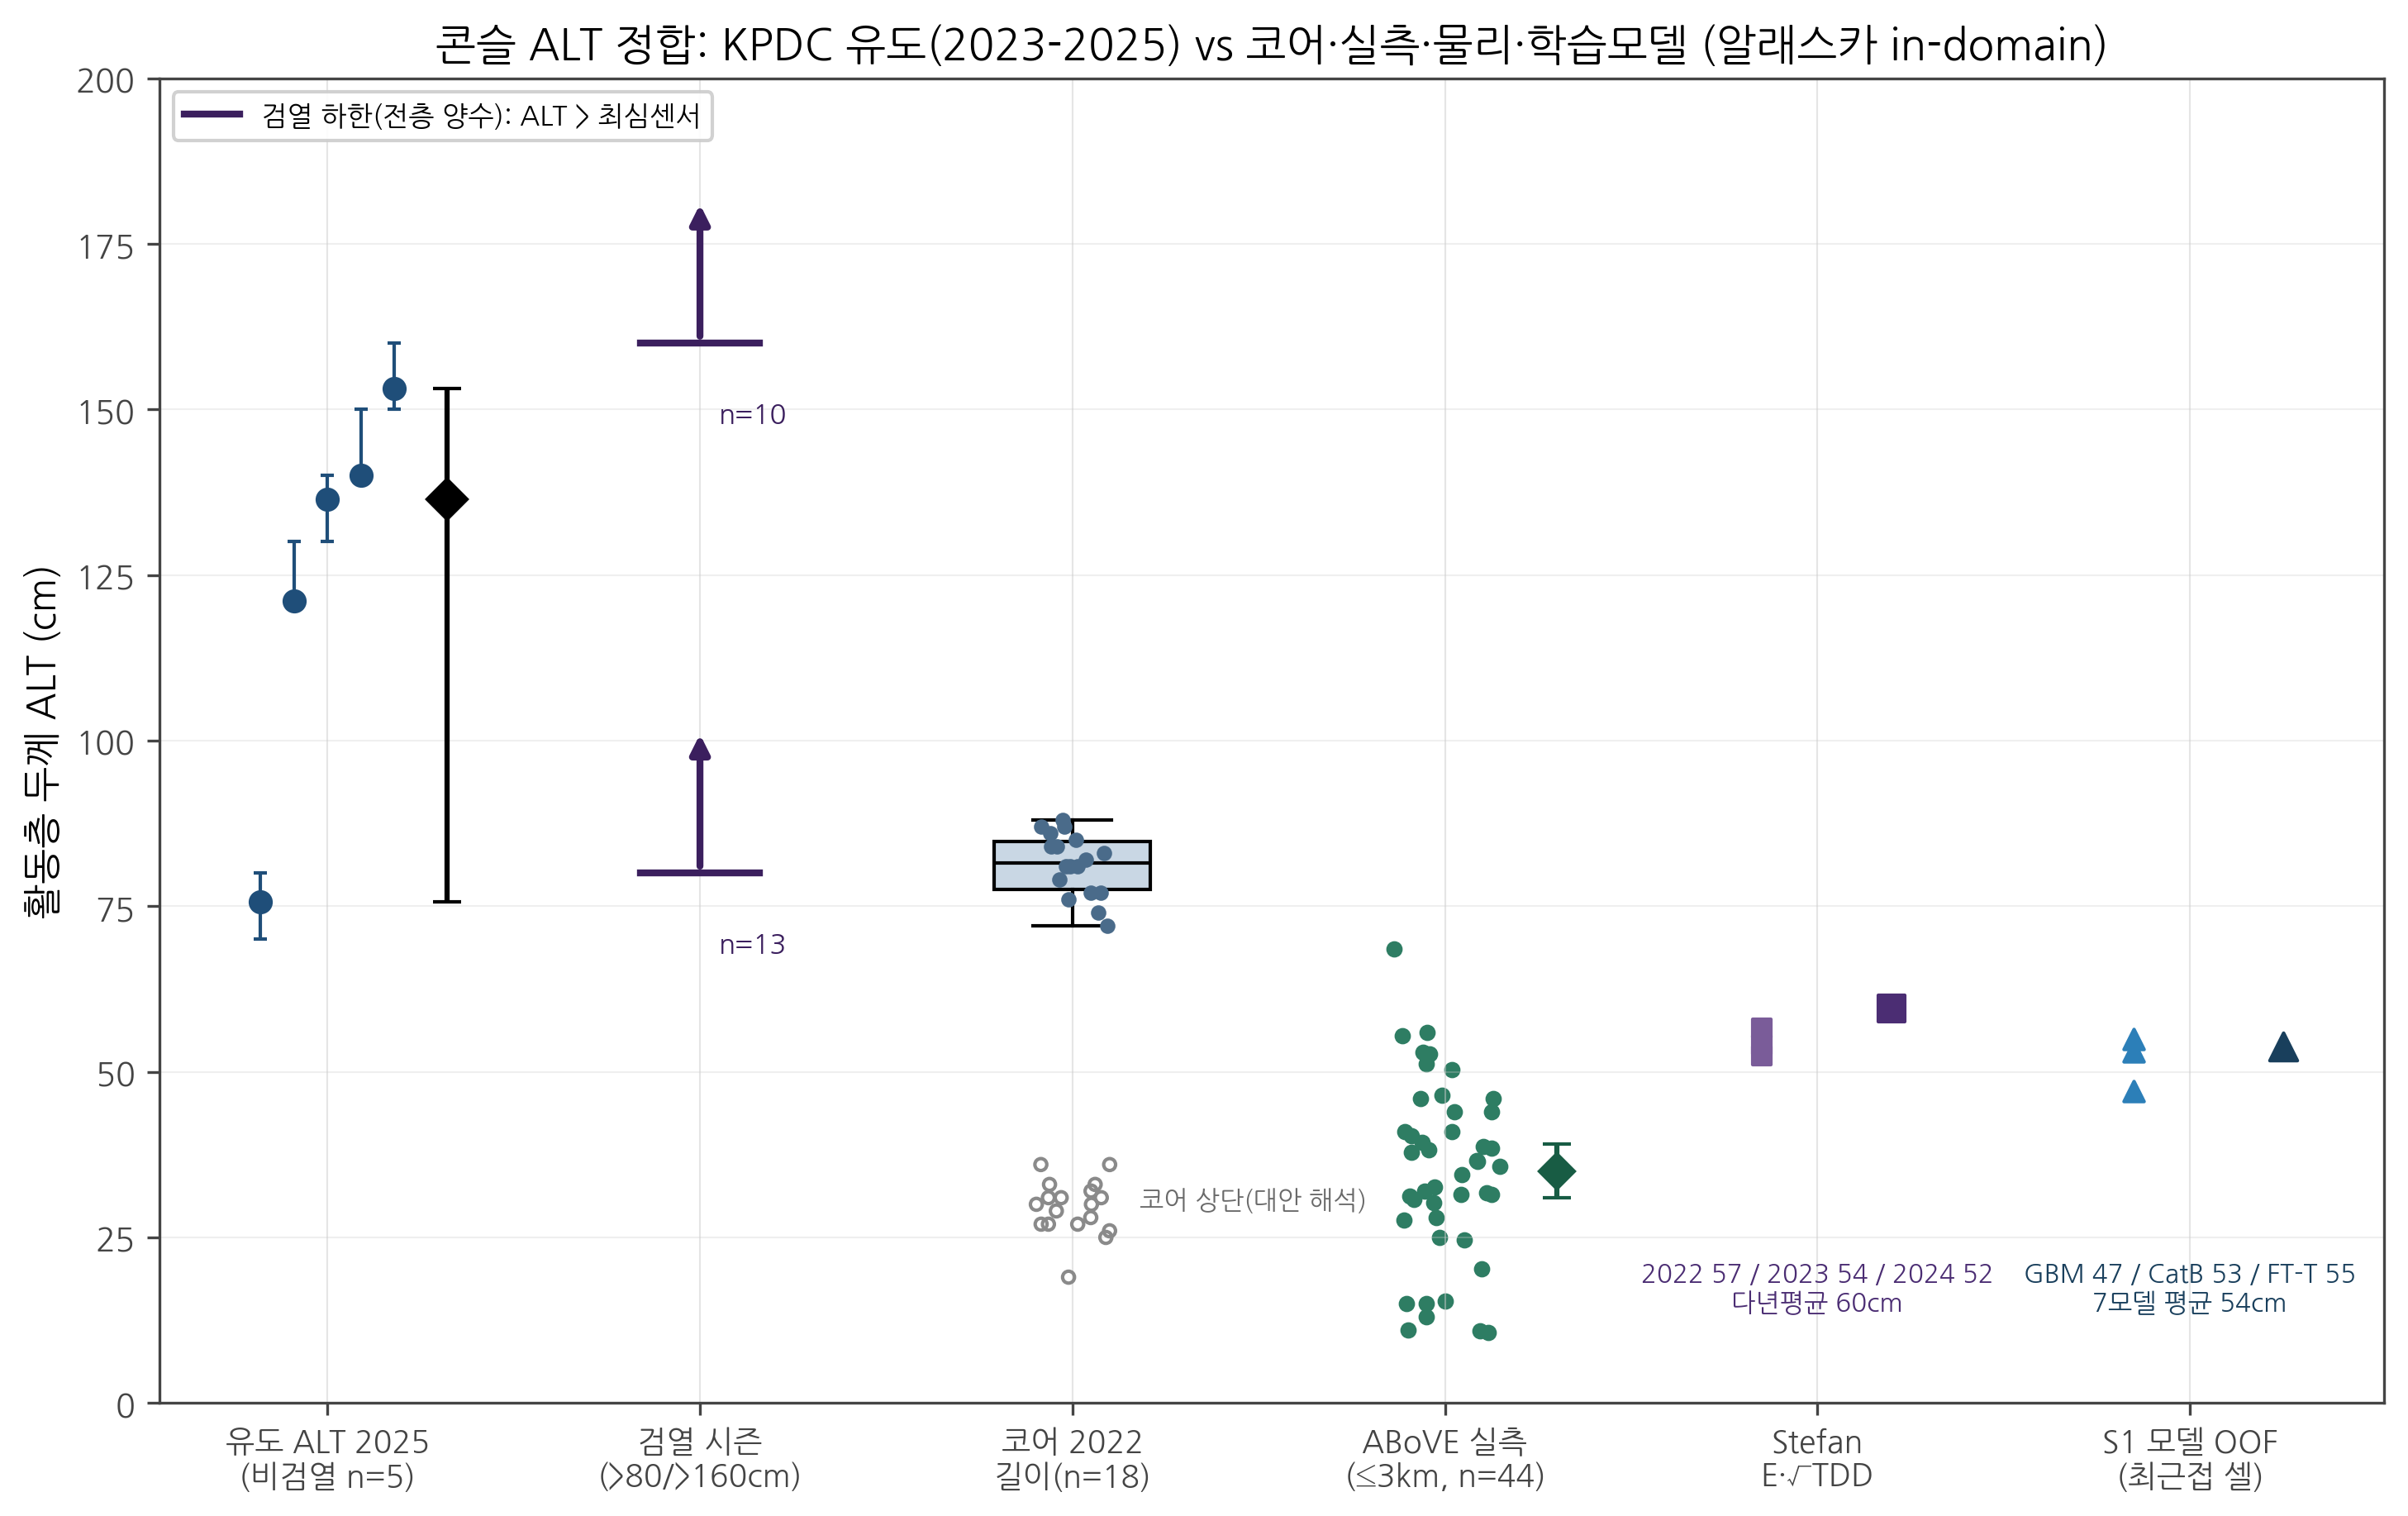
\includegraphics[width=\linewidth]{../figures/s7_kpdc/s7_alt_comparison.png}
  \caption{콘슬 ALT 유도 비교. 관측 방식에 따라 $35\text{--}136\,\mathrm{cm}$로 벌어진다. 개별 점의 세로선은 $0^\circ\mathrm{C}$ 교차를 감싸는 인접 센서 깊이 구간이고, 상자는 사분위수, 수염은 $1.5\times$IQR이다. $E\cdot\sqrt{\mathrm{TDD}}$는 Stefan 계수와 누적 융해도일 제곱근의 곱, 교차검증은 알래스카 공간블록 교차검증 예측이다.}
  \label{fig:kpdc}
\end{subfigure}
\caption{보정 불확실성과 KPDC 현장 검증.}
\label{fig:uq}
\end{figure*}

\begin{figure*}[!t]
\centering
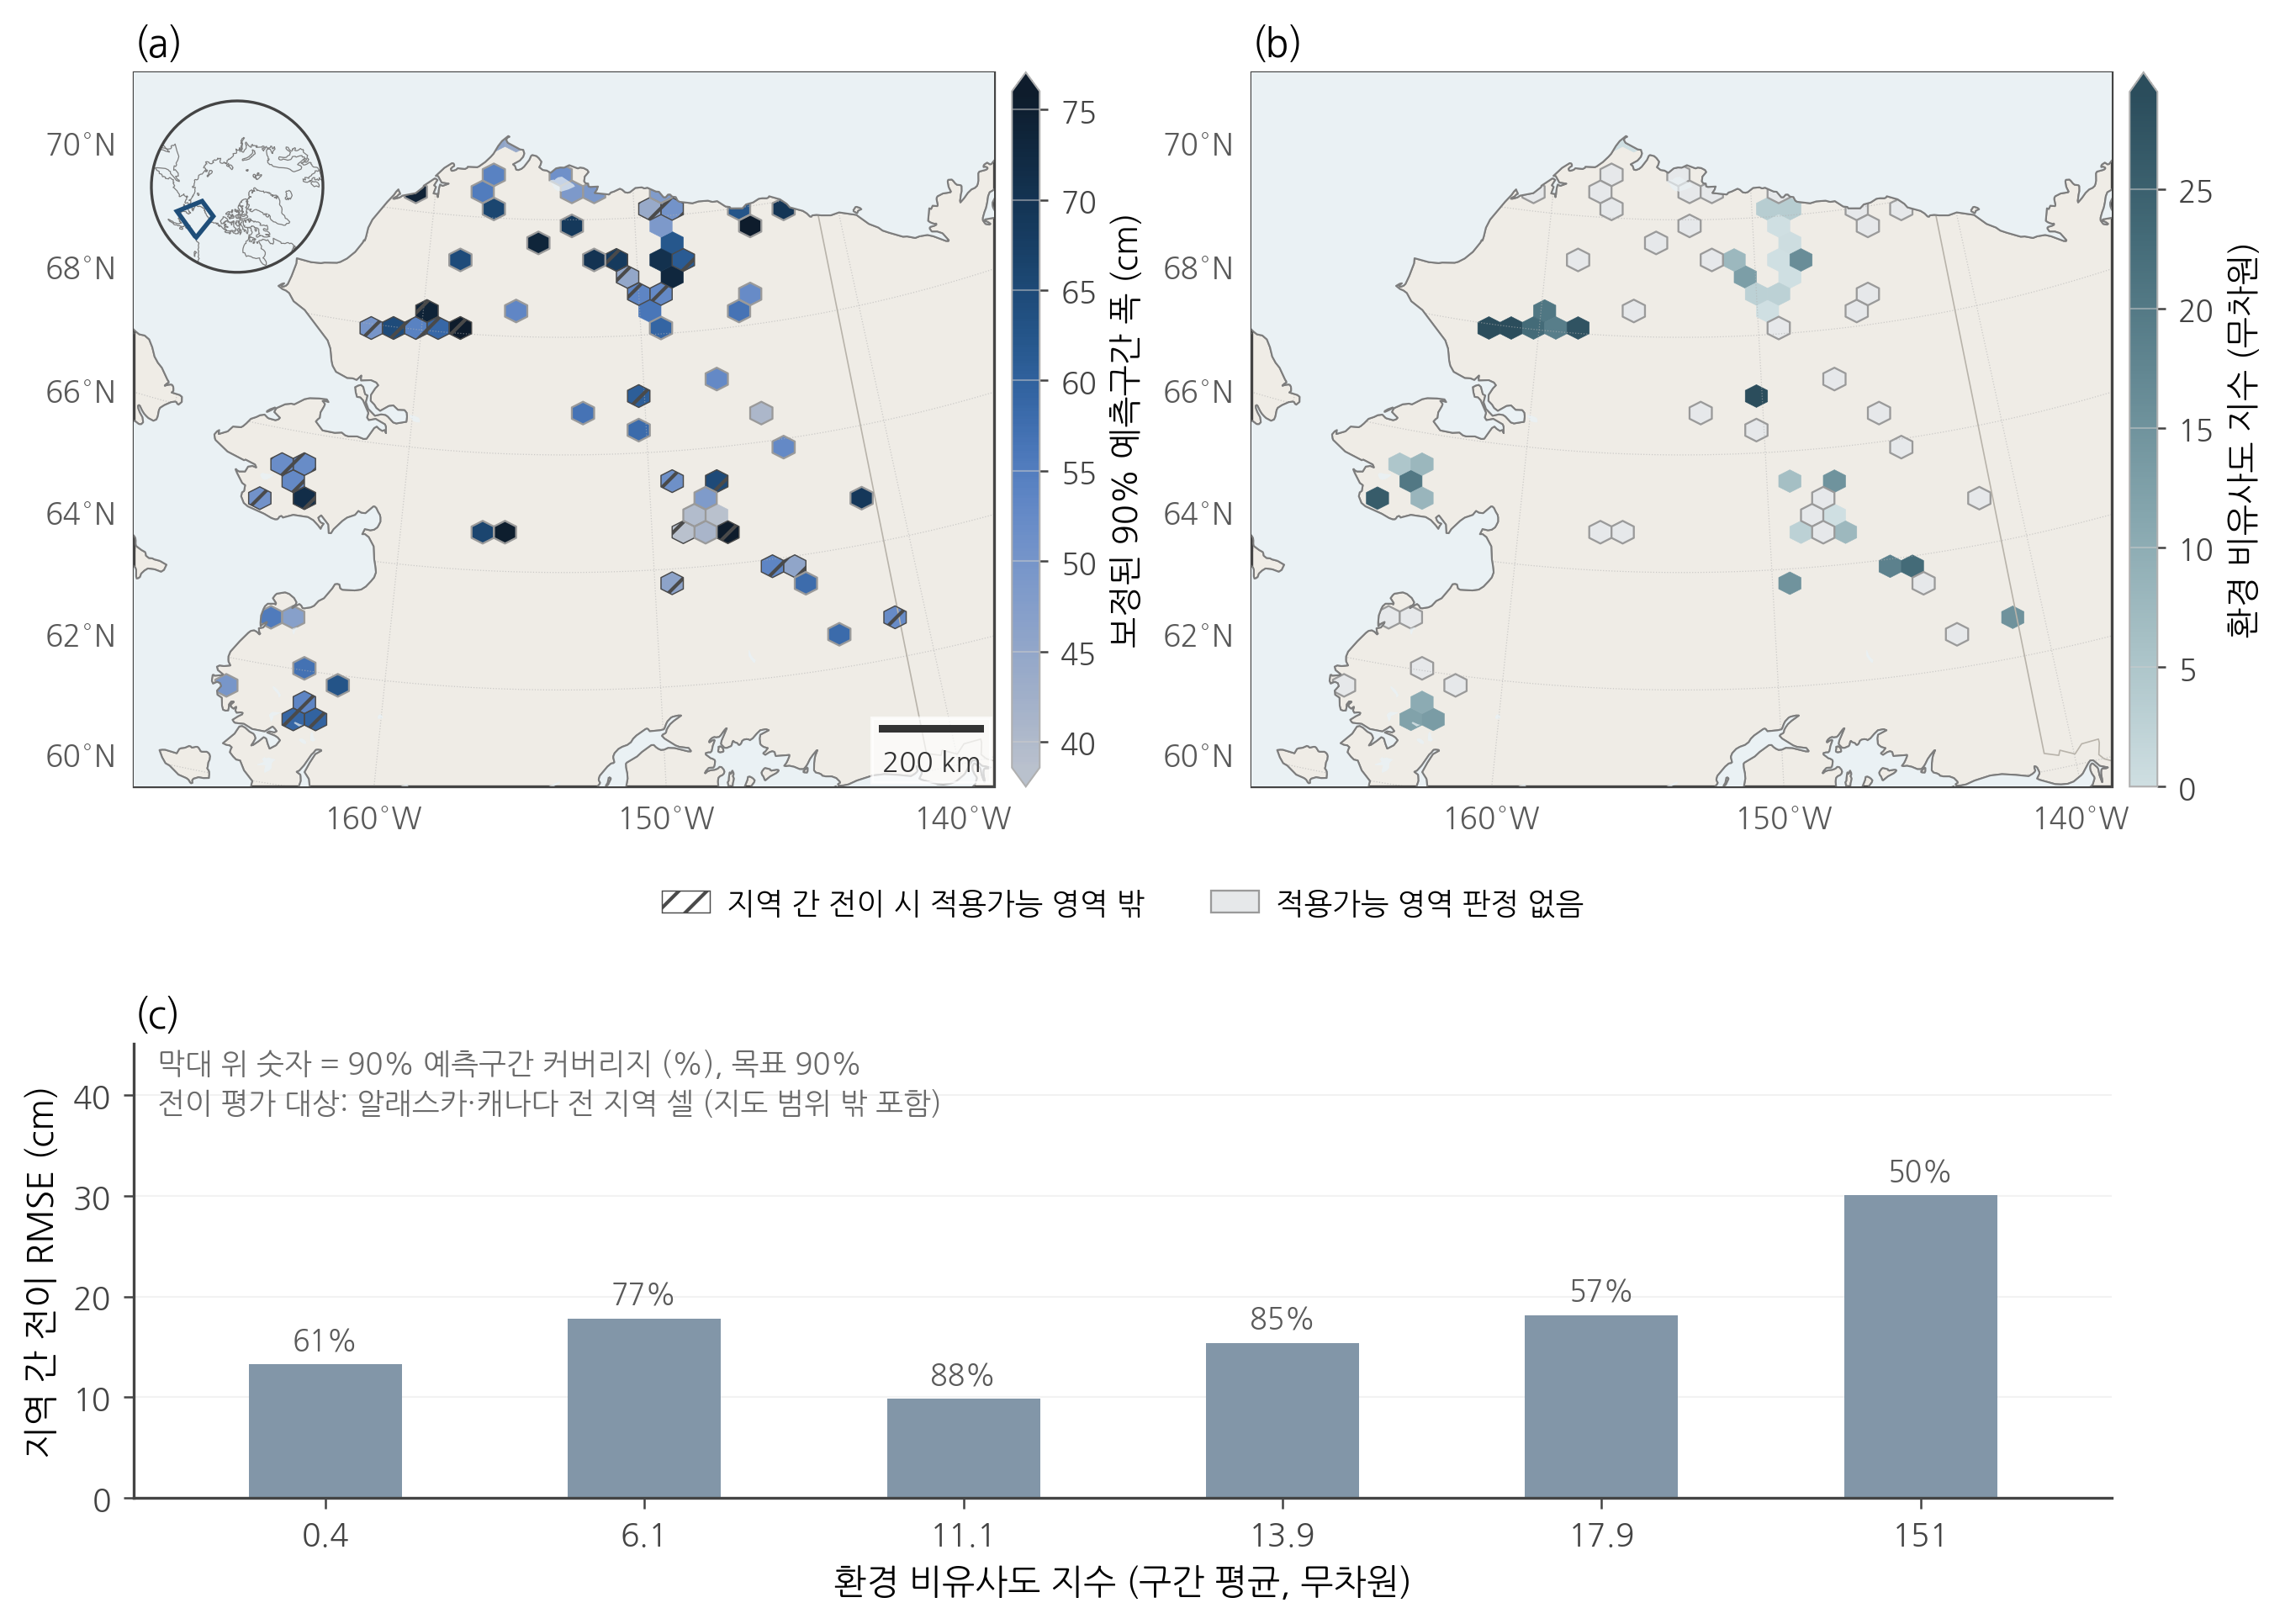
\includegraphics[width=0.86\textwidth]{../maps/alt_uncertainty_aoa_map.png}
\caption{예측의 신뢰 범위 지도(등순응 보정 분위 회귀, 입력 25종). (a) 보정된 $90\%$ 예측구간의 폭. 빗금은 다른 지역으로 전이할 때 적용가능 영역을 벗어나는 셀이다. (b) 학습 분포와의 환경 비유사도. (c) 비유사도 구간별 전이 오차와 실제 커버리지. 비유사도가 커질수록 오차가 늘고 커버리지가 목표에 미치지 못한다.}
\label{fig:uqmap}
\end{figure*}


% =====================================================================
\section{논의}
% =====================================================================

\subsection{강점과 차별성}
본 연구의 중심은 라벨 희소를 다출처 증강으로 완화하는 프레임워크이다. 실측·지중온도 유도·물리식 유도의 세 출처를 후보로 두고 검증을 거쳐 학습에 편입할 범위를 정하고, 물리식의 종류와 증강 비율, 학습 기법을 체계적으로 바꾸며 비교한 점이 기존 연구와 다르다. 특히 물리 유사라벨의 이득을 대조 실험으로 분리하여, 개선이 단순 라벨 추가가 아니라 물리 정보에서 온다는 것과 물리식의 정확도가 효과를 좌우한다는 것을 정량으로 보였다. 또한 전이 오차를 편향과 산포로 분해하여 개선의 여지가 어디에 있는지를 특정하고, 산출 원리가 다른 두 정보원을 결합해 편향을 상쇄하는 경로를 제시하였다. 순방향 시뮬레이션 위주였던 기존 연구[7,8]나 예측구간이 없는 광역 지도 제품[9,10,11]과 달리, 본 연구는 관측 라벨로 직접 평가되고 보정된 예측구간을 함께 제시한다. 물리 제약을 신경망 구조에 주입하는 방식을 기여로 삼은 최근 연구(지열 분야의 그래프 신경망[12], 청장고원 영구동토의 순환신경망[13])와 달리, 본 연구는 물리식을 라벨 생성기와 기준선으로 활용하여 라벨이 없는 지역까지 학습 신호를 확장한다.

\subsection{연구의 의의}
방법 측면에서 정확한 물리 유도 증강이 실측이 부족한 지역의 예측을 개선하는 실효 경로임을 확인하였고, 그 한계가 물리식이 담은 정보량에 있음을 밝혀 산출 방식이 다른 관측을 결합하는 다음 경로를 제시하였다. 산출물 측면에서는 단일 시점의 2차원 ALT 지도에 머무르지 않고 동일한 자료 기반 위에서 연별 ALT 지도와 표층 3차원 지중온도장을 함께 산출하여, 활동층을 시간과 깊이를 포함한 상태로 기술하였다. 신뢰 측면에서는 보정 예측구간과 적용가능 영역 표기로 사용자가 지도의 신뢰 범위를 판단할 근거를 제공하였다. KPDC 현장 자료는 이 모두의 전제인 공변량 기반이 현장과 정합함을 확인해 준다.

\subsection{한계와 극복 방안}
지점 관측은 미터 규모에서도 큰 공간변동을 보인다[6]. 이 변동과 콘슬 사이트의 관측 방식별 편차를 함께 보면 단일 지점 검증의 대표성 하한은 약 $10\text{--}12\,\mathrm{cm}$로 추정된다. 이는 검증을 면적평균 기준으로 전환하고 셀당 다점 평균을 도입하여 완화한다. 지역 간 전이에서는 물리식 단독이 가장 견고하였고, 잔차 결합과 유사라벨 증강은 이를 넘지 못하였다. 개선은 산출 방식이 다른 위성 제품을 결합하여 편향과 산포를 함께 줄이는 경로에서 나타났다. 대상 지역의 지중온도를 조밀하게 확보하면 유도 라벨의 품질이 높아져 증강 효과가 더 커질 것이다. 계절 융해의 시간 예측은 관측 기간을 늘리고, 일 단위 기온·적설 같은 기상 입력을 모델에 직접 제공하면 개선될 것으로 판단된다.

결합 효과의 유의성을 확정하지 못한 것도 표본의 제약에서 온다. 평가 단위인 공간블록이 지역당 $11\text{--}30$개에 그쳐 작은 개선을 가려낼 검정력이 부족하다. 이는 세 가지로 완화할 수 있다. 대상 지역을 시베리아 다른 유역이나 캐나다 군도로 넓히면 블록 수가 늘어 검정력이 직접 올라간다. 평가 단위를 지점이 아니라 InSAR 면적평균으로 바꾸면 같은 관측에서 더 많은 독립 표본을 얻을 수 있다. 결합 가중을 고정하지 않고 지역 특성에 따라 조절하면 개선폭 자체가 커져 같은 표본에서도 검출이 쉬워진다.

% =====================================================================
\section{결론}
% =====================================================================
본 연구는 실측 ALT가 희소하다는 영구동토 광역 예측의 근본 제약을, 라벨 자체를 늘리는 방향으로 해결하였다. 실측 ALT, 지중온도 프로파일에서 유도한 ALT, 물리경험식에서 산출한 ALT를 하나의 학습쌍 집합으로 결합하고, 그 위에서 기계학습·딥러닝으로 ALT를 예측하는 프레임워크를 구성하였다.

핵심 성과는 네 가지이다. 첫째, 정확한 물리경험식으로 생성한 유사라벨을 실측이 부족한 지역에 증강하면 예측 오차가 뚜렷이 감소하며, 그 이득이 학습쌍의 단순 증가가 아니라 물리 정보 자체에서 비롯됨을 대조 실험으로 분리하여 입증하였다. 동시에 부정확한 물리식을 증강하면 오히려 성능이 저하되므로, 증강의 성패는 물리식의 정확도에 달려 있음을 정량화하였다. 이는 물리 기반 증강을 적용하려는 후속 연구에 직접적인 설계 지침이 된다. 둘째, 물리경험식에 잔차 모델을 결합하여 알래스카 지역 내에서 $13.33\,\mathrm{cm}$의 오차를 달성하였다. 다만 이 우위는 학습 지역 안에서만 성립하며, 관측이 없는 지역으로 옮기면 잔차 항이 오히려 오차를 키운다. 지역 내 정확도와 전이 견고성은 잔차 가중을 사이에 두고 상반된다. 셋째, 전이 오차를 편향과 산포로 분해하여 개선 여지를 특정하고, 산출 방식이 다른 위성 관측 제품을 물리식과 결합하는 경로를 제시하였다. 오차 감소는 네 개의 지역·조건 조합에서 방향이 일관되었으나, 표본 블록 수의 제약으로 유의성 확정에는 이르지 못하였다. 넷째, 동일한 자료 기반 위에서 연별 ALT 지도와 표층 3차원 지중온도장을 함께 산출하여, 활동층을 단일 시점의 2차원 값이 아니라 시간과 깊이를 포함한 상태로 기술하였다.

아울러 보정된 예측구간과 적용가능 영역 표기로 각 지점의 신뢰 범위를 명시하였고, KPDC 현장 관측으로 기후 공변량 기반의 타당성을 확인하였다. 본 프레임워크는 실측이 희소한 다른 극지 변수에도 적용할 수 있으며, 대상 지역의 지중온도 관측을 조밀하게 확보할수록 유도 라벨의 품질이 높아져 증강 효과가 더욱 커질 것으로 기대된다.

% =====================================================================
\section*{참고문헌}
% =====================================================================
{\footnotesize
\begin{enumerate}[leftmargin=1.5em,itemsep=0pt,topsep=0pt,parsep=0pt,label={[\arabic*]}]
\item Schuur, E. A. G. et al. (2015). Climate change and the permafrost carbon feedback. \textit{Nature} 520, 171--179.
\item Hugelius, G. et al. (2014). Estimated stocks of circumpolar permafrost carbon with quantified uncertainty ranges and identified data gaps. \textit{Biogeosciences} 11, 6573--6593.
\item Hjort, J. et al. (2018). Degrading permafrost puts Arctic infrastructure at risk by mid-century. \textit{Nat. Commun.} 9, 5147.
\item Rantanen, M. et al. (2022). The Arctic has warmed nearly four times faster than the globe since 1979. \textit{Commun. Earth Environ.} 3, 168.
\item Biskaborn, B. K. et al. (2019). Permafrost is warming at a global scale. \textit{Nat. Commun.} 10, 264.
\item Nelson, F. E. et al. (1998). Active-layer thickness in north central Alaska: systematic sampling, scale, and spatial autocorrelation. \textit{J. Geophys. Res.} 103(D22), 28963--28973.
\item Jafarov, E. E., Marchenko, S. S., Romanovsky, V. E. (2012). Numerical modeling of permafrost dynamics in Alaska using a high spatial resolution dataset. \textit{The Cryosphere} 6, 613--624.
\item Riseborough, D. et al. (2008). Recent advances in permafrost modelling. \textit{Permafr. Periglac. Process.} 19, 137--156.
\item Obu, J. et al. (2019). Northern Hemisphere permafrost map based on TTOP modelling for 2000--2016 at 1\,km$^2$ scale. \textit{Earth-Sci. Rev.} 193, 299--316.
\item Ran, Y. et al. (2022). New high-resolution estimates of the permafrost thermal state and hydrothermal conditions over the Northern Hemisphere. \textit{Earth Syst. Sci. Data} 14, 865--884.
\item Obu, J. et al. (2019). ESA Permafrost CCI: Active Layer Thickness for the Northern Hemisphere, v3.0. CEDA. doi:10.5285/1ee56c42cf6c4ef698693e00a63795f4.
\item Aljubran, M. J., Horne, R. N. (2024). Thermal Earth model for the conterminous United States using an interpolative physics-informed graph neural network. \textit{Geotherm. Energy} 12, 25.
\item Liu, Y. et al. (2023). Multisite evaluation of physics-informed deep learning for permafrost prediction in the Qinghai--Tibet Plateau. \textit{Cold Reg. Sci. Technol.} 216, 104009.
\item Stefan, J. (1891). \"Uber die Theorie der Eisbildung. \textit{Ann. Phys.} 278, 269--286.
\item Kudryavtsev, V. A. et al. (1974). \textit{Fundamentals of Frost Forecasting in Geological Engineering Investigations}. Moscow Univ. Press (CRREL Draft Transl.\ 606, 1977).
\item Mu\~noz-Sabater, J. et al. (2021). ERA5-Land: a state-of-the-art global reanalysis dataset for land applications. \textit{Earth Syst. Sci. Data} 13, 4349--4383.
\item Meyer, H., Pebesma, E. (2021). Predicting into unknown space? Estimating the area of applicability of spatial prediction models. \textit{Methods Ecol. Evol.} 12, 1620--1633.
\item Romano, Y., Patterson, E., Cand\`es, E. J. (2019). Conformalized quantile regression. \textit{NeurIPS} 32, 3538--3548.
\item Prokhorenkova, L. et al. (2018). CatBoost: unbiased boosting with categorical features. \textit{NeurIPS} 31, 6638--6648.
\item Gorishniy, Y. et al. (2021). Revisiting deep learning models for tabular data. \textit{NeurIPS} 34.
\item Gorishniy, Y., Kotelnikov, A., Babenko, A. (2025). TabM: advancing tabular deep learning with parameter-efficient ensembling. \textit{ICLR}.
\item Brown, J., Hinkel, K. M., Nelson, F. E. (2000). The Circumpolar Active Layer Monitoring (CALM) program: research designs and initial results. \textit{Polar Geogr.} 24, 165--258.
\end{enumerate}
}


\vspace{1pt}
{\scriptsize\noindent\textbf{재현 정보.}\; 전 실험의 산출 자료와 교차검증 설정은 저장소의 결과 파일로 제공한다. 대회 요건에 따라 KPDC 콘슬 자료를 주된 현장 검증 축으로 사용하였다. 사전학습 모델과 생성형 인공지능 사용 내역, 각 자료원의 라이선스·기간·해상도는 제출 시 별첨 표로 명시한다.}

\end{document}
